% This template was initially provided by Dulip Withanage.
% Modifications for the database systems research group
% were made by Conny Junghans,  Jannik Strötgen and Michael Gertz

% Further modification based on Scientific Computing Master Thesis Template

\documentclass [
     12pt,         % font size
     a4paper,      % paper format
     BCOR10mm,     % binding correction
     DIV14,        % stripe size for margin calculation
     liststotoc,   % table listing in toc
     bibtotoc,     % bibliography in toc
     idxtotoc,     % index in toc
     parskip       % paragraph skip instad of paragraph indent
     ]{scrreprt}

%%%%%%%%%%%%%%%%%%%%%%%%%%%%%%%%%%%%%%%%%%%%%%%%%%%%%%%%%%%%

% PACKAGES:

% Use German/English :
%\usepackage[ngerman]{babel}
\usepackage[english]{babel}

% Input and font encoding
\usepackage[latin1]{inputenc}
\usepackage[T1]{fontenc}

% Index-generation
\usepackage{makeidx}
% Einbinden von URLs:
\usepackage{url}
% Special \LaTex symbols (e.g. \BibTeX):
\usepackage{doc}
% Include Graphic-files:
\usepackage{graphicx}
\usepackage{caption}
\usepackage{subcaption}
\usepackage{array}



% Include doc++ generated tex-files:
%\usepackage{docxx}
% Include PDF links
%\usepackage[pdftex, bookmarks=true]{hyperref}

% Fuer anderthalbzeiligen Textsatz
\usepackage{setspace}

% hyperrefs in the documents
\usepackage[bookmarks=true,colorlinks,pdfpagelabels,pdfstartview = FitH,bookmarksopen = true,bookmarksnumbered = true,linkcolor = black,plainpages = false,hypertexnames = false,citecolor = black,urlcolor=black]{hyperref} 
%\usepackage{hyperref}

% maths equations
\usepackage{amsmath}
\usepackage{amssymb}


\usepackage{listings}% http://ctan.org/pkg/listings

% paragraph indentation and spacing
\setlength{\parindent}{0em} 
\setlength{\parskip}{1.5em}

%%%%%%%%%%%%%%%%%%%%%%%%%%%%%%%%%%%%%%%%%%%%%%%%%%%%%%%%%%%%

% OTHER SETTINGS:

% Pagestyle:
\pagestyle{headings}

% Choose language
\newcommand{\setlang}[1]{\selectlanguage{#1}\nonfrenchspacing}


\begin{document}

% Title 
% TITLE:
\pagenumbering{roman} 
\begin{titlepage}


\vspace*{1cm}
\begin{center}
\vspace*{3cm}
\textbf{ 
\Large Heidelberg University\\
\smallskip
\Large  Faculty of Mathematics and Computer Science\\
\smallskip
\Large  Institute of Computer Science\\
\smallskip
\Large Database Systems Research Group\\
\smallskip
}

\vspace{3cm}

\textbf{\large Master Thesis in Scientific Computing}  

\vspace{0.5\baselineskip}
{\huge
\textbf{Building a Map of Explicit Causal Factors from Financial Documents}
}

%%%% TO BE REMOVED BEFORE FINAL VERSION
\vspace{0cm}
----------------------------------------------------------------------------------------------
{\huge \textbf{[DRAFT as of \today] } }
----------------------------------------------------------------------------------------------
%%%% TO BE REMOVED BEFORE FINAL VERSION



\end{center}

\vfill 

{\large
\begin{tabular}[l]{ll}
Name: & Claire Zhao Sun\\
Matriculation Number: & 3630998\\
Supervisor: & Prof. Dr. Michael Gertz\\
Submission Date: & 2022.05.30
\end{tabular}
}

\end{titlepage}




%% Titleintro
%\thispagestyle{empty}
%\begin{center}
%  \renewcommand{\baselinestretch}{2.00}
% \Large\sffamily
%  Department of Mathematics and Computer Science\\
%  \large University of Heidelberg
%  \par\vfill\normalfont
%  Master thesis\\
%  in Scientific Computing\\
%  submitted by\\
%  (name and surname)\\
%  born in (place of birth)\\
%  (year of submission)
%\end{center}
%\newpage

%% Titlepage
%\thispagestyle{empty}
%\begin{center}
%  \renewcommand{\baselinestretch}{2.00}
%  \Large\bfseries\sffamily
%    (Title)\\
%    (of)\\
%    (Master thesis)
%  \par
%  \vfill
%  \large\normalfont
%  This master thesis has been carried out by (Name Surname)\\
%  at the\\
%  (institute)\\
%  under the supervision of\\
%  (Frau/Herrn Prof./Priv.-Doz. Name Surname)
  %% additionally insert second supervisor here if applicable
%\end{center}\par
%\vspace{5\baselineskip}

% reset baselinestretch
%\renewcommand{\baselinestretch}{1.00}\normalsize

% Declaration
\setlength{\parindent}{0em}

Erkl\"{a}rung:\par
\vspace{2\baselineskip}
Ich versichere, dass ich diese Master-Arbeit selbstst\"{a}ndig verfasst und nur die angegebenen
Quellen und Hilfsmittel verwendet habe und die Grunds\"{a}tze und Empfehlungen "Verantwortung in der Wissenschaft" der Universit\"{a}t Heidelberg beachtet wurden. 

\vspace*{50pt}
\noindent

\underline{\phantom{mmmmmmmmmmmmmmmmmmmm}}

\medskip
\noindent
 
Abgabedatum: 2022.05.30





\vspace{10\baselineskip}

Declaration:\par
\vspace{2\baselineskip}
I hereby confirm that I wrote this Master Thesis independently and only used the specified sources, based on the principles and recommendations of "Responsibility in Science'' of Heidelberg University.
\par

\vspace*{50pt}
\noindent

\underline{\phantom{mmmmmmmmmmmmmmmmmmmm}}

\medskip
\noindent 
Submission Date: 2022.05.30



\newpage


% Add a brief summary of your topic and contributions (Zusammenfassung) in German *and* in English:
\chapter*{Zusammenfassung}

% This file contains the German version of your abstract, with about 300-500 words

Die Zusammenfassung muss auf Deutsch \textbf{und} auf Englisch geschrieben
werden. Die Zusammenfassung sollte zwischen einer halben und einer
ganzen Seite lang sein. Sie soll den Kontext der Arbeit, die
Problemstellung, die Zielsetzung und die entwickelten Methoden sowie
Erkenntnisse bzw.~Ergebnisse �bersichtlich und verst�ndlich
beschreiben.
\newpage

\chapter*{Abstract}

% This file contains an abstract of your thesis, with approximaltely 300-500 words

The abstract has to be given in German \textbf{and} English. It should
be between half a page and one page in length. It should cover in a
readable and comprehensive style the context of the thesis, the
problem setting, the objectives, and the methods developed in this
thesis as well as key insights and results.

\newpage


% MAIN PART:
% Table of contents (Inhaltsverzeichnis)
\tableofcontents
\cleardoublepage
\pagenumbering{arabic} 

% List of figures (Abbildungsverzeichnis):
%\listoffigures
% List of tables (Tabellenverzeichnis):
%\listoftables


%%%%%%%%%%%%%%%%%%%%%%%%%%%%%%%%%%%%%%%%%%%%%%%%%%%%%%%%%%%%%%%
% Here, the actual content of your thesis begins
% You can either put all the text here or use individual files to store the chapters of your thesis.
% Below are templates for both alternatives.

\chapter{Introduction}\label{introduction}

%\chapter{Introduction}\label{introduction}

%[What is text mining. Some example applications in finance]
Text mining, also known as text analytics, is the process of applying Natural Language Processing (NLP) and Machine Learning (ML) techniques to automatically extract structured information from unstructured texts. The extracted information can be analysed to reveal hidden patterns and new insights, thus leading to knowledge discovery. While widely applicable and relevant to practically all business sectors, text mining has attracted, in particular, a lot of attention and excitement from the finance industry \cite{MLinFinance2021, TextMiningFinancialSector2019}. Major financial institutions and service providers are eager to embrace the advent of automatic text mining tools to deal with the huge amount of text-based documents, in anticipation of improved scalability, efficiency and information advantage \cite{MLinUKFin2019, FadorFuture2018}. Indeed, many successful applications, such as text classification, sentiment analysis, fraud detection, machine translation, speech recognition, etc., have been deployed in various subsectors of the finance industry \cite{Tueregun2019, Gupta2020, Ravula2020}.

%[Zoom in on investment research, highlight natural fit with text mining; lack of practical tools]
One particular subsector in finance that could greatly benefit from text mining is investment research. Underpinning the investment decision-making process, investment research is typically based on a thorough exploration of all information available on a given company or sector, in order to identify the underlying trends that may ultimately lead to profitable investment opportunities. This process closely echoes the two subfields of text mining, i.e., information extraction and knowledge discovery. Despite this, in practice, most investment research is conducted manually by financial analysts, to the best of my knowledge.

%[Limitations of existing methods. Gaps in expectation from industry]
This is not surprising, given the limitations of what the currently available text mining tools are capable of compared to the research requirements of the investment community. Firstly, the most successful ML models adopted in practice are based on supervised learning \cite{TextMiningFinancialSector2019, FadorFuture2018, Tueregun2019, Gupta2020}. Whether for sentiment analysis, fraud detection or text classification, the underlying models are essentially classifiers trained on large sets of annotated data, where simple ground truth labels are assumed to be available. However, this is generally not the case for investment research, where problems are complex, answers are subjective, and the ground truth is often not readily discernible. Rather than classification, data exploration and pattern recognition are more relevant to investment research.  

Secondly, based on my own experience, in practice, even when tasks can be reduced to classification problems, the amount of data available is often insufficient to properly train deep learning models. Furthermore, due to the sensitivity of proprietary information and the cost of data annotation, it is likely impractical to adopt the supervised machine learning approach used in so many other fields. 

Thirdly, most of the existing text mining tools based on ML usually adopt a black-box approach which often lacks interpretability. From my observations, the prevailing standard practice in investment research is to apply explicit causal inference through logical reasoning based on discrete and limited data points to explain market phenomena. Investment analysts simply cannot rely on ML models she/he does not understand or cannot explain. 


\section{Motivation}

% [direction of this thesis – solving a practical problem]
Recognizing the limited deployment of text mining tools in investment research, this thesis aims to build an automatic and intelligent system that can effectively help investors. Extracting causal factors from financial reports is one area that can be potentially aided by text mining. This particular focus stems from three real-life observations of how human analysts approach investment research. 

% [financial reports a great source of information –> our primary data source]
1. Financial reports are a primary source of information about publicly listed companies. A crucially important aspect of an analyst's day-to-day job is to gather financial data and business intelligence. These can be collected from a variety of sources, including, but not limited to, news media, industry conferences, company site visits, management interviews, etc. That said, a company's regulatory filings constitute an indispensable primary source of periodic information. These regulatory filings include financial reports such as 10-Q (quarterly reports) and 10-K (annual reports), in which it is required for management to present the companies' financial situation and explain their financial performance. Research analysts and investors alike usually scrutinize these reports in order to more deeply understand companies' business models and performance. Hence, this thesis chooses financial reports as its primary data source.

%[credit attribution, causal mining, common sense reasoning –> infuse heuristics, automated] the underlying causal factors driving their performance. 
2. Analysts intuitively perform causal inference, leveraging their prior knowledge and experience, when reading financial reports. When analysts try to figure out a company's business model or the sector trends that affect a company's performance, they look for the explicit credit attribution in the section of Management's Discussion and Analysis (MD\&A). They apply common sense reasoning to extract the causal financial performance factors (CFPFs) from this section and build mental models based on logical chains of events. CFPFs enable a better understanding of how the business operates under different scenarios which is useful for forecasting future performance. This process is closely related to causality mining in text analytics \cite{Ali21Survey,Yang21Survey}. Thus, this thesis endeavors to automate the extraction of CFPFs to facilitate this process.


%[long term trends, connecting the dots -> comprehensive, exploration at scale, accessible to all][data base at scale with accuracy] 
3. Experienced financial analysts accumulate sector knowledge through years of following certain companies in one particular sector; they have the ability to 'see' long-term trends and patterns by 'connecting the dots'. They do this through abstraction and recognizing patterns given only sparse data points. This, in turn, enables them to discover and identify unique investment opportunities. 

However, from the perspective of an investor or portfolio manager there are limitations with this approach. Each analyst tends to specialize in only one sector, so many are required to gain a comprehensive understanding of global equity markets. This can quickly become prohibitively expensive for all but the largest financial institutions. Furthermore, this specialization often makes it difficult to discern the larger picture of the economy, so broader market trends, such as inflation, are sometimes missed.  
Additionally, this knowledge and industry insight is stored in the analysts' minds and only conveyed through written reports or conference calls. Therefore, it is not readily accessible on demand to the investors who rely on it.  It would be useful to have a structured data model to store all of this knowledge at scale for programmatic exploration or integration with investment strategy simulations. 


%to infuse this prior expert knowledge in the system. Mimic the human behaviour and leverage expert's heuristics as much as possible while making the process as automated. Abstraction and high-level abstract thinking. Causality inference. Not just data driven. Graphs. We do not teach our children labels and data samples. We teach them rules. Analysts undergoing trainings before job to learn the basic concepts and causality in finance. Association learning. Preprocessing steps to help computer to process in a more structured way. Heuristics rules infused with prior knowledge and expert experience rather than merely labelled training data annotation//and organize them in a structured data model. Rule-based heuristics rather than complete reliance on supervised ML and Data driven models. Expert system with human infused knowledge is a better hybrid approach.


%[caveats: financial reports only part of the information; investment is multi-faceted; not to replace human completely; help do the heavy lifting, nowhere close to GAI, human-machine interaction] 
Investment research is a complex, multi-faceted process which requires a comprehensive skill-set, including financial and accounting literacy, critical thinking, problem solving, data gathering, analytical skills, etc. Human analysts play a vital role in this laborious process. Due to the fact that text mining tools based on ML models available today are nowhere close to achieving general intelligence, it is infeasible to design a system which could replace human analysts. Rather, it would be more effective to compliment human analysts' existing skills by providing partial automation, letting computers do the heavy lifting of data processing, and empowering analysts to focus on data exploration and pattern discovery. 
The key motivation of this thesis is to inspire the creation of a tool that promotes human-machine interaction to assist investors, portfolio managers, and financial analysts through the provision of efficient information extraction required for the identification of investment opportunities.


\section{Objectives}

Recognizing the lack of text mining tools that help tackle practical problems faced daily in investment research, this thesis aims to build an end-to-end pipeline for causality mining from financial reports. The main contributions of this thesis are summarized as follows:

\begin{itemize}

\item We design a heterogeneous graph-based data model to represent companies, financial reports, and the relevant contents therein. This data model facilitates data exploration and knowledge discovery.  
\item We implement causality extraction based on linguistic patterns and heuristic rules to identify the business drivers and financial performance factors explicitly mentioned in the financial reports. This results in better explanability and interpretability. 
\item We enrich this data model with an abstraction layer using text clustering to make it easier to establish connections between causal factors and identify patterns in the underlying data model. By applying unsupervised clustering techniques, we effectively avoid issues associated with supervised learning (e.g., cost and data annotation)
\item [?modify?] We also demonstrate a proof-of-concept visualization for data exploration and discovery of previously unknown patterns. We showcase human-machine interaction and how we can leverage machine learning to complementary human.

\end{itemize}



\section{Outline}

This thesis is structured as follows. Chapter \ref{introduction} introduces the motivation for this thesis and outlines its main objectives. Chapter \ref{background} provides a comprehensive overview of fundamentals, such as various NLP techniques, causality extraction, clustering algorithms and related works. Chapter \ref{conceptualization} proposes a conceptual heterogeneous graph-based data model with customized node embeddings and similarity measures. Chapter \ref{implementation} introduces the data set and end-to-end pipeline to implement this model. Extensive experiments have also been performed on the model with results compared and discussed. Chapter \ref{conclusion} concludes this thesis with an outlook for future work. 




\newpage

%%%%%%%%%%%%%%%%%%%%%%%%%%%%%%%%%%%%%%%%%%%%%%%%%%%%%%%%%%%%

\chapter{Background and Related Work} \label{background}

%\chapter{Background and Related Work} \label{background}

This chapter covers the essential background and related work for subsequent chapters. Section \ref{sec:CE} begins with an introduction of causality extraction in the context of text mining. Three main approaches are described: 1. linguistic patterns and rule-based, 2. traditional ML based on manual feature selection, and 3. neural network-based deep learning models. Section \ref{sec:clustering} introduces basic concepts and techniques in NLP, such as word embeddings and compositional representations. Subsequently, text clustering algorithms based on these embeddings are discussed. Section \ref{sec:financial} provides an overview of related work with respect to text mining in financial reports, specifically, the Management Discussion and Analysis (MD\&A) section. Relevant SEC regulations are briefly introduced to provide a background understanding of the the formats and contents of these filings. Finally, Section \ref{sec:related} highlights a select few papers that are most relevant to this thesis.



\section{Causality Extraction} \label{sec:CE}

\subsection{What is Causality Extraction}

Causality Extraction (CE), also known as causality mining, is a subfield of Information Extraction (IE), which itself is a subfield of Text Mining \cite{Yang21Survey,Ali21Survey}. See Figure \ref{fig:CETaxomony} for an overview of the taxonomy of the field, highlighting the key topic of this thesis, i.e., Causality Extraction, with respect to other relevant subfields. 

\begin{figure}[h!]
\centering
  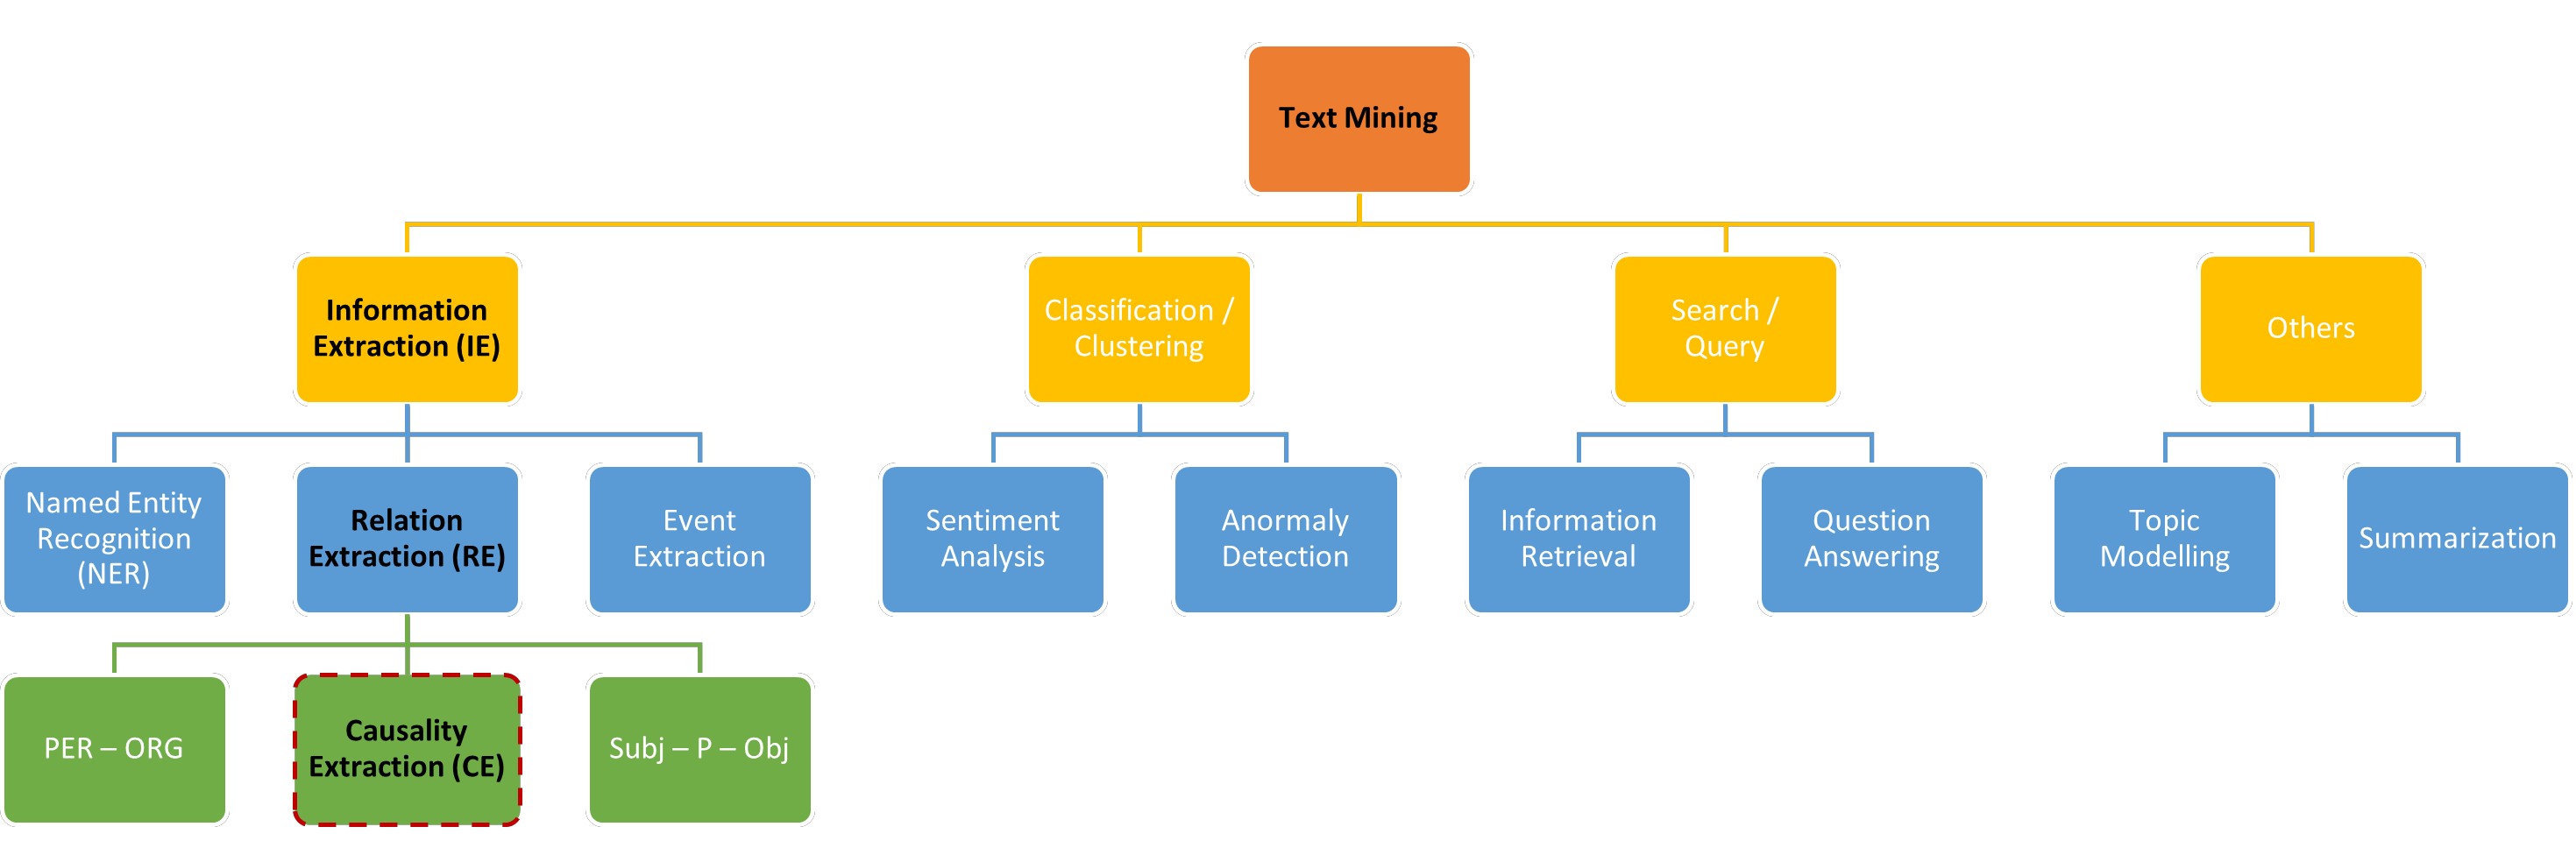
\includegraphics[scale=0.7]{figures/CETaxonomy.png}
  \caption{Causality Extraction's Position in the Taxonomy of Text Mining}
  \label{fig:CETaxomony}
\end{figure}


%[what is causality 0.5 page]
Causality is a type of relation between two events, states, phenomena or entities, in which one (referred as the \emph{cause}) triggers the other (referred as the \emph{effect}). Causal reasoning is the process of identifying causality. Understanding causality is a fundamental trait of human intelligence. We perform causal reasoning intuitively. However, it is often not a straightforward task to define what is \emph{cause} and what is \emph{effect}. The exact nature of \emph{cause} and \emph{effect} is indeed a metaphysical question that has sparked a long and deliberate philosophical debate which is still unresolved \cite{Ali21Survey}. 

Within the scope of this thesis, CE is defined in the context of NLP as the task of identifying the \emph{claimed} causal relation between a pair of events that are asserted in written texts \cite{causenet2020}, regardless of the nature and the validity of that relation in reality. In other words, there could be a disparity between the true causality in reality and the \emph{claimed} causality expressed in some given text. Due to the implicit nature of logic and the ambiguity of construction when expressing causal relations in natural language, it is a challenging task, for both humans and machines, to accurately identify exact causality \cite{DunietzThesis18}.


%[causality expression in language: explicit/implicit/ambiguous]
Causality can be expressed in a variety of ways in natural languages, using many different semantic representations and syntactic patterns. For example, it can be explicitly marked by certain words or phrases, such as \emph{because, due to, as a result of}, etc.  These words and phrases are often referred to as \emph{causal markers, causal links or causal connectives} \cite{KhooThesis95}. Causality can also be embedded in a sentence or a group of sentences in an implicit way. For instance, in the text \emph{"Thomas Cook's demise leaves its German operations hanging. More than 140,000 German holidaymakers have been impacted and tens of thousands of future travel bookings may not be honored."} \cite{FinCausal20}, the cause is in the first sentence and the effects are in the second sentence, however, there is an absence of explicit causal connectives linking the two. In addition, there can be cases where the causality is ambiguous and sometimes shared with other types of relations such as temporal, obligation, conditional dependence, etc. See examples in Table \ref{table:exampleSentences}  

\begin{table}[ht]
    \centering
	\begin{tabular}{{p{0.15\linewidth} p{0.6\linewidth} p{0.15\linewidth}}} 
		 \hline
		Connectives & Sentences & Causality \\
		 \hline\hline
		As & There was no debate \emph{as} the Senate passed the bill on to the House. & Causal  \\
		As & It has a fixed time, \emph{as} collectors well know. & Non-causal \\
		 \hline
		After & Bischoff in a round table discussion claimed he fired Austin \emph{after} he refused to do a taping in Atlanta. & Causal \\
		After & In stark contrast to his predecessor, five days \emph{after} his election he spoke of his determination to do what he could to bring peace. & Non-causal \\
		 \hline\hline
		\end{tabular}
	\caption{Examples of ambiguous causal connectives, sourced from \cite{Yang21Survey}}
	\label{table:exampleSentences}
\end{table}


Research in CE is not very well developed as compared with other subfields of NLP, such as machine translation, sentiment analysis, etc. Although it has gained traction in recent years, systematic studies and available datasets on causality are still rather limited \cite{Xu20Review}. Broadly speaking, CE is perceived as two subtasks by existing literature: 1) detection of whether a sentence contains a causal relation; 2) extraction of the relevant cause and effect chunks \cite{FinCausal20}. The first subtask is treated as a text classification problem and the second one a sequence tagging problem. 

\paragraph{Text Classification:} This category mainly concerns identifying whether a sentence contains a causal relation. It is typically framed as a binary classification aiming to distinguish causal sentences from non-causal ones. An additional subtask in this category is to determine the direction of causality. When a pair of chunks representing cause and effect is indicated in a sentence, the classifier also needs to discriminate the cause from the effect, i.e., this becomes a multi-class classification: cause-effect, effect-cause and non-causal. The majority of the existing studies belongs to this category \cite{FinCausal20, SemEval07Task4, SemEval10Task8}.

\paragraph{Sequence Tagging:} This category focuses on identifying the chunks in a sentence that represent cause, effect and causal connectives. This is usually treated as a sequence tagging task with a BIO-scheme (B: Beginning, I: Inside, O: Outside). The overall aim is to assign a tag to each word in the sentence. Figure \ref{fig:BIOtags} shows an example of such a tagging scheme \cite{Li21BiLSTMCRF}. Although this is also a classification task, the approach used is very different from Text Classification due to the presence of a sequence and the logical relationships between tags \cite{Ali21Survey, FinCausal20, Xu20Review}.

\begin{figure}[h!]
\centering
  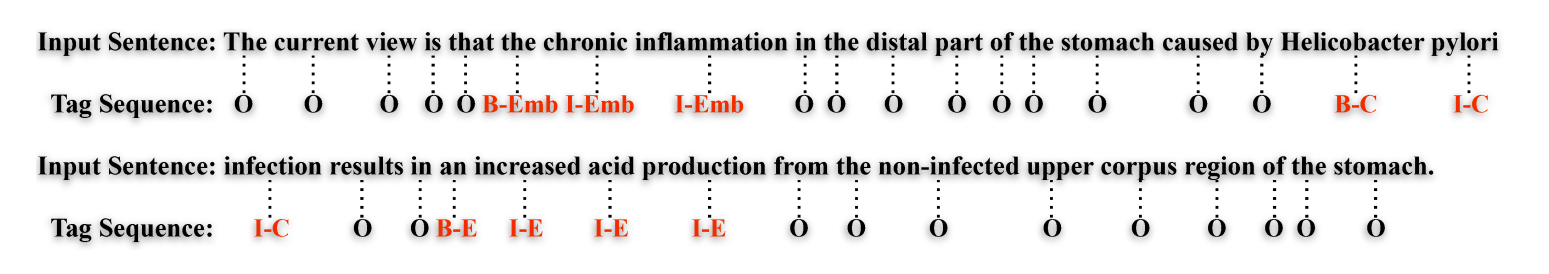
\includegraphics[scale=0.45]{figures/BIO.png}
  \caption{Illustration of Causality Sequence Tagging. Tag "O" represents the "Outside" or "None", which means that the corresponding word is irrelevant in any causality components. Tag "B-C" represents the "beginning of cause", tag "I-C" represents the "inside of cause", tag "B-E" represents the "beginning of effect", tag "I-E" represents the "inside of effect", tag "B-Emb" represents the "embedded causality begin", and tag "IEmb" represents the "embedded causality inside". Example sentence and tagging scheme taken from \cite{Li21BiLSTMCRF}.}
  \label{fig:BIOtags}
\end{figure}


\subsection{Techniques and Approaches}

% [Classification Approach: rule-based vs statistical ML vs NN/Deep Learning 2 pages]
In terms of techniques developed for CE, existing literature can be chronologically categorized into three stages: 1) linguistic pattern and rule-based approach; 2) traditional ML approach based on manual feature selection; 3) neural network-based deep learning approach. These approaches also echo the overall trends in NLP development, which has shifted from linguistic heuristics to statistical models, and now is moving increasingly towards the data-driven neural network architectures. Appendix \ref{appendix:CEpapers} shows a summary table of all the papers relevant to causality extraction reviewed for this thesis.



\subsubsection {\emph{1. Linguistic Patterns and Rule-based Approach}}

The focus of this particular approach is on cause and effect that is explicitly indicated in written English and only linguistic clues are used to identify causal relations. This method recognizes causal relations based on pre-defined lexico-semantic and syntactic patterns. These patterns can be expressed in terms of a sequence of words or syntactic categories that usually indicate the presence of a causal relation. 

The pioneering works developed by Khoo \cite{KhooThesis95,Khoo98,Khoo01} proposed three sets of such patterns: 1. patterns involving a causal link that links two phrases within a sentence (e.g., \emph{due to, because of}), 2. patterns involving a causal link that links two adjacent sentences (e.g., \emph{therefore, hence}), 3. patterns involving causal verbs and resultative constructions (e.g., \emph{cause, result in/from}). To identify causal relations in a document, a computer program locates all parts of the document that match with any of the linguistic patterns. "Slots" in these linguistic patterns indicate which part of the text is the cause and which the effect. For example, the pattern \emph{[effect] is the result of [cause]} indicates that the part of the sentence following the phrase \emph{is the result of} represents the \textbf{cause} and the part of the sentence preceding the phrase represents the \textbf{effect}.

Girju \cite{Girju02, Girju03} narrows the focus on the most frequently used causal verbs (e.g., \emph{cause, lead to, bring about}, etc.) and a specific lexico-syntactic pattern \emph{<noun phrase 1, verb, noun phrase 2>}. In contrast to Khoo's method where a whitelist of words have to be predefined manually, Girju's approach can automatically detect and acquire a list of verbs and verbal expressions, which is subsequently validated based on semantic constraints with the help of WordNet. In order to extract the corresponding cause and effect chunks, the model identifies noun phrases by matching the longest word sequence that is defined in WordNet as a concept. 

Similarly, Chan and Lam \cite{SEKE05} also include a WordNet-based component in their Semantic Expectation-based Knowledge Extraction (SEKE) framework for finding concepts synonymous to the extracted cause and effect phrases. This helps with disambiguation and also generates new causal patterns that were previously unseen. 

In order to minimize reliance on explicit pattern specification and achieve better generalization, Ittoo and Bouma \cite{IttooBouma11} develop a weakly supervised system that uses Wikipedia as a knowledge-base to automatically produce lexico-syntactic patterns. Using a bootstrapping method by taking some causal pairs (e.g., \emph{rain} and \emph{flood}) as seeds, their system first identifies causal links (e.g., \emph{leads to}) in Wikipedia that connect these seed pairs. It then selects the top $k$ most reliable causal link patterns to extract other candidate pairs (e.g., \emph{heat} and \emph{drought}) that are connected by the same causal link (i.e., \emph{leads to}). This recursive procedure of learning new patterns from seed and candidate pairs and vice-versa is repeated until some desired number of causal patterns have been harvested. Since their system does not rely on explicit causal markers or specified patterns, it can detect and extract implicit causal relations in texts. In addition, their lexico-syntactic patterns neutralize word order and morphological variations, in contrast to the conventional surface-strings from previous works.


\subsubsection {\emph{2. Traditional ML Approach based on Manual Feature Selection}}

One of the shortcomings of the linguistic pattern and rule-based approach is that it cannot distinguish causal and non-causal sentences that contain the same linguistic patterns or causal connectors. For example, both sentences (1) \emph{"It was the first time any of us had laughed since the morning began."} and (2) \emph{"He had to depend on himself, since he was miles away from others."} contain the connective \emph{"since"}, however, only (2) is causal whereas (1) is temporal. In order to disambiguate causal semantic relations from non-causal ones, a discriminative classifier is used. In this traditional ML approach, a classifier, such as Support Vector Machine (SVM), Maximum Entropy (ME), Naive Bayes (NB), and Logistic Regression (LG), is trained on the annotated dataset with hand-engineered features, such as word position, part-of-speech (POS) tags, verb voice, etc.

This approach quickly gains popularity in the research community \cite{Sorgente13}, thanks to two reputable datasets provided by SemEval (Semantic Evaluation)\footnote{SemEval is a series of international NLP research workshops sponsored by the the SIGLEX Special Interest Group. https://semeval.github.io/}. SemEval-2007 Task 4 \cite{SemEval07Task4} provides a dataset for classifying semantic relations between two nominals (i.e., nouns or noun phrases). However, the causal relation is only one out of seven relations within this dataset and there are only 220 relevant sentences with binary labels (52\% causal vs 48\% non-causal). SemEval-2010 Task 8 \cite{SemEval10Task8} provides a slightly larger dataset with 1,331 annotated causal sentences which are pronouncedly imbalanced (91\% causal vs 9\% non-causal). These tasks only emphasize the detection of causal relations in sentences as the pair of words representing cause and effect have already been identified and annotated in the dataset. 

Based on the SemEval datasets, Rink et al.~\cite{Rink10} train an SVM classifier based on lexical-syntactic features such as context words, hypernyms, POS, dependencies, distance, semantic roles, etc.  Sorgente et al.~\cite{Sorgente13} train a Bayesian classifier based on three sets of features: i) lexical features, i.e., context words between cause and effect; ii) semantic features, i.e., all hyponyms and synonyms of each sense of cause and effect reported in WordNet; iii) dependency features, i.e., the direct dependencies of cause and effect in the dependency parse tree.  Zhao et al.~\cite{Zhao16} propose a new feature obtained by computing the similarity of the syntactic dependency structure of sentences. They use a Restricted Hidden Naive Bayes (RHNB) learning algorithm to process features and the interactions between causal connectives and lexico-syntactic patterns.


\subsubsection {\emph{3. Neural Network-based Deep Learning Approach}}

With the prevalence of Deep Learning (DL), Neural Network (NN) models such as Convolutional Neural Networks (CNNs), Recurrent Neural Networks (RNNs), and variants of the latter like Long Short-Term Memory (LSTM) and Gated Recurrent Units (GRU), have been increasingly applied to causality extraction. The goal of this approach is to allow the model to automatically learn and extract useful features and minimize the reliance on NLP toolkits for feature acquisition \cite{Yang21Survey,Ali21Survey}.

Before the advent of DL models, the traditional ML approach is often used in combination with the linguistic-based approach. One popular strategy is to build a multi-stage pipeline in which the candidate spans for cause and effect are first identified using the linguistic patterns, then a shallow ML-based classifier is applied to distinguish which candidate pairs are causal vs. non-causal based on pre-selected features. There are two ways this approach can be improved by NN models: 1) replacing the traditional ML-based classifier with an NN-based deep learning model; 2) replacing the multi-stage pipeline with a DL model trained end-to-end with raw input, thus combining the two sub-tasks (extraction and classification) into one task (sequence tagging).

Kruengkrai et al.~\cite{Kruengkrai17} introduce a multi-column CNN to classify event causality. The primary input of their method is candidates such as "smoke cigarettes" and "die of lung cancer", and the task is to judge whether they express a proper event causality. Similarly, Li and Mao \cite{LiMao19} propose a knowledge-oriented CNN model that incorporates prior knowledge from lexical knowledge bases for causal relation classification. Their model consists of a knowledge-oriented channel and a data-oriented channel. The input to their model is a sentence marked with two target entities for causal relation identification. 

Dasgupta et al.~\cite{dasgupta18} propose a linguistically-informed recursive neural network architecture for automatic extraction of cause-effect relations from text. Their model consists of two stacked layers of bidirectional LSTM, enhanced with an additional linguistic layer, which extracts features such as POS tags, dependency tags, etc. The input to the Bi-LSTM unit is an embedding vector which is the composition of the word embedding representation (pre-trained GloVe) and the linguistic feature embeddings. The model is trained on a dataset of ca. 8,000 manually annotated sentences, where each word in a sentence is assigned one of four labels: \emph{cause, effect, causal connectives} and \emph{none}. 

Chen et al.~\cite{Chen20} propose another joint model consisting of two layers of Bi-LSTMs. The first layer serves as a sentence segmenter, which encodes each token in a sentence, classifies whether it belongs to a causal connective and splits the sentence into segments and connectives. The second layer is a relation classifier, where the hidden state of each segment is fed into another Bi-LSTM layer for judging whether there exists a causal relation between all pairs of segments within the sentence. Hence, their model is capable of finding nested causality structures. The sentence segmenter and causal relation classifier are jointly trained in the same network, based on 69,120 manually labelled sentences.

Li et al.~\cite{Li21BiLSTMCRF} propose a neural causality extractor with the Bi-LSTM-CRF model as the backbone, which can directly extract cause and effect without extracting candidate causal pairs and separately identifying their relations. They formulate causality extraction into a sequence tagging problem and combine Bi-LSTM with a multi-head self-attention mechanism. Extending the annotations of the SemEval 2010 Task 8 dataset, their training set consists of 4,450 sentences and contains 1,570 causal triplets.

Another approach is to leverage the contextulized embeddings from pretrained language models such as BERT \cite{BERT2018}. The top two performers in the FinCausal 2020 competition \cite{FinCausal20} both adopt this approach. The purpose of this task is to extract, in provided text sections, the chunks identifying the causal sequences and the chunks describing the effects. The winning model, NTUNLP \cite{NTUNLPL20}, uses a BERT-CRF system and a Viterbi decoder for span optimization. The second place winner, BERT-SQUAD \cite{GBE20}, uses an augmented system with heuristics for span. Both models are trained with a labelled dataset consisting of 1,579 causal sentences extracted from financial news articles. 


% [Comparison of Approaches and Limitation of Causality Extraction research 1 pages]
\subsection {Evaluation and Comparison}

%[Evaluation methods] 
\paragraph{Evaluation Metrics:} As many CE systems are defined as a binary classification task, the following four metrics \cite{Jurafsky2009} are commonly used in their evaluation:

\[Precision = \frac{TP} {TP + FP} \]
\[Recall = \frac{TP}{TP + FN} \]
\[F1 score = \frac{2 \times TP} {2 \times TP + FN + FP}\]
\[Accuracy = \frac{TP + TN} {TP + FP + TN + FN}\]

TP (true positive) is the number of correctly identified causal pairs. FP (false positive) is the number of incorrectly identified causal pairs. TN (true negative) is the number of correctly identified non-causal pairs, and FN (false negative) is the number of incorrectly identified non-causal pairs. 

For CE systems that are tasked to identify cause and effect chunks, evaluation is based on exact matches at the word level. In this case, recall is the proportion of words extracted by human judges that are also extracted by the computer program, and precision is the proportion of words extracted by the computer program that are also extracted by human judges. The recall and precision figures are usually averaged across all causal relations \cite{FinCausal20,Khoo98}.

\paragraph{Performance Comparison:} Comparing performance across studies is complicated by the fact that each paper uses different data sources to evaluate their models, as demonstrated in the Appendix \ref{}. That said, one can still make a few observations:

1. For the rule-based approach, the precision and recall metrics are generally low in comparison to the other two more recent approaches. It is difficult to manually construct explicit linguistic patterns that capture the full complexity of causal expressions in natural languages due to their many different forms and inherent ambiguity.

2. The traditional ML approach focuses only on the classification problem and the performance is not necessarily better than the earlier works of the rule-based systems. Its advantage is to eliminate the requirement of manually constructing linguistic patterns. However, it still has to rely on sophisticated feature-engineering which needs to be handcrafted. In addition, feature extraction by NLP tools, such as POS taggers, dependency parsers, named entity recognizers etc., is not perfect, resulting in error propagation that can further reduce the performance of ML-classifiers. 

3. The deep neural network approach offers the best performance to date. However, these neural network models typically require large amounts of labeled data to train on. It is costly and time-consuming to manually annotate sufficiently large training datasets. Currently, there are only a selected few of them (such as SemEval and FinCausal) available for training causal models. However, with only a few thousand labeled causal sentences, it is hardly convincing that they are large enough to train meaningfully deep neural networks with complex architectures.

This thesis has only reviewed a select number of representative papers in the field of causality extraction. By and large, we have excluded papers that focus on the biomedical domain and non-English text sources. For a more complete survey of various methods and datasets for causality extraction, see \cite{Yang21Survey, Ali21Survey, Xu20Review, Asghar16Survey}. 

%[how to argue simple rule-based approach is more suitable for practical problem solving rather than complicated ML supervised models that feed on labelled data which we don't have]

%\newpage


\section{Text Clustering} \label{sec:clustering}


Text clustering is a widely studied problem in Text Mining (see Figure \ref{fig:CETaxomony} for an overview of the taxonomy). The task concerns dividing texts content into different groups where similar texts are grouped together \cite{Aggarwal2012}. Text clustering is an important technique for many downstream applications, such as document organization, text summarization and information retrieval \cite{surveyDocClustering2015, surveyTextMining2017}. In particular for this thesis, text clustering is employed organize and index causal factors after causality extraction. This Section starts with an introduction of word embeddings (Section \ref{sub:wordembeddings}) and phrase embeddings (Section \ref{sub:phraseembeddings}), followed by a discussion of three clustering techniques based on these embeddings (Section \ref{sub:clusteringalgo}).

\subsection{Language Representation and Word Embeddings}\label{sub:wordembeddings}

Natural languages are an inherently discrete and symbolic representation of human knowledge \cite{Ferrone20Survey}. Most written languages are composed of words, which form sentences that, in turn, form paragraphs, discourses, and so on. This composition of symbols in words and of words in sentences follow certain syntactical and semantic rules \cite{Cartuyvels21Survey}. Human reasoning leverages the manipulation of symbols at a cognitive level, which leads to abstract thinking and generalization.

In order for computers to process natural language, string-based texts need to be transformed into numerical form, typically as vectors consisting of real numbers. This transformation process of mapping the discrete symbolic representation of words into a continuous representation in the form of real-valued vectors is called vectorization or embedding. Broadly speaking, there are two methods to accomplish this: the vector space model and statistical language modelling \cite{WordEmbSurvey19}.

\paragraph{Vector Space Model:} Generally attributed to Salton et al.~\cite{Salton75}, the Vector Space Model stemmed from the field of Information Retrieval in the 1970s. Essentially, it is an encoding procedure, whereby each document in a collection of documents is represented by an n-dimensional vector, with each element representing a unique term in that document. This results in a term-document matrix, where each element can be either binary (indicating presence or absence) or a real number (count). This representation can be further normalized by a weighting scheme such as Term-Frequency-Inverse Document Frequency (TF-IDF). One disadvantage of this method is that the vectors have high dimensionality, but are very sparse (i.e., most entries are zeros). The size of each vector corresponds to the size of the entire vocabulary in the corpus, thus making computation such as similarity comparison inefficient. Another shortcoming of this vector representation is that it completely ignores the order of the terms as they appear in documents, essentially treating each document as a set of terms, thus losing the syntactic information therein.

\paragraph{Statistical Language Modelling:} Statistical language models are probabilistic or neural network-based models of the distribution of words in a language. These models focus on predicting target words given $n$-number of preceding or surrounding words. This approach is based on the distributional hypothesis formulated in the 1950s by linguists like Joos \cite{Joos50}, Harris \cite{harris54}, and Firth \cite{firth57}. They observed that words have similar meaning if they are used in similar contexts. The idea is to represent a word as a point in a multi-dimensional semantic space that is derived from the distributions of neighbouring words \cite{Jurafsky2009}. These representations of words are effectively dense vectors, which represents the feature space of the underlying semantics. Their dimensionality is usually much smaller than the size of the vocabulary. These vectors are sometimes also referred to as \emph{word embeddings}. \emph{Embedding} is derived from the mathematical sense as a mapping from one space or structure to another. The term \emph{word embedding} was coined by Bengio et al. in 2003 \cite{Bengio2003}. There are many different types of word embeddings depending on the underlying probabilistic distribution models or neural architecture. A few important word embedding schemes, such as \emph{Word2Vec, GloVe, BERT}, etc., are described and discussed below. 

\subparagraph{\emph{Word2Vec:}} Mikolov et al.~\cite{w2v2013} created word2vec, a toolkit for training and applying pretrained embeddings. A \emph{Word2Vec} model is a simple two-layer feed-forward neural network. It takes a large text corpus as its input and outputs a set of vectors representing the words in the corpus. The resulting vector space is typically of several hundred dimensions, and it is positioned such that words that share common contexts in the corpus are located in close proximity to one another in the space. Depending on how the embeddings are learned, there are two different architectures of the \emph{Word2Vec} model: (1) the continuous-bag-of-words (CBOW) model predicts the target word using the context words; and (2) the skip-gram model uses the target word to predict the context words. Effectively, CBOW and Skip-Gram are inverses of each other. Trained on the Google News dataset (about 100 billion words), \emph{Word2Vec} is one of the most popular pretrained word embeddings. Standard \emph{Word2Vec} models are not able to assign vectors to out-of-vocabulary words and instead use a default vector that reduces their predictive value.

\subparagraph{\emph{GloVe:}} Pennington et al.~\cite{glove2014} released the Global Vector Model (GloVe), which is an unsupervised learning algorithm developed at the Stanford NLP lab. It learns vector representations for words based on the aggregated global word-word co-occurrence statistics from a corpus. The main intuition is that the ratios of co-occurrences encode actual semantic information about pair of words. \emph{GloVe} creates a global co-occurrence matrix by estimating the probability a given word co-occurs with other words. The loss function is the difference between the product of word embeddings and the log probability of co-occurrence ratios. \emph{GloVe} embeddings have been pre-trained on the Common Crawl dataset with 42B or 840B tokens and a vocabulary of 1.9M or 2.2M tokens, Wikipedia 2014 + Gigaword 5 with 6B tokens and a vocabulary of 400K tokens, as well as Twitter using 2B tweets, 27B tokens and a vocabulary of 1.2M tokens.


Both \emph{Word2Vec} and \emph{GloVe} are word-level embedding models. In contrast, there are other types of embedding models, such as \textbf{\emph{ELMo}} and \textbf{\emph{Flair}}, which produce character-level embeddings. \emph{ELMo} (Embeddings from Language Models) \cite{elmo2018} is a deep bidirectional language model that produces character-based word vectors from its internal states. ELMo claims that lower-level LSTM states capture aspects of syntax, while higher-level states model aspects of word meaning in context. It has proven its success on different tasks such as question answering (QA), semantic role labeling (SRL) and named entity recognition (NER). \emph{Flair} \cite{flair2019} is a context-sensitive model. Similar to \emph{ELMo} it leverages the internal states of a trained language model, but uses characters as atomic units for a one-layer biLSTM. \emph{Flair} is trained without any explicit notion of words and at each point in the sequence predicts the next character. 

\subparagraph{\emph{BERT:}} \emph{BERT} is a contextual language model released by Google Research in 2018 \cite{BERT2018}. It is based on the Transformer architecture and the attention mechanism that learns contextual relations between words and sub-words. Pretrained on Wikipedia and BooksCorpus with the combined objectives of masked language modeling and next sentence prediction, \emph{BERT} can be adapted to various downstream NLP tasks. BERT is open source and various pretrained versions (e.g. base vs large, cased vs uncased, multi-lingual, etc.) are available for download directly from Hugging Face. 

There are several differences between word-level embedding models, such as \emph{Word2Vec} and \emph{GloVe}, and contextual language models, such as \emph{BERT}. One key difference is that the former generate static vectors, whereas the latter generates dynamic vectors. For example, \emph{BERT} generates different vectors for the same word, depending on the context of the input sentences. On the other hand, a pretrained \emph{Word2Vec} model generates the same vector for the same word, regardless of its context. This one-to-one mapping with a single indexing operation makes the pretrained word vectors from \emph{Word2Vec} and \emph{GloVe} models computationally more efficient to deploy in downstream applications. In contrast, in order to obtain the word embedding from the \emph{BERT} model, both the word and its context sentence are required as input. The model generates word vectors dynamically as the same word appears in different contexts. As a result, the transformer-based neural models are harder to deploy in production due to their higher computational intensity. 



\subsection{Compositional Representation and Phrase Embeddings}\label{sub:phraseembeddings}

Language is by nature compositional. Words form phrases and subsequently sentences. Concatenative compositionality is the ability of a symbolic representation to describe sequences or structures by composing symbols with specific rules \cite{Ferrone20Survey}. In this process, symbols remain distinct and composing rules are clear. To capture the meaning of phrases in vector forms, there are two main approaches to phrase representations: non-compositional and compositional \cite{NPcomposing19}. The non-compositional approach treats phrases as single units (as if they were words), and learns phrase representations directly from corpora. However, this approach is not scalable for all possible phrases due to the combinatorics of component words. In contrast, the compositional approach derives a phrase representation from the embeddings of its component words. 

There are many different methods for computing phrases representations from word vectors, such as simple addition and average operations \cite{Mitchell2010}, matrix-vector composition operations \cite{baroni-zamparelli-2010,zanzotto2010} and rule-based composition using features to capture phrase structure and context \cite{yu-dredze-2015}. However, such approaches often ignore word order and other linguistic intuitions \cite{zhu18sentence}. Recently, more complex neural network architectures have been explored to learn a non-linear composition function that combines component word embeddings together into a single phrase embedding. This function has been implemented with RNN models such as GRU \cite{zhou17} as well as transformer-based models such as \emph{PhraseBERT} \cite{PhraseBERT21}.

There is also an interesting observation in the literature that is worth noting. White et al.~\cite{White2015}, Wieting et al.~\cite{Wieting2016} and Arora et al.~\cite{Arora2017} found that simple operations outperform complex deep architectures. Furthermore, Reimers and Gurevych \cite{sentenceBERT2019} and Li et al.~\cite{sentenceEmb2020} found that without task-specific fine-tuning, the performance of \emph{BERT} on phrases and sentences is often worse than simple baselines such as mean-pooling over \emph{GloVe} vectors. 


\subsection{Clustering Algorithms}\label{sub:clusteringalgo}

Clustering is an unsupervised machine learning technique that aims to separate unlabeled data into different groups. According to \cite{Jain2010}, the operational definition of clustering can be stated as follows: given a representation of $n$ objects, find $K$ groups based on a measure of similarity such that the similarities between objects in the same group are high while the similarities between objects in different groups are low. Clustering has been widely used in data analysis to gain insight into the underlying structure of data distributions and help detect anomalies or outliers. Furthermore, it is also used as a compression method for summarizing data through cluster prototypes \cite{Jain2010}. 

There are many different algorithms to perform clustering. Xu et al.~\cite{Xu2015Survey} provide a comprehensive survey, summarizing the commonly used clustering algorithms into 19 categories. Three key clustering algorithms, partition-based K-means, hierarchy-based Brown Clustering and model-based Self Organizing Maps are discussed below.

\paragraph{K-Means:} K-means is a partition-based clustering algorithm that aims to find an optimal data partition such that the sum of squares of distance between the center of a cluster and all data points belonging to the cluster is minimized. Let $X ={x_i}, i = 1, ... , n$ be the set of $n$ $d$-dimensional points to be clustered into a set of $K$ clusters, $C = {c_k}, k =1, ... , K$. Let $\mu_k$ be the mean of cluster $c_k$. The squared error between $\mu_k$ and the points in cluster $c_k$ is defined as: 
\[J(c_k) = \sum_{x_i \in c_k} ||x_i - \mu_k||^2 \]
The goal of K-means is to minimize the sum of the squared error over all $K$ clusters: 
\[J(C) = \sum_{k=1}^{K} \sum_{x_i \in c_k} ||x_i - \mu_k||^2 \]

The main steps of the K-means algorithm are as follows \cite{Jain2010}: 
\begin{enumerate}
  	\item Select an initial partition with K clusters. 
	\item Generate a new partition by assigning each data point to its closest cluster center. 
	\item Compute new cluster centers.
	\item Repeat steps 2 and 3 until cluster membership stabilizes.
\end{enumerate}

K-means requires a pre-determined $K$ in order to initialize the centroids in Step 1. Next, the rest of the data points are assigned to their nearest centroids. Then, a new set of centroids are computed based on the mean of the assigned data points in the clusters. These two steps are done iteratively until the centroids stop making notable movement. The distance metric used in K-means is Euclidean Distance. 

%{Minibatch K-means Clustering:} 
Minibatch K-means is a variant of the standard K-means algorithm. The main idea is to use small batches of a random subset of the data for each training iteration, instead of the complete dataset. Each minibatch updates the clusters and this is repeated until convergence is achieved. The empirical results suggest that the computation time of the minibatch k-means algorithm is greatly reduced while the difference between the quality of clusters is reported to be only a little less than the original standard k-means algorithm \cite{miniKmeans2013}.


%[limitations] 
K-means is often the default algorithm applied in most clustering projects due to its simplicity. However, apart from the fact that $K$ is often hard to choose in an unsupervised scenario, K-means does not scale well when the dimensionality of the data is too high or the intended clusters are of varying size or density. 

%[Elbow methods] In this approach, the number of clusters $K$ has to be fixed a priori. Therefore K-means algorithm is run multiple times for each $K \in [2, \sqrt{N}]$, where $N$ is the number of samples. The best number of clusters $K^*$ can be selected based on the Elbow Method [citation needed]. 



\paragraph{Hierarchical Clustering:} Hierarchical clustering algorithms recursively find nested clusters either in agglomerative mode or in divisive mode \cite{Jain2010}. Agglomerative clustering is a bottom-up approach which starts with each data point in its own cluster and merges the most similar pair of clusters successively to form a cluster hierarchy. In contrast, the top-down divisive mode starts with all the data points in one cluster and recursively divides each cluster into smaller clusters. The output of hierarchical algorithms is a tree-like structure called a dendogram (see Figure \ref{fig:brownclustering} for an illustration). This structure can be segmented at different levels to give different corresponding clusters. 

\begin{figure}[h!]
\centering
  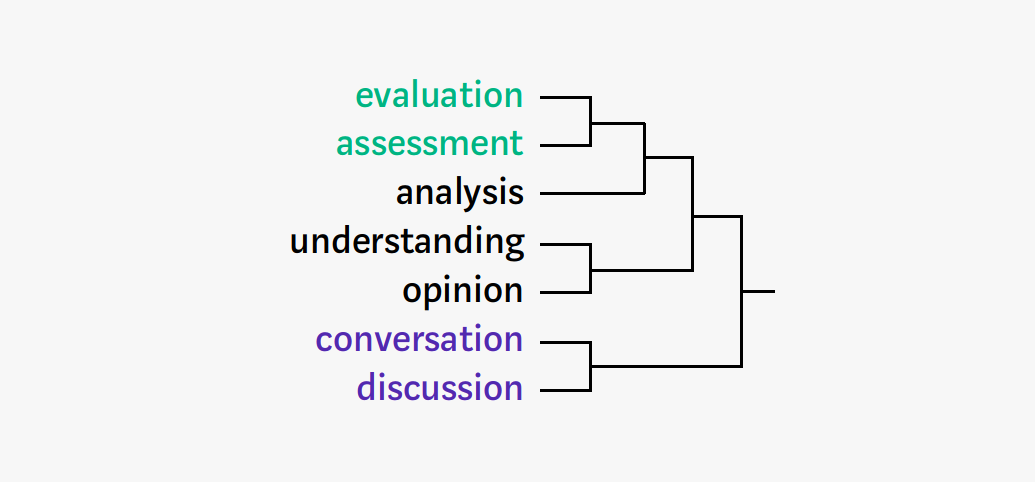
\includegraphics[scale=0.4]{figures/BrownClustering.png}
  \caption{Illustration of a dendogram from Brown Clustering. Adapted from \cite{Brown1992}}
  \label{fig:brownclustering}
\end{figure}

Brown clustering \cite{Brown1992} is an instance of the agglomerative hierarchical clustering algorithm. It uses mutual information based on distributional similarity to place similar words in the same cluster and similar clusters nearby in a binary tree \cite{Derczynski2015}. In practice, Brown clustering takes an input corpus $T$ and number of classes $K$, and uses mutual information to assign each term in the corpus vocabulary $V$ to one of the $K$ classes. Ideally, each class contains highly semantically-related words, by virtue of words being distributed according to their meaning. In the main implementation of Brown clustering \cite{Liang2005}, mutual information is measured at the bigram level. 

Brown clustering is a greedy algorithm. Its high computational complexity, together with a lack of efficient implementations, limits its applicability in NLP \cite{ciosici2020}. In addition, Brown clustering essentially works at the word-level and there is no known adaption to phrases.



\paragraph{Self-Organizing Map:}
%[What is it?] 
Self-organizing map (SOM) is an unsupervised learning technique that map multidimensional data onto lower dimensional subspaces via a neural network. First proposed in 1982 by Kohonen \cite{Kohonen1982,Kohonen2001}, it is also known as the Kohonen network. Often used as a data visualization technique, SOM takes $n$-dimensional input data and outputs a two-dimensional map, which resembles a landscape where regions can be interpreted as clusters and the geometric closeness between clusters also indicates their similarity.
 
%[What’s the procedure?] 
A simple SOM is essentially a feed-forward neural network trained with a competitive learning algorithm. Typically, it consists of a two-dimensional grid of nodes. Each node is initialized to be a randomly-generated weight vector of the same dimensions as the input data. During training, an input is presented to the network, and the node that is most similar to this input is selected to be the 'winner'. The winning node is then updated towards the input vector under consideration. Other nodes in the neighborhood are also influenced by the input vector in a similar manner, but as a function of their topological distance to the winner. The final output of a SOM is such that adjacent nodes have a greater degree of similarity to each other in comparison to nodes that are far apart. In this way, the SOM extracts the latent structure of the input space.

An illustration of the SOM with a two-dimensional grid view is provided in Figure \ref{fig:SOM}. The steps of the SOM learning algorithm are as follows:

\begin{enumerate}
  	\item \emph{Initialize:} Select the grid size (i.e., $X \times Y$), topology (e.g., rectangular), neighborhood function (e.g., Gaussian) and learning rate; each neuron is initialized with a random weight vector that has the same dimension as the input data. 
	\item \emph{Sample:} Select an input data point at random and feed it into the SOM.
	\item \emph{Match:} Find the Best Matching Unit (BMU), which is the neuron with the weight vector most similar to the input data. The similarity measure is usually based on Euclidean distance. 
	\item \emph{Update:} Adjust the weight vectors of the BMU and its neighboring neurons to be closer to the input data according to the preset neighborhood function and learning rate.
	\item Repeat steps 2 - 4 until the neuron weights stabilize.
\end{enumerate}


\begin{figure}[h!]
\centering
  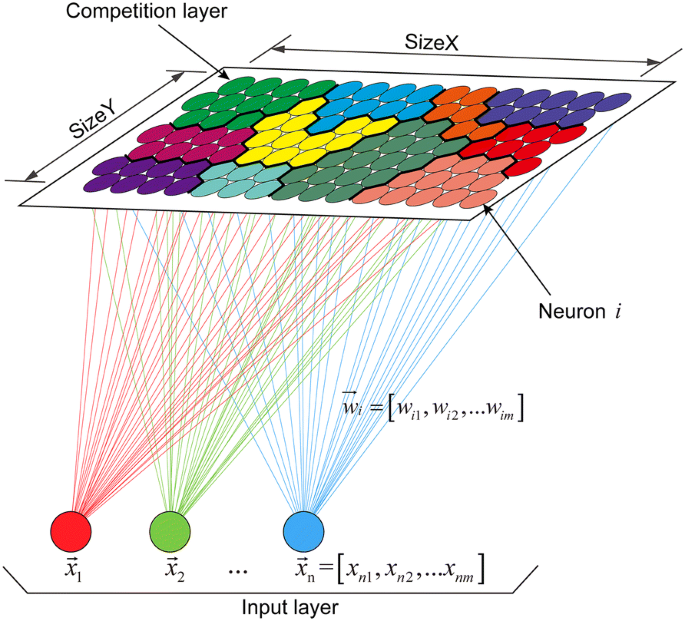
\includegraphics[scale=0.4]{figures/SOM_1.png}
  \caption{Illustration of a SOM. Adopted from \cite{Han2019}}
  \label{fig:SOM}
\end{figure}


%[add evaluation measures of SOM]
Kohonen originally suggested to use quantization error (QE) as the basic quality measure for evaluating SOMs \cite{Kohonen2001}. It is a measure of the average distance between the data points and the map nodes to which they are mapped, with smaller values indicating a better fit \cite{SOM2017}. The QE value for a SOM model is calculated using Equation \ref{qe}, where $n$ is the number of data points in the training data and $\phi : D \rightarrow M$ is the mapping from the input
space $D$ to the SOM $M$:

\begin{equation}\label{qe}
QE(M) = \frac{1}{n} \sum_{i=1}^{n} || \phi (x_i) - x_i||
\end{equation}

Topographic error (TE), on the other hand, is a measure of how well the structure of the input space is modeled by the map. It accounts for a SOM's preservation of local topological features in a low dimensional output space \cite{SOM2017}. Specifically, it is calculated according to Equation \ref{tp} by finding the best-matching and second-best-matching neurons in the map for each input and then evaluating their positions. If the nodes are next to each other, then topology is deemed to have been preserved for this input. If not, then this is counted as an error. The total number of errors divided by the total number of data points gives the topographic error of the map.  

\begin{equation}\label{tp}
TE(M) = \frac{1}{n} \sum_{i=1}^{n} t(x_i)
\end{equation}

where $t(x) = 0$ if the best matching and second best matching neurons are neighbors; else $t(x) = 1$.

% In each epoch, the SOM model is updated the same number of iterations as the number of data points in the training set, as the model is presented with only one data point in each iteration. As shown in Figure \ref{fig:epoch}, we find that increasing number of epochs (i.e. number of times that the model is trained on the entire dataset) does not affect the quantization error and the topographic error.


%[Limitations and applications] 
SOM has a few limitations. One drawback is that unlike other cluster methods, it has no distinct cluster boundaries. When datasets become more complex it is not easy to distinguish the cluster by pure visualization \cite{SOM2016casestudy}. SOM also suffers from the following problem: the network structure including the topology and the number of units has to be set before training and different structures lead to different results \cite{SOM2003}. 

%Evaluation of clustering: 
Clustering remains as a difficult problem in a number of application domains. This can be attributed to the inherent vagueness in the definition of a cluster, and the difficulty in defining an appropriate similarity measure and objective function \cite{Jain2010}. Ideally, clusters are isolated and compact. In reality, the determination of a good cluster is subjective and depends on its end application. Its significance and interpretation often requires domain knowledge. However, while humans are excellent cluster identifiers in two to three dimensions, automatic algorithms are needed to process higher dimensional data \cite{Xu2015Survey}. 



\section{Text Mining in Financial Reports}\label{sec:financial}

\subsection{SEC Regulation} \label{subsec:SEC}

% [SEC regulation and financial documents format 1 page]
The Securities and Exchange Commission (SEC) is the regulatory body in the United States whose mission is to facilitate a fair, efficient and transparent market. The SEC requires all publicly-listed firms in the U.S. to comply with certain disclosure requirements. This information is published in electronic form through the Electronic Data Gathering, Analysis and Retrieval System (EDGAR). EDGAR is a public database offering free access to professional and retail investors alike to research a public company's financial information and operations by reviewing the filings the company makes with the SEC. The system processes about 3,000 filings per day, serves up 3,000 terabytes of data to the public annually, and accommodates 40,000 new filers per year on average.\footnote {https://www.sec.gov/edgar/about} 

The sheer volume and frequency of information uploaded to EDGAR makes it impossible for human experts to manually scrutinize all available and potentially relevant content. Unsurprisingly, practitioners increasingly turn to technological solutions for assistance. However, automatic information extraction is a challenging task for machines due to the myriad filing forms and heterogeneity of file types. With a list of over 150 filing forms, EDGAR contains thousands of document types, both structured and unstructured, across many file formats such as HTML, PDF, plain text, PowerPoint, event pictures, images, etc. \cite{OpenEDGAR2008}.

The SEC has made a number of changes to its file format requirements since its founding in 1933. Its electronic repository dates back to 1984. As a result of this long history, there are no consistent file types even for the same type of forms in the EDGAR database. For example, SEC has initiated the eXtensible Business Reporting Language (XBRL) for the EDGAR database in 2005, in order to facilitate automated information extraction. In XBRL, filers tag their financial statements with elements from a taxonomy that defines the reporting concepts so that the accounting numbers are linked and can be collected automatically. Early adoption of XBRL by companies was gradual, but it was finally made mandatory in 2014. In 2018, the SEC adopted new rules requiring financial information to be submitted in the Inline XBRL format. Inline XBRL is a specification of XBRL that is both human-readable and machine-readable.\footnote {https://www.sec.gov/page/osdhistoryandrulemaking} 

Furthermore, companies have considerable flexibility in changing the tagging, wording, and presentation of these documents as long as they follow a predefined reporting structure. Loughran et al.~\cite{Loughran2016} pointed out a few issues, for instance, the 10-K filings are far less structured prior to about 2002 and many times a segment is mislabelled or misspelled. As a result, what seems like an obvious segmentation of the document, computationally is not. In addition, the same types of SEC filings may vary significantly between companies and over time, prohibiting researchers, regulators, and even many well-equipped practitioners from utilizing automation to extract information \cite{lazyprices2020}.

Despite these challenges, corporate disclosures on EDGAR are still a very important data resource for academic research, especially for longitudinal studies that requires historical data going back many decades. With regards to studies in Finance and Accounting, many recent survey papers have pointed out that the most commonly used datasets for text mining analyses are annual reports (Form 10-K) and quarterly reports (Form 10-Q) \cite{Tueregun2019, Gupta2020, Ravula2020}. In particular, within these 10-K and 10-Q filings, the Management Discussion and Analysis (MD\&A) sections are the focal point for many studies.

\subsection{Management Discussion and Analysis}

MD\&A is a narrative explanation of the financial statements and other statistical data that the registrant believes will enhance a readers' understanding of its financial condition, changes in financial condition and results of operation\footnote{https://www.sec.gov/corpfin/cf-manual/topic-9}. The SEC and the International Accounting Standards Board (IASB) insist on providing meaningful causal explanations and related discussions of performance results in management commentary.

The SEC specifically requires that the MD\&A section "should not consist merely of numeric dollar and percentage changes measured from period to period. [...] The focus should be on an analysis of the factors that caused these changes to occur."\footnote {https://www.sec.gov/corpfin/cf-manual/topic-9} For example, if sales declined because the volume of goods sold decreased by 20\%, but this was offset by a 10\% increase in price, the discussion in MD\&A should not stop once it identifies the price and volume components. In this example, the underlying factors that contributed to the decline in volume as well as the increase in selling prices should also be discussed. It is further suggested that for events that are likely to cause a material change in the relationship between costs and revenues (e.g., increases in labor costs or raw materials), the change in the relationship should be disclosed.
 
In its Practice Statement, the IASB (2010)\footnote {https://www.ifrs.org/issued-standards/list-of-standards/management-commentary-practice-statement/} voices similar arguments. Firms should use management commentary to include their own perspective on how their business is evolving with an analysis of how different factors are interacting to assist market participants in interpreting the financial statements and in comprehending their content in relation to management's objectives and strategies and action to achieve those objectives. Causal reasoning about performance is imperative in this respect \cite{Zhang2018}.

There are many studies focused on MD\&A, though causality-related research is rare. Clarkson et al.~\cite{clarkson1998} present evidence regarding the usefulness of MD\&A. and on disclosure quality. Numerous research analyzes MD\&A to explain a company's M\&A strategy (\cite{Ahmed2016}), future earnings and profitability (\cite{Feldman2010, Bochkay2014, AmelZadeh2016}), stock performance (\cite{AmelZadeh2016, TaoDeokar2018}), bankruptcy and litigation risks etc. (\cite{YangDollarMo18, BourveauLouWang18}). Most of these studies focus on basic and simple indicators such as readability, FOG index, tone and sentiment analysis, in combination with regularized regression methods to explain correlation between a company's attributes and its financial disclosure. Ravula \cite{Ravula2020} provides a very comprehensive summary of all latest research in this field and points out that text analysis in finance is still in the early stages.

Separately, MD\&A has also been used as a domain specific corpus to train language models. FinBERT \cite{finBERT2020} obtains 60,490 Forms 10-K and 142,622 Forms 10-Q of Russell 3000 firms for 1994 to 2019 from the SEC's EDGAR website. 

%There are also knowledge graph construction related studies. Such as company holdings, management employment, competitor analysis, etc. [add reference]


% TODO
\section{Related Work} \label{sec:related}
Most of the works mentioned in the previous sections of this chapter are relevant to this thesis. In this section, we highlight a select few that are the most relevant. They all use financial filings as their main corpra to extract information. 

Zhang et al.~\cite{Zhang2018} use automated techniques to measure causal reasoning on earnings-related financial outcomes of a large sample of MD\&A sections of US firms. They find a positive and significant correlation between a company's causal reasoning intensity and the earnings forecast accuracy by analysts following the company. One limiation of this study is that they use a rather simplistic approach to measure the causal reasoning word intensity, i.e., by counting the relative frequency of causal reasoning words in the performance-related paragraphs of the MD\&A. The identification of the causal reasoning words is based on a list of causal words used by Linguistic Inquiry and Word Count (LIWC). 

Chen et al.~\cite{Chen20} use financial statements as the corpus to extract nested causality. They propose to train a joint model consisting of two layers of Bi-LSTMs end to end based on the annotated dataset. Their model is capable of finding nested causality structure in a sentence. The first layer of the model separate a sentence into segments and the hidden state of each segment is fed into the second bi-directional LSTM layer, which classifies whether there exists a causal relation between all pairs of segments within the sentence. To train this neural network, significant effort is required to prepare the data for manual annotation. In their case, a team of 25 volunteers participated in the annotation task. They manually collected and annotated 69,120 sentences from 2,039 published financial documents. Unfortunately, neither the source of the financial documents nor the language of these documents is specified in the paper. Another limiation is that the authors did not make this annotated dataset publicly available, thus it cannot be used as a training set for this theisis. 

Cavar and Josefy \cite{MappingKG2018} uterlize NLP techniques to extract information from SEC filings and construct a knowledge graph of how companies, their executives and directors are linked to one another. Their graph-mapping approach includes extracting subject-predicate-object tuples from raw text and validating the semantic relations through linguistic analyses. However, due to the lack of a gold standard corpus or data set, the authors did not provide any formal and quantitative measure for the effectiveness of their extraction pipeline. In addition, another limiation is that this paper does not provide any overview of statistics on the final knowledge graph constructed, or how it can be used in downstream applications. 

Jen \cite{CompanyKG2021} constructs a company domain-specific knowledge graph that contains company-related entities and relationships, such as competitiors, subsiddiearies, suppliers and custerms, from 10-K filings. This project applies hybrid methods combining a pre-trained statistical model for NER and rule-based patterns for RE. To evaluate the proposed model's performance, the author manually gathers all the available triples based on the ontology schema from 10-K filings as a gold standard. Ten 10-K filings are used to create rule-based patterns and the system's performance is evaluated on another ten 10-K filings. A precision of  75.7\% and a recall of 53.6\% are achieved by the proposed system. As the data source only includes 20 filings, the scope of this project is rather limited. In addition, there is also no evaluation on possible end applications using the company domain-secific knowledge graph created. 

In addition to the works related to information extraction from financial documents, this thesis also borrows inspiration from the following paper, in terms of output visualiazation. Skupin et al.~\cite{SOM2013} implement a high-resolution visualization of the medical knowledge domain using the self-organizing map method, based on a corpus of over two million publications. They use a basic vector space model with a vocabulary consisting of only the top 10\%, or 2,300 most used MeSH terms (PubMed Medical Subject Headings) in conjunction with a large SOM consisting of over 75,000 neurons. After training, a neuron label clustering method is applied to merge boundaries and determine cluster labels. The resulting map is further annotated and evaluated by ten experts stemming from the biomedical domain. This study produces some very interesting visualization as output and concludes that it is possible to transform a very large document corpus into a map that is visually engaging and conceptually stimulating to subject experts.









\newpage

%%%%%%%%%%%%%%%%%%%%%%%%%%%%%%%%%%%%%%%%%%%%%%%%%%%%%%%%%%%%

\chapter{A Network of Causal Factors} \label{conceptualization}

%\chapter{Conceptual Framework} \label{conceptualization}

In this chapter, we specify the conceptual framework of a graph-based data model that represents the causal factors that drive the financial performances of S\&P 500 companies. We also provide some general computational approaches for solving the problems stated in Chapter \ref{introduction}. We start with an overview of the key objectives in Section \ref{sec:overview}, followed by a brief discussion on causal factor representation in Section \ref{sec:causalrepresenation}. In Section \ref{sec:datamodel}, we present a detailed description of the data model as well as a discussion on its key characteriscs. In Section \ref{sec:similarity}, we introduce similarity measures and algorithms to be performed on the data model. Finally, in section \ref{sec:queries}, we showcase some potential queries and the expected outputs from the data model.


\section{Overview and Objectives} \label{sec:overview} 

As mentioned in Chapter \ref{introduction}, the primary motivation for this thesis is to create a text mining system that can be utilized to deal with practical problems encountered in investment research by mining the financial reports. A key set of the fundamental research questions concerns about companies' business models and the underlying industry trends. Some specific questions that investment analysts need to address often include:

\begin{itemize}
\item	What factors affect a particular company's financial performances? 
\item	How do these factors generally change with time? Is there any recognizable pattern?
\item     Which are the most closely related and comparable peers of a company?
\item	Given certain macro-level events, e.g., geopolitical conflicts, food price inflation, and interest rate hikes, etc., which companies are more likely to be affected?
\end{itemize}

For the purpose of this thesis, \emph{causal factors} are defined as a set of specific events, a general economic phenomon, or a category of business activities, etc., which impact the financial performance of a company or a group of companies for a defined period of time. Some example of causal factors include: increase ind paid subscribers, impact of Covid-19 pandemic,  performance-based compensation, headcount increase, etc.. These causal factors are meant to cover a broad variety of contents as well as a wide range of granuality. They are allowed to be as specific or as general as possible. The intention is to capture not only the immediate, direct drivers of specific financial metrics, but also the implicit root cause of certain shifts in financial performance over the long run. 

Understanding these causal factors helps investors to forecast the future performance of companies under different scenarios, in order to evaluate their intrinsic worth. By comparing a company's relative value with its comparable peers in the same or related sector, it leads eventually to the identification of better investment candidates, value arbitrage opportunities as well as interesting thematic investment strategies. 

Answers to most of these question can be found in the financial reports, however, they do not exist in a readily available form that can be directly retrieved via keyword search. These answers have to be synthesized through incorporation of relevant information, abstraction and summarization. To design a system that can explicitly address these questions by mining information from financial reports, we take inspiration from observing the human analysts' approaches and attempt to infuse as much expert knowledge as possible in our system. 

The \textbf{first observation} is that an experienced analyst usually knows where to look for the relevant information in the financial reports. Instead of the most naive approach of reading a financial report in its entirety in a linear fashion, he or she can quickly locate the specific sections to focus on, based on reasonable expectation of the report's structure and prior knowledge. Moreover, within the relevant section, an analyst also pays more attention to the sentences that explicitly express credit attribution in order to extract useful information. For example, a sentence such as \emph{"There was an increase in operating expenses primarily driven by an increase in compensation expenses largely due to increases in headcount."} is where the analyst would be focused on, if he or she is primarily interested in finding out what causal factors affect the \emph{operationg expenses}. In this example sentence, the causal explanation associated with the effect of \emph{"increase in operation expense"} can be attributed to the explicit factors such as \emph{"an increase in compensation expenses"} and \emph{"increases in headcount"}. We would like our system to incorporate these heuristic rules to facilitate in the information extraction process.

The \textbf{second observation} is that human naturally processes information by abstraction and association with similar concepts. Once a causal factor that affects the financial performance of a company is identified, the analyst is able to categorize it with other similar causal factors of the other companies. As they accumulate such a web of the associative knowledge throughout the years, they develop a so-called business intuition on which companies are affected by similar or related causal factors and in what ways. Therefore we need a representation of these causal factors which enables our system to perform similar tasks of abstraction and association. In other words, our system need to be able to cluster these causal factors into meaningful groups that could help with pattern discovery.

The \textbf{third observation} is the dynamic nature and the interwoven complexity in the company-factor relation patterns. We know from experience that some causal factors are company-specific, while others might be generic and shared among many companies at a macro-level. In addition, some factors might be related to an one-off event, yet other times they could be recurring or cyclical in nature. Furthermore, it is also essential that our data model is dynamical in nature and capable of adapting to new patterns. The performance factors evolve with time, hence, the data model needs to be updated incrementally when new information becomes available.
  
To derive such a data model with these specific requirements as discussed above, we need a two-staged approach. Firstly, all the causal factors driving the financial performance are to be extracted from the raw texts of individual companies. Next, the extracted factors are further processed via clustering algorithms. In addition, the data model should be accessed and queried by a user to retrieve data and output a visualization. Figure \ref{fig:pipeline} illustrates the envisioned data processing pipeline to achieve this purpose.  

\begin{figure}[h!]
\centering
  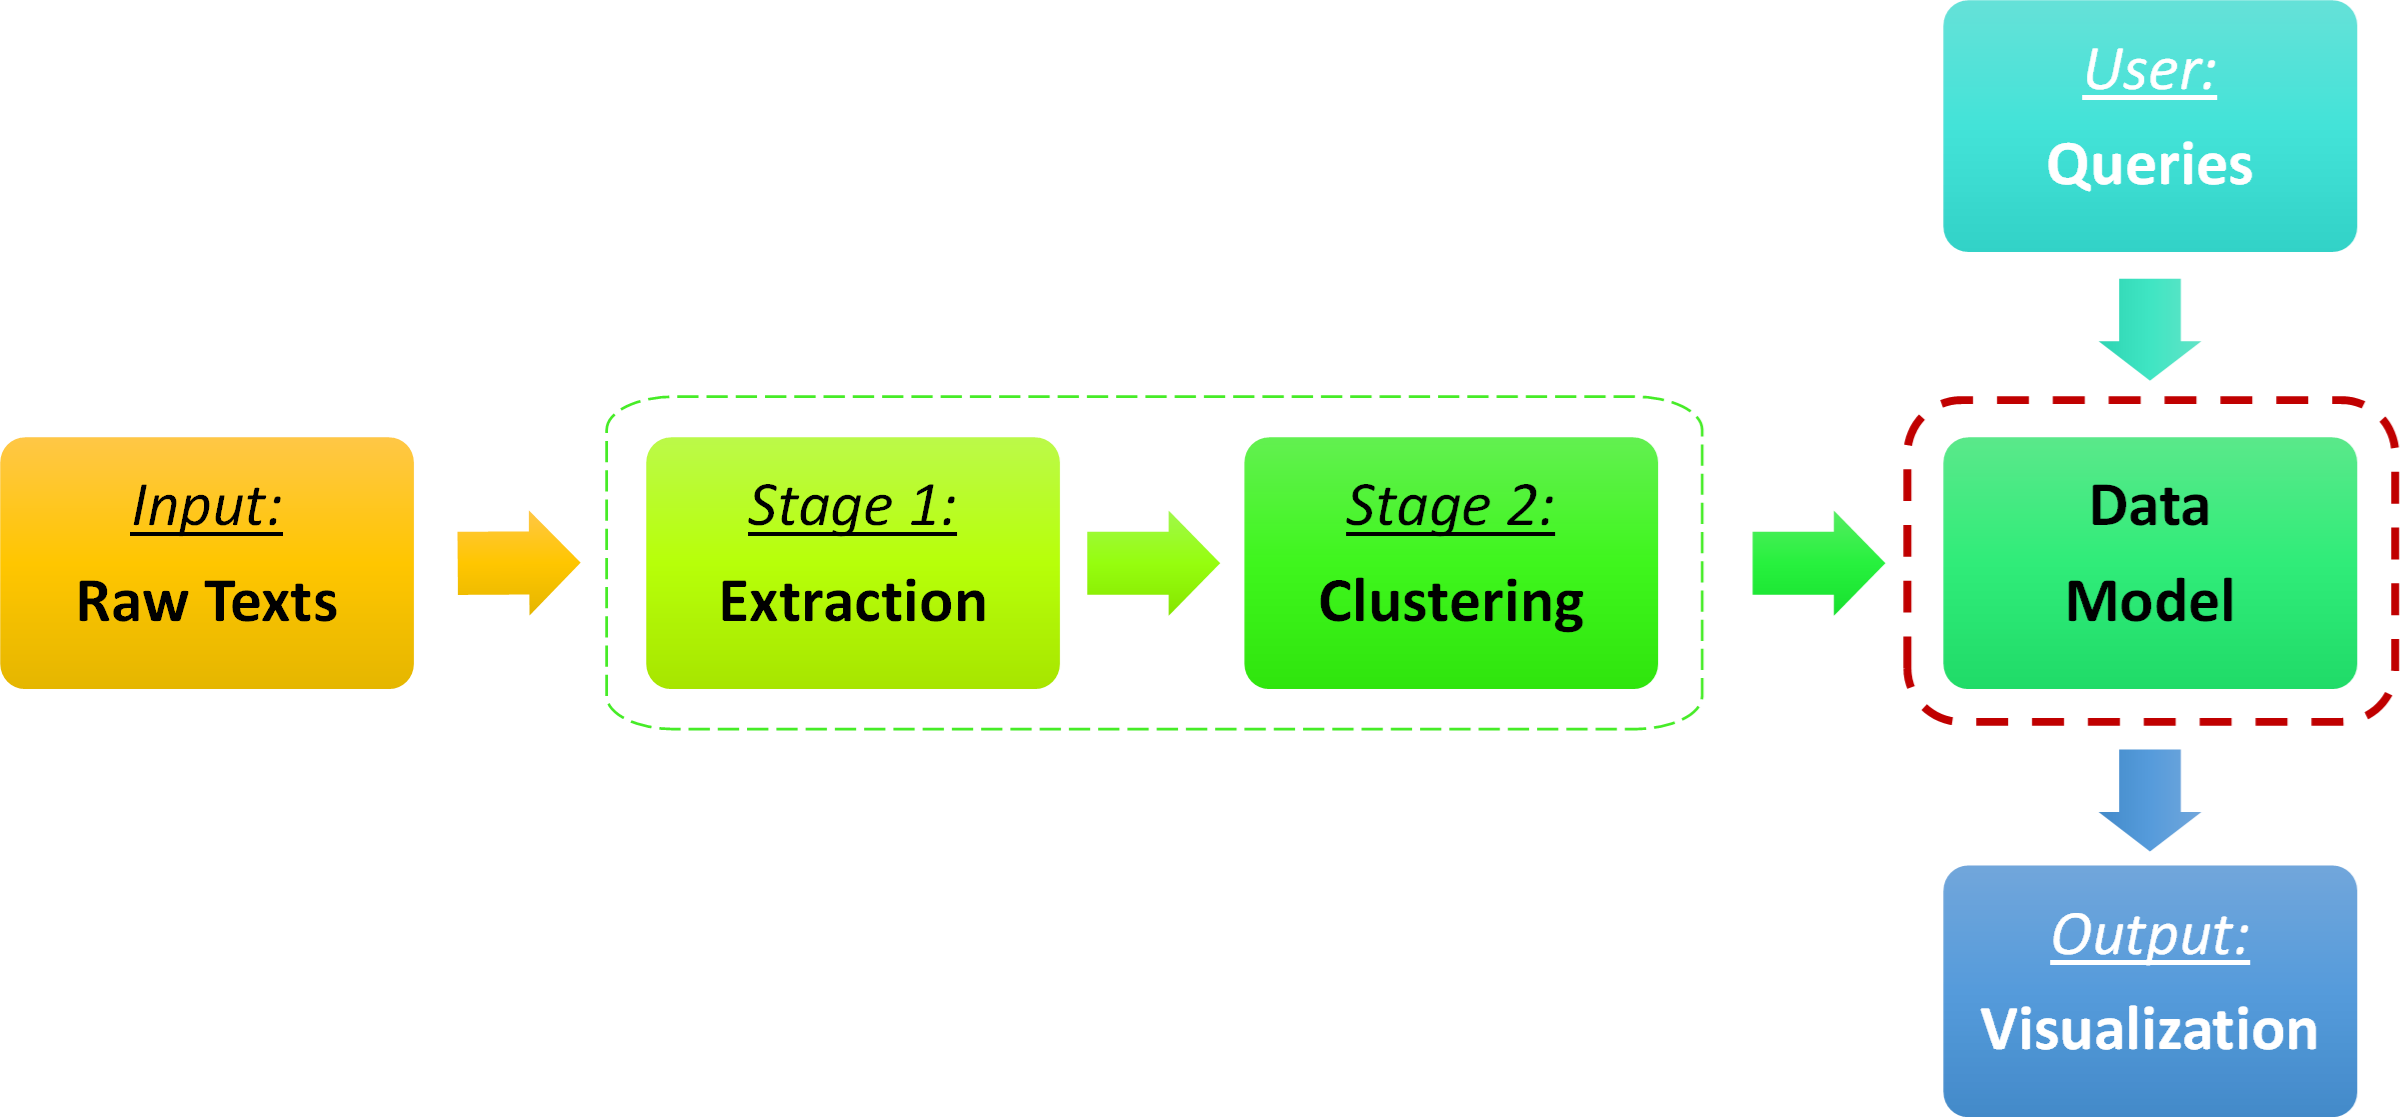
\includegraphics[scale=1.4]{figures/Pipeline_0.png}
  \caption{Illustration of Data Processing Pipeline}
  \label{fig:pipeline}
\end{figure}



\section{Representation of Causal Factors} \label{sec:causalrepresenation}

In this section, we first establish a common understanding on identification of casual sentences. We illustrate our approach in terms of cause and effect chunks in this context. We also discuss the representation of causal factors in terms of concept clusters. 

\subsection{Causal Sentences}
For the purpose of performing the extraction task in our system, a causal sentence is defined as a sentence that contains three components: a cause (C), an effect (E) and an explicit causal connector (CC). A cause is a text fragment within a sentence that describes an event or phenomenon that causes another event or phenomena, i.e., the effect. These cause and effect text fragments can be a word, a phrase or a clause. 

A causal connector is a linguistic signal of causality and it can be in the form of a verb (e.g., E driven by C), a preposition phrase (e.g., E due to C), a conjunction (e.g., E because C), etc. The causal connector can be used as a marker to segment a causal sentence into chunks of text fragments corresponding to cause and effect, respectively. For example, the causal sentence, "The increase in operating expenses was primarily driven by an increase in sales and marketing cost.", can be presented as: E = "the increase in operating expenses", connector = "driven by", C = "an increase in sales and marketing cost". Any causal sentence can be represented as one of the two patterns of cause-effect chunks linked by causal connectors, as illustrated by Figure \ref{fig:blockpatterns}.  


\begin{figure}[h!]
\centering
  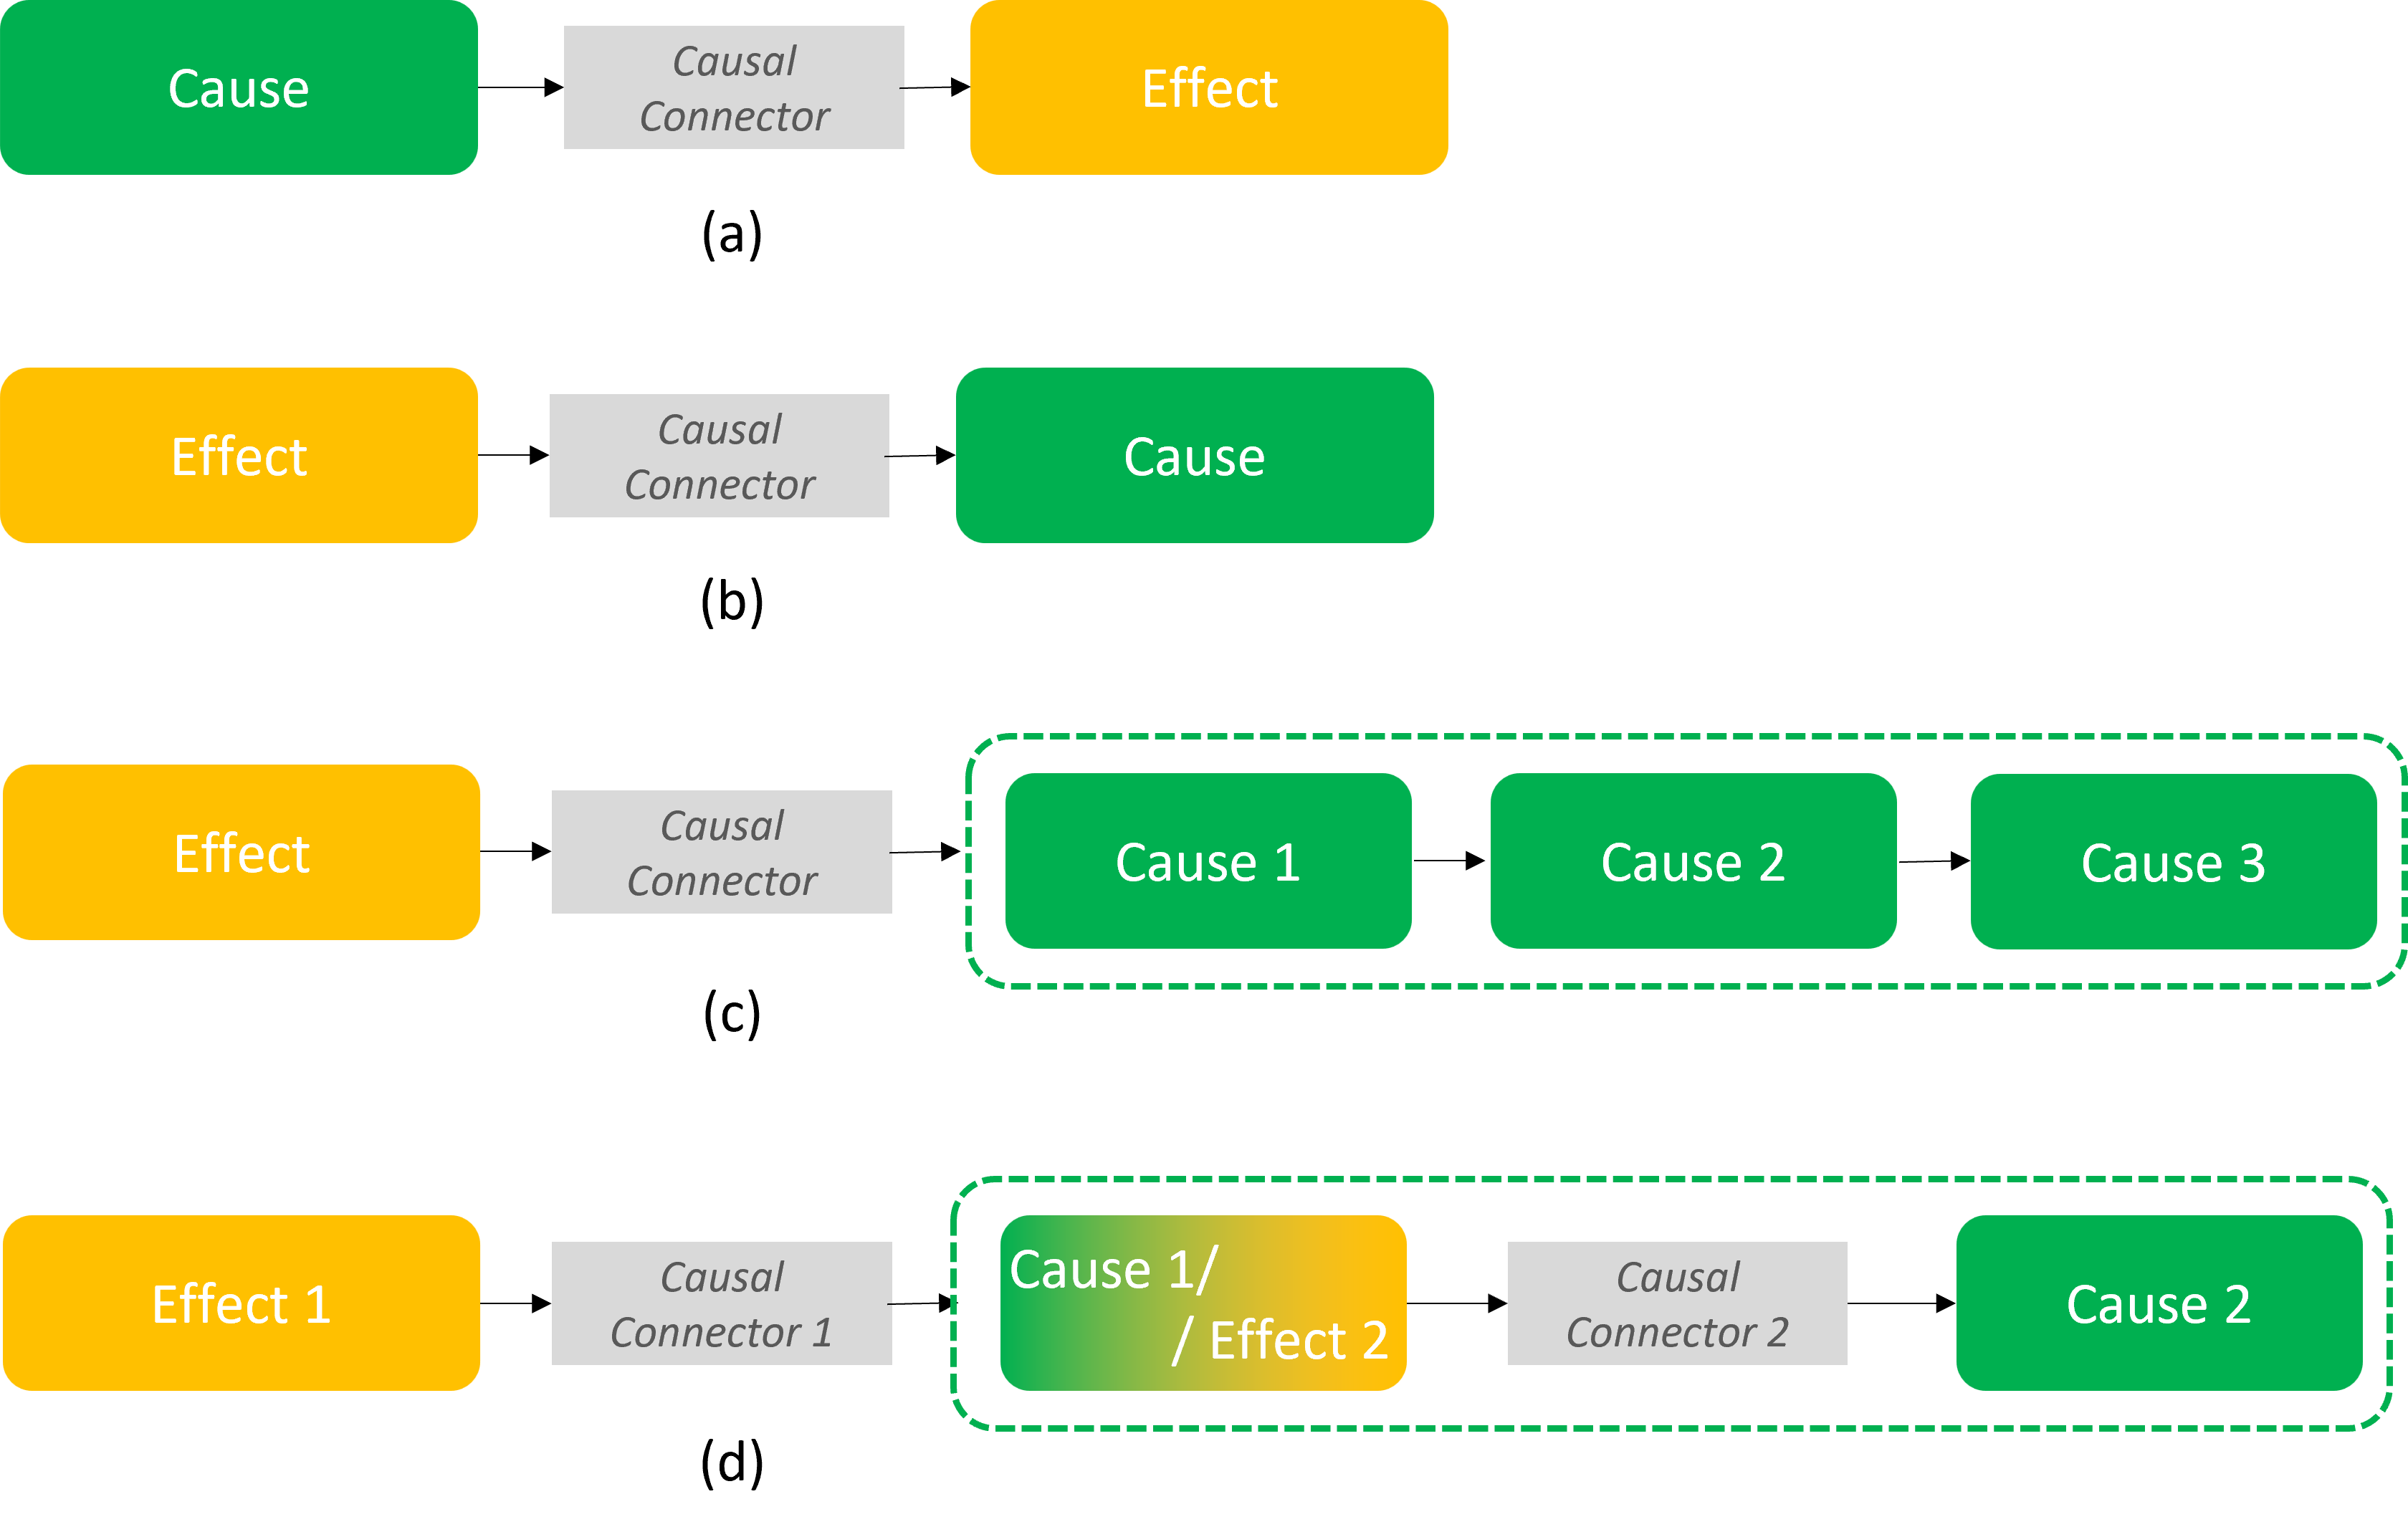
\includegraphics[scale=0.5]{figures/CausalBlocks.png}
  \caption{Illustration of typical patterns in causal sentences. (a) and (b) are patterns of simple causal sentences that involves only a single pair of cause and effect event; (c) represents a compound causal sentence with a single effect and multiple causes; (d) represents a compound causal sentence with two causal connectors. In both cases (c) and (d), our system treats the complex causes as a combined chunk.}
  \label{fig:blockpatterns}
\end{figure}


Depending on the part-of-speech function of the causal connector, as well as the complexity of the corresponding cause and effect chunks, the causal sentence can have a simple, compound or complex sentence structure. For example, a causal sentence such as \emph{"Growth for our direct response advertising products was primarily driven by increased advertiser spending as well as improvements to ad formats and delivery."}, contains multiple causes attributing to one single effect, E = \emph{Growth for our direct response advertising products}, C1 =\emph{increased advertiser spending}, C2 =\emph{improvements to ad formats and delivery}. In this case, our system treats C1 and C2 as one combined cause chunk. Another example, in the sentence \emph{"There was an increase in operating expenses primarily driven by an increase in compensation expenses largely due to increases in headcount"}, there is a causal chain with multiple causal connectors (\emph{"driven by", "due to"}). In theory, this causal sentence can be broken down into two subsets of cause-effect chunks: 1) E1 = \emph{an increase in operating expenses}, C1= \emph{an increase in compensation expenses}; 2) E2 = \emph{an increase in compensation expenses}, C2 = \emph{increases in headcount}. However, in this case, our system treats C1 and C2 as a combined cause chunk. See illustration in Figure \ref{fig:blockpatterns}.  

%[justification for this simplification]. 
In the context of financial reports, managements explain about the company's financial performances in a business formal language that is logical, concise and unambiguous. As a result, the causal sentences typically have an effect chunk refering to a change in one particular financial metric, for example, growth in revenue, decline in gross profit, improvement in EBITDA margin, decrease in net income, etc. A \emph{topic} is defined as a financial metric term that is expressed in an effect chunk of a causal sentence. Specifically, the \emph{topics} referred to in the above examples are \emph{revenue, gross profit, EBITDA margin} and \emph{net income}.


\subsection{Causal Factors}
The cause chunk in a causal sentence typically express the explanation of factors that affect a business' financial performance, which our system is tasked to extract and analyze. There factors are referred as \emph{Causal Factors}. There are various way of representing these causal factors. 

The most naive way is to treat each cause chunk as one cause factor and store the original text fragments in a database which can be searched via key words. To compare similarities amongst these factors, a bag-of-words or TFIDF approach could be applied. However, the key limitations of this approach is that it ignores the structure and semantic information embedded in text fragments and the weight of each term only reflects the term frequency rather than the functional role in a sentence. In addition, the size of vocabulary as the dimension of the vector representation resulting in sparse data in a high-dimensional space, which is computationally inefficient to deal with.  

Another approach is to represent these factors as events with a template specifying a set of pre-defined features, such as time, location, actor, movement, etc. The advantage is to have a controllable number of features. However, this slot-filling approach requires a lot of expert input in order to manually handcraft. The factors could be diverse and therefore difficult to design a template that fits all scenarios.   

Taking inspiration from both of the above mentioned methods, we adopt the following approach: a cause chunk is represented as a directed graph, where the vertices are the noun phrases in the text fragment and the directed edges represents the connecting texts that are in between those noun phrases. The connecting text could be a verb, a conjunction, part of a preposition phrase, etc.. 

In this model, the noun phrases are treated as carriers of concepts and the connection texts as indication of relationships between these concepts. These noun phrases are further clustered into groups based on semantic similarities. In other words, we group synonyms or phrases representing similar concepts into the same cluster. Ideally, a concept can be identified from each cluster of noun phrases. These clusters can also be considered as equivalent to the slots in a template, except these features are automatically generated based on unsupervised learning rather than manually defined by expert beforehand. 

Replacing each noun phrase with its corresponding concept cluster that it belongs to, each cause chunk can therefore be represented as a sequence of connected concept clusters in the direct graph. Instead of using each unique noun phrase as a feature, we use these concept clusters as feature space, thus effectively reducing the dimensionality of feature space to represent these factors. 

Alternatively, we could use a language model such as BERT to obtain the contextualized embeddings for these text fragments, however, this black-box approach is not interpretable. 




\section{Data Model} \label{sec:datamodel}

In this section, we describe our data model in details. We first establish the data model as a heterogenous graph, then elaborate on the specification for each node type and how the data model is built step by step. We also discuss the key characteristics of the data model. 

\subsection{Node and Edges}

In essence, our data model is a heterogeneous graph $\mathbf{G} = (\mathbf{V}, \mathbf{E})$ with five distinct node types: \emph{Company}, \emph{Document}, \emph{CausalSentence}, \emph{NounPhrase}, and \emph{Concept}.
\[\mathbf{V} = \mathbf{V}_{company} \cup \mathbf{V}_{document} \cup \mathbf{V}_{causalSentence} \cup \mathbf{V}_{nounPhrase} \cup \mathbf{V}_{concept} \]

There exists a natural order of hierarchy among these nodes, which is indicated by the four distinct types of directed edges:
\[\mathbf{E} = \mathbf{E}_1 \cup \mathbf{E}_2 \cup \mathbf{E}_3 \cup \mathbf{E}_4 \] where 
\[\mathbf{E}_1 \subseteq \mathbf{V}_{company} \times \mathbf{V}_{document} \]
\[\mathbf{E}_2 \subseteq \mathbf{V}_{document} \times \mathbf{V}_{causalSentence} \]
\[\mathbf{E}_3 \subseteq \mathbf{V}_{causalSentence} \times \mathbf{V}_{nounPhrase} \]
\[\mathbf{E}_4 \subseteq \mathbf{V}_{nounPhrase} \times \mathbf{V}_{concept} \]


We now elaborate on the specification for each node type and the associated edges. We use $(...)$ to denote \emph{nodes}, $-[...]\rightarrow$ to denote \emph{edges} and \{...\} to denote edge properties.


\paragraph{Company Nodes:} Company nodes ($\mathbf{V}_{company}$) represent a set of companies, $\mathcal{C}$, where $\mathbf{V}_{company} \subseteq \mathbf{\mathcal{C}}$. Each company node is identifiable by a unique ticker. Additional node properties include the company's full name and its sector classification. For example, Alphabet Inc. is represented as a company node with the ticker \emph{GOOGL}, company name \emph{Alphabet Inc.} and sector classification \emph{Communication Services}.  


\paragraph{Document Nodes:} Document nodes ($\mathbf{V}_{document}$) represent a set of financial documents, $\mathbf{\mathcal{D}}$, where $\mathbf{V}_{document} \subseteq \mathbf{\mathcal{D}}$. In our case, the set of financial documents consist of form 10-Qs and 10-Ks (see Section 2.3.1). Each financial document is associated with a particular company identifiable by the same unique ticker, as well as a $timestamp$ corresponding to the document's reporting period.  


\paragraph{Directed Edge from Company Nodes to Document Nodes:} There is a one-to-many relationship from the company set to the document set. Each company can be associated with multiple documents over an extended period of time, whereas each document can only be associated with one company. The company-document relationship is represented by a directed edge, $\mathbf{E}_1 \subseteq \mathbf{V}_{company} \times \mathbf{V}_{document}$, in the graph. For each edge, the $timestamp$ encoding the document's reporting period is specified as an edge property, as illustrated below:
\[( c_i ) - [ e_1 \{timestamp\} ]\rightarrow ( d_j ) \]
where $c_i \in \mathbf{V}_{company}$,  $d_j \in \mathbf{V}_{document}$ and $e_1 \in \mathbf{E}_1$.


\paragraph{CausalSentence Nodes:} CausalSentence nodes ($\mathbf{V}_{causalSentence}$) represent a set of sentences which express causality, $\mathbf{\mathcal{S}}$, where $\mathbf{V}_{causalSentence} \subseteq \mathcal{S}$. In our case, the set of causal sentences are extracted from the set of financial documents $\mathbf{\mathcal{D}}$ through a mapping: 
\[f_{extract-causal}: \mathbf{\mathcal{D}} \rightarrow \mathbf{\mathcal{S}}\] 
where $f_{extract-causal}$ corresponds to the process of extracting causal sentences from the set of financial documents.

As discussed in Section 3.2, causal sentences can be decomposed into cause and effect chunks, and the effect chunks typically describe changes or movements in some financial metrics, such as increase in revenue, decrease in margins, and increase in net income. Therefore each causal sentence can be tagged with a $topic$ which refers to the underlying financial metric reflected in the effect chunk. The typical $topics$ include the most common financial Key Performance Indicators (KPIs) such as: \emph{revenue (or sale), cost (or expense), income (or profit), earnings before interest and taxt (EBIT), gross margin, net margin, etc.}. 


\paragraph{Directed Edge from Document Nodes to CausalSentence Nodes:} There is also a one-to-many relationship from the document set to the causalSentence set, since each causal sentence is only associated with one document but multiple causal sentences can be extracted from the same document. The document-causalSentence relationship is represented by a directed edge, $\mathbf{E}_2 \subseteq \mathbf{V}_{document} \times \mathbf{V}_{causalSentence}$, in the graph. For each edge, the $topic$ identified from the effect chunk of the causal sentence, is listed as an edge property, as illustrated below:
\[( d_j ) - [ e_2 \{topic\} ]\rightarrow ( s_k ) \] 
where $d_j \in \mathbf{V}_{document}$, $s_k \in \mathbf{V}_{causalSentence}$ and $e_2 \in \mathbf{E}_2$.


\paragraph{NounPhrase Nodes:} NounPhrase nodes ($\mathbf{V}_{nounPhrase}$) represent a set of noun phrases, $\mathbf{\mathcal{N}}$, where $\mathbf{V}_{nounPhrase} \subseteq \mathcal{N}$. In our case, the set of noun phrases are extracted from the set of causal sentences $\mathbf{\mathcal{S}}$ through a mapping: 
\[f_{extract-np}: \mathbf{\mathcal{S}} \rightarrow \mathbf{\mathcal{N}}\] 
where $f_{extract-np}$ represents the process of extracting noun phrases from the cause chunks of the causal sentences, as discussed in Section 3.2. For example, the causal sentence \emph{"The increase was primarily driven by <high levels of promotional expense in the first quarter of fiscal 2015, a decrease in SG\&A expenses, and lower supply chain costs>."} contains a cause chunk marked in <...>. This cause chunk can be further segmented into the following noun phrases and represented in an ordered list:
[1. \emph{high levels}, 2. \emph{promotional expense}, 3. \emph{the first quarter}, 4. \emph{a decrease}, 5. \emph{SG\&A expense}, 6. \emph{lower supply chain costs}]
The rational for choosing noun phrases, rather than other part-of-speech terms such as verbs, adjectives, etc., is based on the assumption that noun phrases are the most fundamental symbolic representation of concrete objects as well as abstract ideas, thus a natural choice for the basic lexical unit of concepts.


\paragraph{Directed Edge from CausalSentence Nodes to NounPhrase Nodes:} There is a many-to-many relationship between the causal sentence set and the noun phrase set. A causal sentence can contain multiple noun phrases and a noun phrase can be contained in multiple causal sentences. In addition, the order of the sequence that the noun phrase appear in a causal sentence is also important and must be encoded in the respective relationship. For the same example above, the edge connecting the noun phrase node \emph{high levels} to the sentence node should an $order$ value of 1; the edge associated with \emph{promotional expense} has an $order$ value of 2, etc. and so on for the rest of the nouns in the ordered list. 

Therefore, the relationships from the causal sentence to each of its constituent noun phrases are represented as directed edges, $\mathbf{E}_3 \subseteq \mathbf{V}_{causalSentence} \times \mathbf{V}_{nounPhrase}$. Each edge has a property that corresponds to the $order$ of the noun phrase's appearance in the cause chunk of the causal sentence, as illustrated below:
\[( s_k ) - [ e_3 \{order\} ]\rightarrow ( n_p ) \] 
where $s_k \in \mathbf{V}_{causalSentence}$, $n_p \in \mathbf{V}_{nounPhrase}$ and $e_3 \in \mathbf{E}_3$.


\paragraph{Concept Nodes:} Concept nodes ($\mathbf{V}_{concept}$) represent a set of concepts, $\mathbf{\mathcal{CC}}$, where $\mathbf{V}_{concept} \subseteq \mathcal{CC}$. A $concept$ is defined as an abstract representation of a group of semantically similar noun phrases. In this case, the set of concepts are formed from partitioning the set of noun phrases into a set of clusters, with each cluster representing a concept
\[f_{cluster-np}: \mathbf{\mathcal{N}} \rightarrow \mathbf{\mathcal{CC}}\] 
where $f_{cluster-np}$ represents the hard clustering process of assigning each noun phrase to one particular concept. For example, noun phrases such as \emph{Europe, EU, Middle East, Africa, Asia Pacific, North Americas}, etc. are expected to form a cluster, from which the concept of \emph{continent or region} can be identified.  


\paragraph{Directed Edge from NounPhrase Nodes to Concept Nodes:} There is a many-to-one relationship between the noun phrase set and the concept set. This results directly from the condition of hard clustering: each concept consists of multiple noun phrases, however, each noun phrase can only be clustered into one concept. The relationships between the noun phrase sets and the concept sets are represented by directed edges, $\mathbf{E}_4 \subseteq \mathbf{V}_{nounPhrase} \times \mathbf{V}_{concept}$, in the graph:
\[( n_p ) - [ e_4 \{order\} ]\rightarrow ( cc_q ) \] 
where $n_p \in \mathbf{V}_{nounPhrase}$, $cc_q \in \mathbf{V}_{concept}$ and $e_4 \in \mathbf{E}_4$.
There is a potential to extend this model to soft clustering where the edge can also encode the probability. However, this is beyond the scope of this thesis. 


Figure \ref{fig:AssumpSet} provides a graphical overview of the set relationships among the five distinct node types in the heterogenous graph-based data model.
\begin{figure}[h!]
\centering
  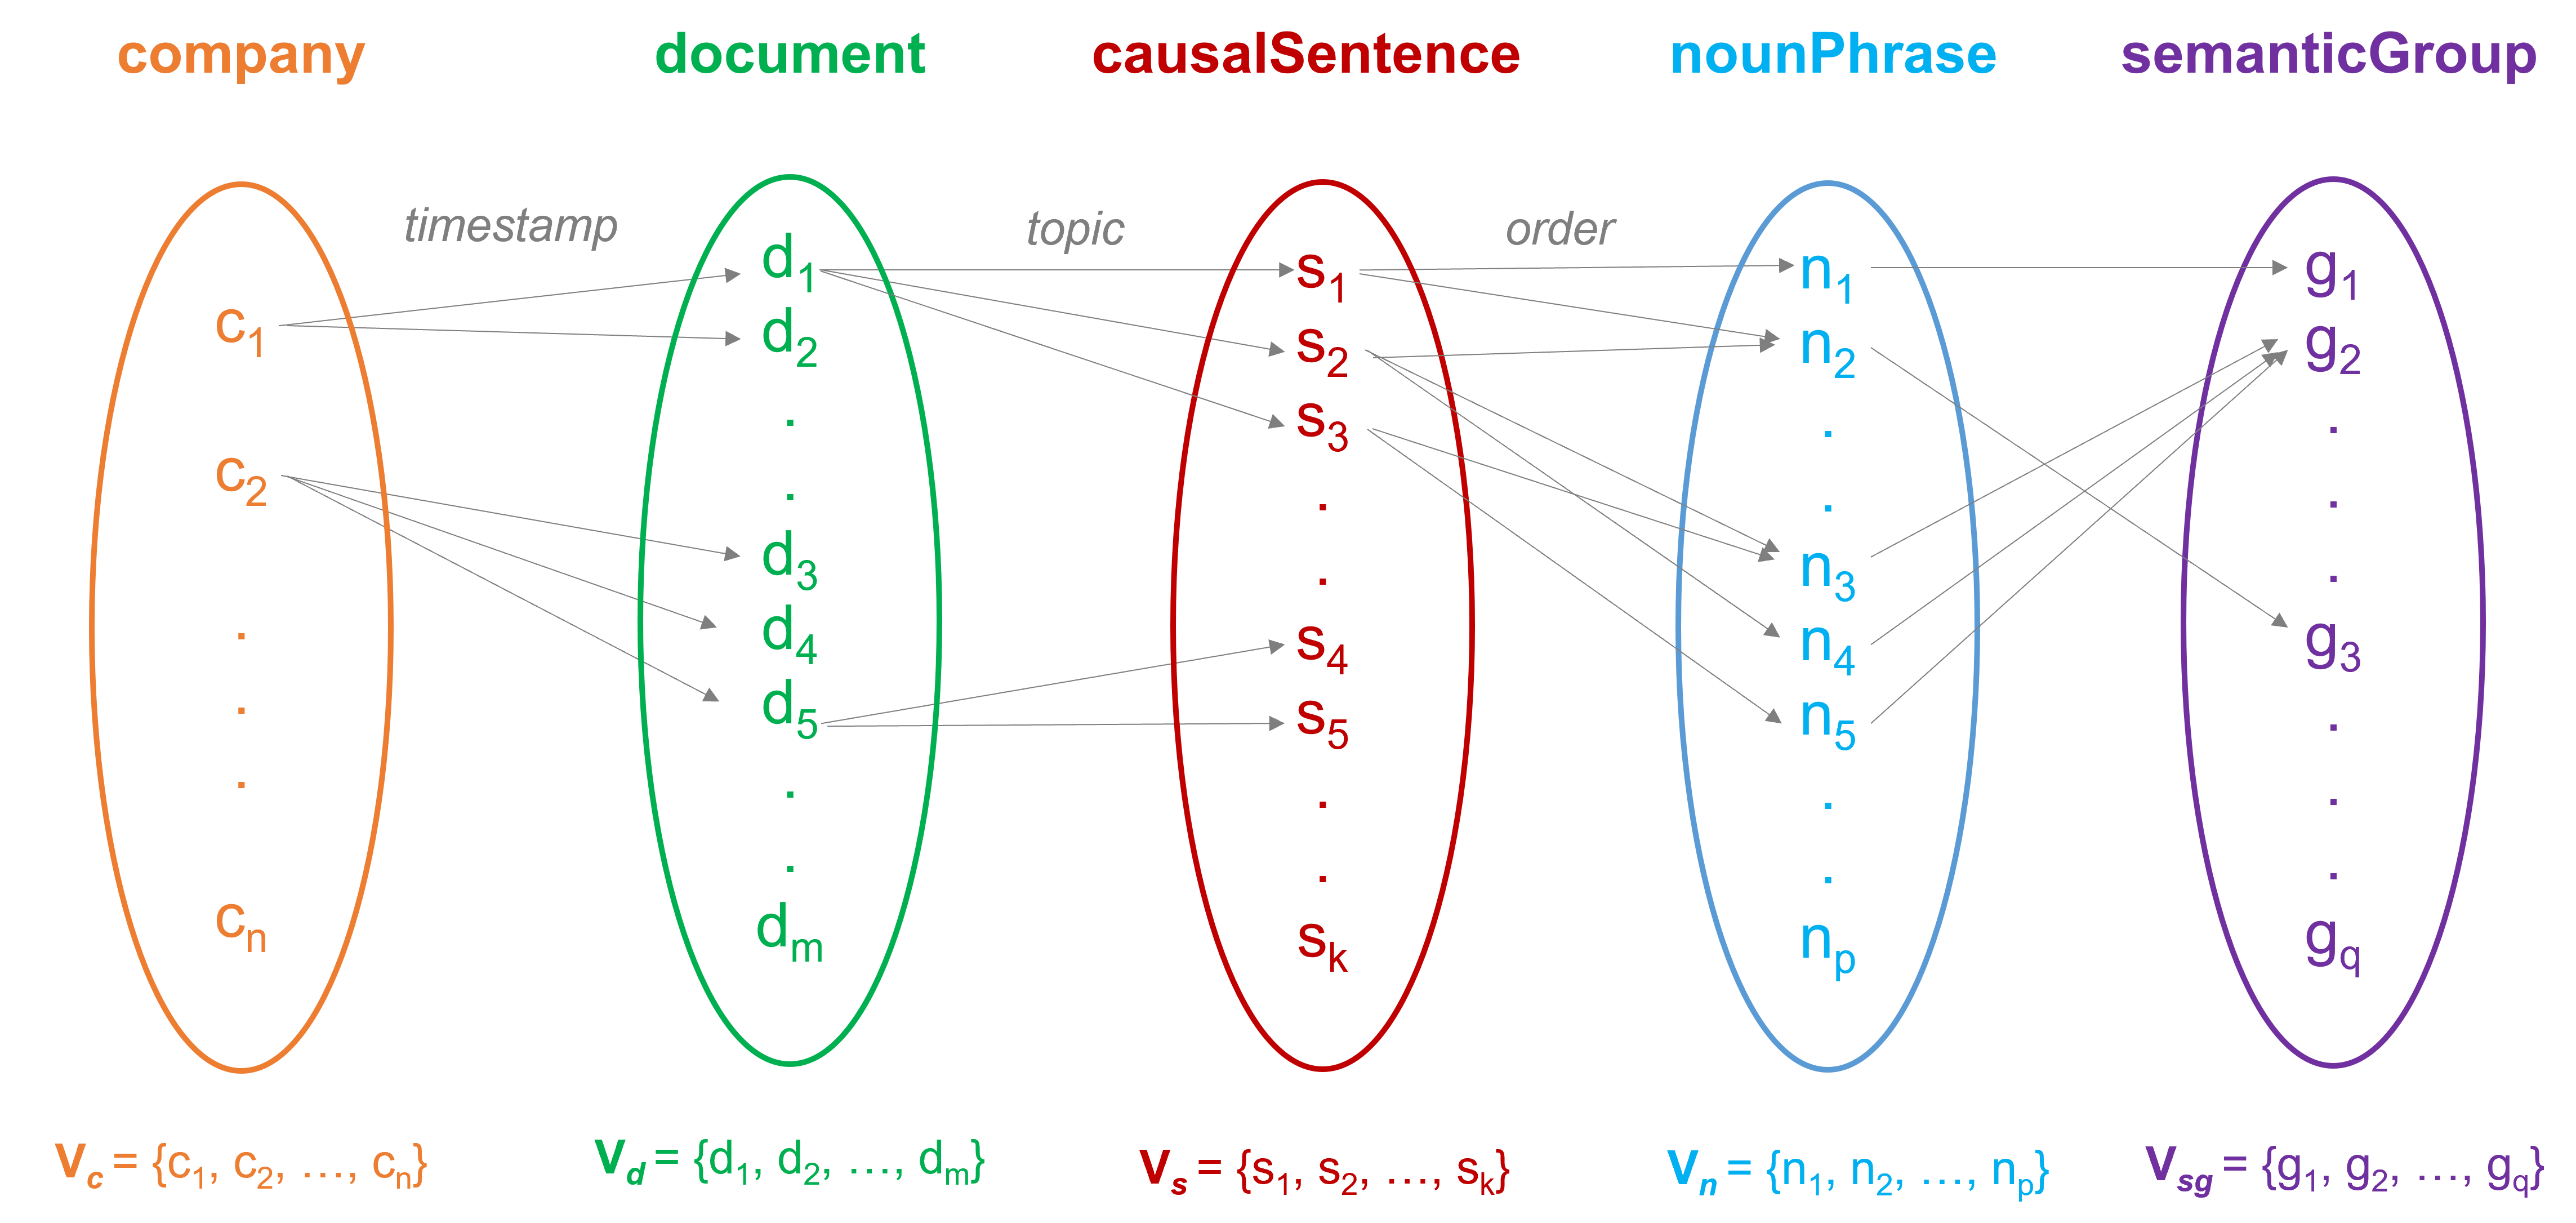
\includegraphics[scale=0.4]{figures/Sets.png}
  \caption{Illustration of set relationships among the company set, document set, causalSentence set, nounPhrase set and concept set.}
  \label{fig:AssumpSet}
\end{figure}

The primary goal of breaking the causal clauses into noun phrases is to transform the data model into a high dimensional latent space, where each specific cause is decomposed into individual features or latent factors. The primary goal of clustering noun phrases into concepts is to detect the hidden patterns and reduce the dimensionality of the sparse latent space. This effectively achieves data compression for generalization and data association in order to facilitate data retrieval. In addition, these concept clusters also enable direct connections to be made between companies which might be affected by implicitly similar factors that are semantically close in the latent space, but not expressed by exactly the same causal clauses at the explicit level. 

In summary, our data model has the following characteristics: 

\begin{itemize}
	\item	 It is a heterogeneous graph with five distinct types of nodes: \emph{Company, Document, CausalSentence, NounPhrase, and ConceptCluster}.
	\item	 These nodes follow a natural hierarchical order: \emph{Company $\rightarrow$ Document $\rightarrow$  CausalSentence $\rightarrow$ NounPhrase $\rightarrow$ ConceptCluster} 
	\item 	Concept nodes can be perceived as the connection points providing the means for similarity measures at different node levels. 
	\item 	Temporal information included in the graph make it possible to treat it as a dynamic graph, where an evolution of trends can be observed with respect to the passage of time. 
	\item 	The data model can be incrementally updated, when new financial reports become available.
\end{itemize}




%%%

\subsection{Node Embeddings and Similarity Measures} \label{sec:similarity}

Having established the basics of the data model, we now move on to define node embeddings and similarity measures between nodes. This paves the foundation for directly addressing the two objectives stated earlier in Section 3.1: the identification of performance drivers and the discovery of similar companies. Node embeddings and similarity measures are defined according to their respective node types.


% NounPhrase
\paragraph{NounPhrase Node Embedding:} Since a $NounPhrase$ node represents a noun or a noun phrase, the underlying word embedding is a natural choice for the node embedding. Different types of word embeddings, such as word2vec, GloVe and BERT, have already been discussed in Section 2.2.1. In addition, the various methods for computing phrase represenations from word vectors have also been discussed in Section 2.2.2. A suitable choice for the noun phrase node embeddings in our data model is a static word-level embedding model pre-trained on a relatively large corpora, such as pretrained GloVe embeddings. A simple average operation is opted for obtaining the compositional phrase embeddings from the constituents word embeddings. 
\[ \mathbf{Embedding}(NounPhrase) = \frac{1}{n} \sum_{i=1} ^n {\mathbf{w_i}}\]  
where $\mathbf{w_i}$ is the word embedding for the $i^{th}$ token in the $NounPhrase$ and $n$ is the total number of tokens in the $NounPhrase$. 

The similarity between a pair of $NounPhrase$ nodes is defined as the cosine similarity between the node embeddings. 
\[ \mathbf{Similarity}(NounPhrase_A, NounPhrase_B) = \frac{\mathbf{A \cdot B} } {\mathbf{\lVert A \rVert \cdot \lVert B \rVert}} \]  where $\mathbf{A}$ = \textbf{Embedding}($NounPhrase_A$), $\mathbf{B}$ = \textbf{Embedding}($NounPhrase_B$).

These similarity measures allows the grouping together of noun phrases which are closely related in semantics, while spacing wider apart the ones which are distantly related. These node embeddings are used as input to the clustering algorithm which generate $Concept$ nodes.

% Concept
\paragraph{Concept Node Embedding:} A $Concept$ node is effectively the centroid of the clusters of $NounPhrase$ nodes which are directly connected to it in the graph. The node embedding for a $Concept$ node is defined as:
\[ \mathbf{Embedding}(Concept) = \frac{1}{m} \sum_{j=1} ^n {\mathbf{V_j}}\] 
where $\mathbf{V_j}$ is the node embedding for the $j^{th}$ $NounPhrase$ in the immediate neighborhood of the $Concept$ node and $m$ is the total number of $NounPhrase$ nodes in the neighbourhood. 

The similarity between a pair of $Concept$ nodes is defined as the cosine similarity between the node embeddings. 
\[ \mathbf{Similarity}(Concept_X, Concept_Y) = \frac{\mathbf{X \cdot Y} } {\mathbf{\lVert X \rVert \cdot \lVert Y \rVert}} \]  where $\mathbf{X}$ = \textbf{Embedding}($Concept_X$), $\mathbf{Y}$ = \textbf{Embedding}($Concept_Y$).


% CasualSentence
\paragraph{CausalSentence Node Embedding:} Each $CausalSentence$ node is connected to an ordered set of $NounPhrase$ nodes that represent the constituent underlying noun phrases according to their order of appearance in the cause chunk of the sentence. Each $NounPhrase$ node is in turn connected to a $Concept$ node. Therefore, the node embedding for a $CausalSentence$ node can be represented as a list of $Concept$ node indices: 
\[ \mathbf{Embedding}(CausalSentence) = [cc_1, cc_2, ..., cc_i, ..., cc_n] \]
where $cc_i$ is the index of the $Concept$ node linked to the $NounPhrase$ node, which is connected to the $CausalSentence$ node with an edge order = $i$; $n$ is the total number of $NounPhrase$ nodes connected to the $CausalSentence$ node. 

The $CausalSentence$ node embeddings are allowed to have different lengths according to how many $NounPhrase$ nodes there are in its neighborhood. In other words, the lengths of the node embeddings also encode the amount of information content in the sentences represented by the $CausalSentence$ nodes. 

The similarity between a pair of $CausalSentence$ nodes is measured at two levels: weak similarity and strong similarity. The weak similarity is defined as the Jaccard similarity between the two node embeddings of the $CausalSentence$ nodes:
\[ \mathbf{Similarity}(CausalSentence_A, CausalSentence_B) = \frac{\| \mathbf{A \cap B} \|}{\|\mathbf{A \cup B} \|} \]  
where $\mathbf{A}$ = \textbf{Embedding}($CausalSentence_A$), $\mathbf{B}$ = \textbf{Embedding}($CausalSentence_B$).

Only if the weak similarity between two $CausalSentence$ nodes are above a certain threshold, then the strong similarity is defined. The strong similarity is used as a more precise measure of how similar the pair of nodes are when they are already considered somewhat similar by the weak similarity measure. If the pair of nodes has a weak similarity below the threshold, for example, when the pair of $CausalSentence$ nodes do not share any $Concept$ nodes in common, there is no practical need to further compute the strong similarity score between them. 

There are various methods to define the strong similarity, such as Levenshtein distance \cite{similarity2020} or Sorenseon-Dice coefficient \cite{similarity2020} based on the $CausalSentence$ node embeddings; alternatively, a cosine similarity between the sentence embeddings of the underlying text can be obtained from a pretrained model such as Sentence-BERT \cite{sentenceBERT2019}. The precision required for the strong similarity measure depends on the end application and how much computational resources are available in practice. The exploration in this regard is left to future studies. 

For the purpose of this thesis, only the weak similarity measure is applied, as there is no practical need to compare two individual sentences in the end application. 


% Document
\paragraph{Document Node Embedding:} Each $Document$ node is connected to a set of $CausalSentence$ nodes via edges labelled with $topics$, which are financial KPIs explained by the causal sentences. Accordingly, the $Document$ node embedding is defined as the collection of different sets of the $CausalSentence$ node embeddings, where $CausalSentence$ notes in each set correspond to a distinct $topic$. 
\[ \mathbf{Embedding}(Document) =  \{ \mathbf{D_t} \mid t \in topics(Document) \} \]
where
\[ \mathbf{D_t} = \{ \mathbf{Embedding}(CausalSentence_i) \mid CausalSentence_i \in \mathcal{N}_t(Document) \} \]
and $\mathbf{D_t}$ represents a set of $CausalSentence$ node embeddings under a topic $t$, $topics(Document)$ represents the set of $topics$ on the outgoing edges of the $Document$ node, $\mathcal{N}_t(Document)$ represents the set of $CausalSentence_i$ nodes in the immediate neighborhood of the $Document$ node under the topic $t$.

Equivalently, each $Document$ node embedding can be expressed in the form of a matrix, where each column is a vector representation of the distribution of the $Concept$ nodes under a $topic$. The dimension of the column vector is equal to the total number of unique $Concept$ nodes and each entry in the embedding corresponds to the number of counts for each $Concept$ node.
\[ \mathbf{Embedding}(Document) =  (d_{i,j}) \in \mathbb{R}^{m \times n} \] 
where $m=\mid \mathbf{V}_{Concept} \mid$,  $n=\mid \mathbf{E}_2 \mid$.

The similarity measure between two $Document$ nodes is defined as the cosine similarities of each pair of corresponding column vectors of the two nodes embedding matrices. The resulting representation is a row vector with each entry representing the similarity measure for each topic.
\[ \mathbf{Similarity}(Document_A, Document_B) = [ \mathbf{s_j} ] \in \mathbb{R}^{1 \times n}\]
\[  \mathbf{s_j} = \frac{\mathbf{a_j \cdot b_j} } {\mathbf{\lVert a_j \rVert \cdot \lVert b_j \rVert}} \]  
where 
\[ \mathbf{a_j} = \textbf{Embedding}(Document_A)[: , j] \]
and 
\[ \mathbf{b_j} = \textbf{Embedding}(Document_B)[: , j] \]


% Company
\paragraph{Company Node Embedding:} Each $Company$ node is connected to a set of $Document$ nodes through timestamped edges. A $Company$ node embedding is therefore represented as a tensor, i.e., a stack of $Document$ embedding matrices each representing a discrete timestamp. This approach naturally supports generating dynamic $Company$ node embeddings based on the specification of $time periods$ according to the use cases. 
\[ \mathbf{Embedding}(Company_{t_1}^{t_2}) = \sum_{t=t_1} ^{t=t_2} {\mathbf{Embedding}(Document_t)}\]  
where $Document_t \in \mathcal{N}_t(Company)$, the neighborhood of the $Company$ node for the specified period from $t=t_1$ to $t=t_2$. 

For a specified time period, the three-dimensional tensor representations of a $Company$ node embedding can be effectively transformed into a two-dimensional matrix by aggregating along the temporal axis by summation; the resulting matrix representation is effectively in the same form as a $Document$ node embedding as described above. 

The similarity measure between two $Company$ nodes, $(Company_A)_{t_1}^{t_2}$ for the time period from $t1$ to $t2$ and $(Company_B)_{\tau_1}^{\tau_2}$ for the time period from ${\tau_1}$ to ${\tau_2}$, are defined the cosine similarities of each pair of corresponding column vectors of the two nodes embedding matrices:
\[ \mathbf{Similarity}((Company_A)_{t_1}^{t_2}, (Company_B)_{\tau_1}^{\tau_2}) = [ \mathbf{s_j} ] \in \mathbb{R}^{1 \times n}\]
\[  \mathbf{s_j} = \frac{\mathbf{a_j^{T} \cdot b_j^{\mathcal{T}}} } {\mathbf{\lVert a_j^{T} \rVert \cdot \lVert b_j^{\mathcal{T}} \rVert}} \] 
where 
\[\mathbf{a_j^{T}} = \textbf{Embedding}((Company_A)_{t_1}^{t_2})[: , j] \] 
and
\[\mathbf{b_j^{\mathcal{T}}} = \textbf{Embedding}((Company_B)_{\tau_1}^{\tau_2})[: , j] \]

This approach not only allows the optional tracking of the temporal evolution of the $Company$ node embeddings at various granularity levels, e.g., quarterly, annually or every five years, but also enables comparison of companies across different periods of time. 


\newpage

%%%%%%%%%%%%%%%%%%%%%%%%%%%%%%%%%%%%%%%%%%%%%%%%%%%%%%%%%%%%

\chapter {Implementation and Experimental Results} \label{implementation}

%\chapter {Implementation and Experimental Results} \label{implementation}

[Add intro...]
The structure of this chapter or its division into two chapters
heavily on the subject and the treatment of the subject
dependent. Data are described here that are required for an evaluation
is used (sources, examples, statistics), the objective of the evaluation
and the measures used as well as the results (e.g.~with the help of
charts, diagrams, illustrations, etc.)

This chapter can also include a description of the realization of a
systems (no source code, maximum class diagrams!).

\section {Data Collection} 

\subsection {Download from EDGAR}

Our dataset consists of the quarterly and annual financial reports from S\&P 500 companies. More specifically, electronic filings of form 10-Q and form 10-K for each of the publicly listed companies are downloaded from the SEC EDGAR site (see Section \ref{subsec:SEC}). With the aid of the Python library, \emph{sec-edgar-downloader}\footnote{ https://sec-edgar-downloader.readthedocs.io }, a total of 40,628 files covering a period of 20 years from 2001 to 2021 has been downloaded. The total size of the files sums to exceed 85 GB and it takes ca. 17 hours to complete the download. Figure \ref{fig:byYear}  shows the distribution of the number of files by year and Figure \ref{fig:byIndustry} shows the distribution of the number of companies by industry. 

These files are encoded in a variety of formats: those filed in early 2000s are generally in TXT, PDF or PowerPoint format, and the more recent filings are in HTML format. This is mainly due to the historical changes in SEC standards and the different time frames of adoption by different companies  (see Section \ref{subsec:SEC}).
 
Furthermore, each document in the dataset has certain metadata associated with it, such as the company ticker, company name, file type, file name and published year. Figure \ref{fig:meta} shows a few examples in the meta datasheet. This information is used to populate the data model described in Chapter \ref{conceptualization}. 

\begin{figure}[!tbp]
  \centering
  \begin{minipage}[b]{0.45\textwidth}
    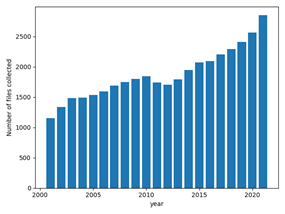
\includegraphics[width=\textwidth]{figures/byYear.png}
    \caption{Distribution of the number of files by year}
    \label{fig:byYear}

  \end{minipage}
  \hfill
  \begin{minipage}[b]{0.45\textwidth}
    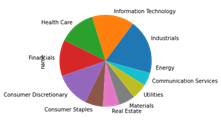
\includegraphics[width=\textwidth]{figures/byIndustry.png}
    \caption{Distribution of the number of companies by industry}
    \label{fig:byIndustry}

  \end{minipage}
\end{figure}


\begin{figure}[h!]
\centering
  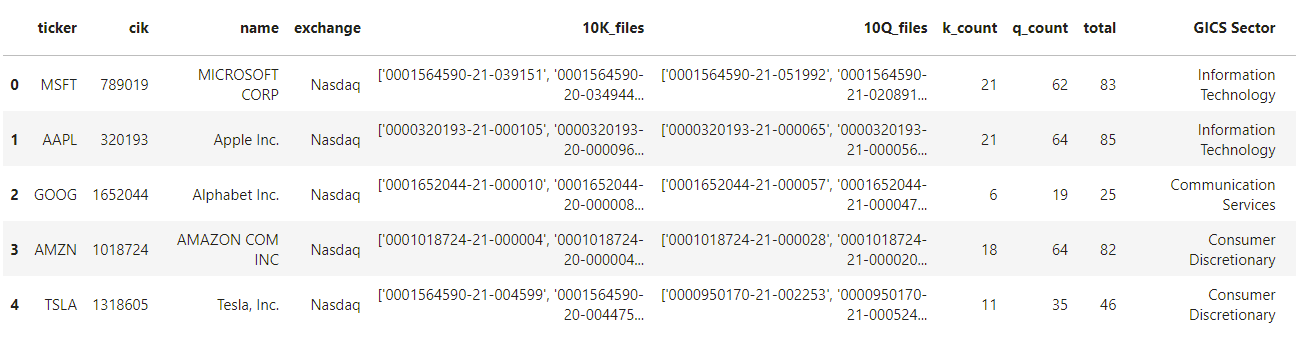
\includegraphics [width=\textwidth]{figures/meta.png}
  \caption{Snapshot of the Meta Information Sheet}
  \label{fig:meta}
\end{figure}



\subsection {Identity MD\&A Sections}

Due to the sheer size of the dataset and potentially formidable computational cost associated with the subsequent storage and search operations, it is necessary as a first step to filter the dataset in order to focus only on the most relevant information. In this case, we have already identified MD\&A section in these financial reports as the most relevant. Hence, the first step in our pipeline is to preprocess the raw data to extract the MD\&A section. 

To start, \emph{BeautifulSoup}\footnote{https://beautiful-soup-4.readthedocs.io} is employed to parse HTML files into raw texts. Then our system uses manually constructed rules to detect the start and end positions of the MD\&A section based on regular expressions. For 10-Qs, the MD\&A sections are typically found under the heading 'Part I.  Item 2' and for 10-Ks, the MD\&A sections are found under the heading 'Part II. Item 7'. After identification of the start and end position of a MD\&A section, the   

A total of 32,807 MD\&A sections (ca. 81\% of all files downloaded) are successfully extracted after the preprocessing step. There are 7,821 files that are disregarded by our system, because they do not contain a valid MD\&A section or our system could not identify either the start or the end position in the raw text file. Figure \ref{fig:MDAidentified} shows success rate of MD\&A extraction from raw files across all years. The earlier years have a much lower identification rates, as the early filings are not as standardized as compared to filings in recent years due to the tightening of the regulation requirements as already discussed in Section \ref{subsec:SEC}.

Figure \ref{fig:MDAlen} shows the distribution of length of the MD\&A sections by number of characters. The average length of MDA is ca. 70,217 characters. As an initial exploration, we extract the most frequent words by part-of-speech. Figure \ref{fig:NOUN} and Figure \ref{fig:VERB} in Appendix \ref{appendix:EDA} illustrate the top 100 nouns and verbs, respectively, from these MD\&A sections. The exploratory data analysis reveals some key characteristic of the MD\&A sections that the vocabulary is domain-specific and there seems to be certain patterns of language used in these texts.

\begin{figure}[!tbp]
  \centering
  \begin{minipage}[b]{0.45\textwidth}
    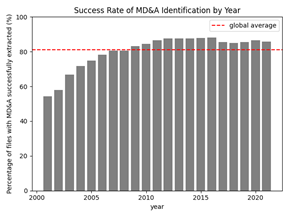
\includegraphics[width=\textwidth]{figures/MDAidentified.png}
    \caption{Success rate of MD\&A identification from raw files by by year}
    \label{fig:MDAidentified}

  \end{minipage}
  \hfill
  \begin{minipage}[b]{0.45\textwidth}
    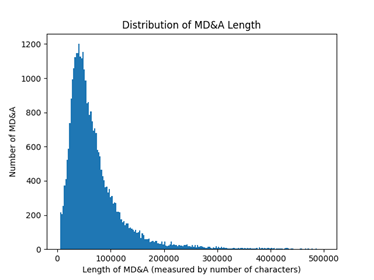
\includegraphics[width=\textwidth]{figures/MDAlen.png}
    \caption{Distribution of MD\&A lengths by number of characters}
    \label{fig:MDAlen}

  \end{minipage}
\end{figure}



\section{System Implementation} 
This section describes the implementation details of the pipeline. As illustrated in Figure \ref{fig:pipeline}, the input to the system consists of raw texts from the MD\&A sections. There are two main modules in the pipeline: Extraction and Clustering. The output of the system is the data model as described in Chapter 3. The pipeline is implemented in Python with external open-source libraries such as \emph{spaCy}\footnote{https://spacy.io/} for text processing and \emph{neo4j}\footnote{https://neo4j.com/product/neo4j-graph-database/} as the graph database for our data model. 

\begin{figure}[h!]
\centering
  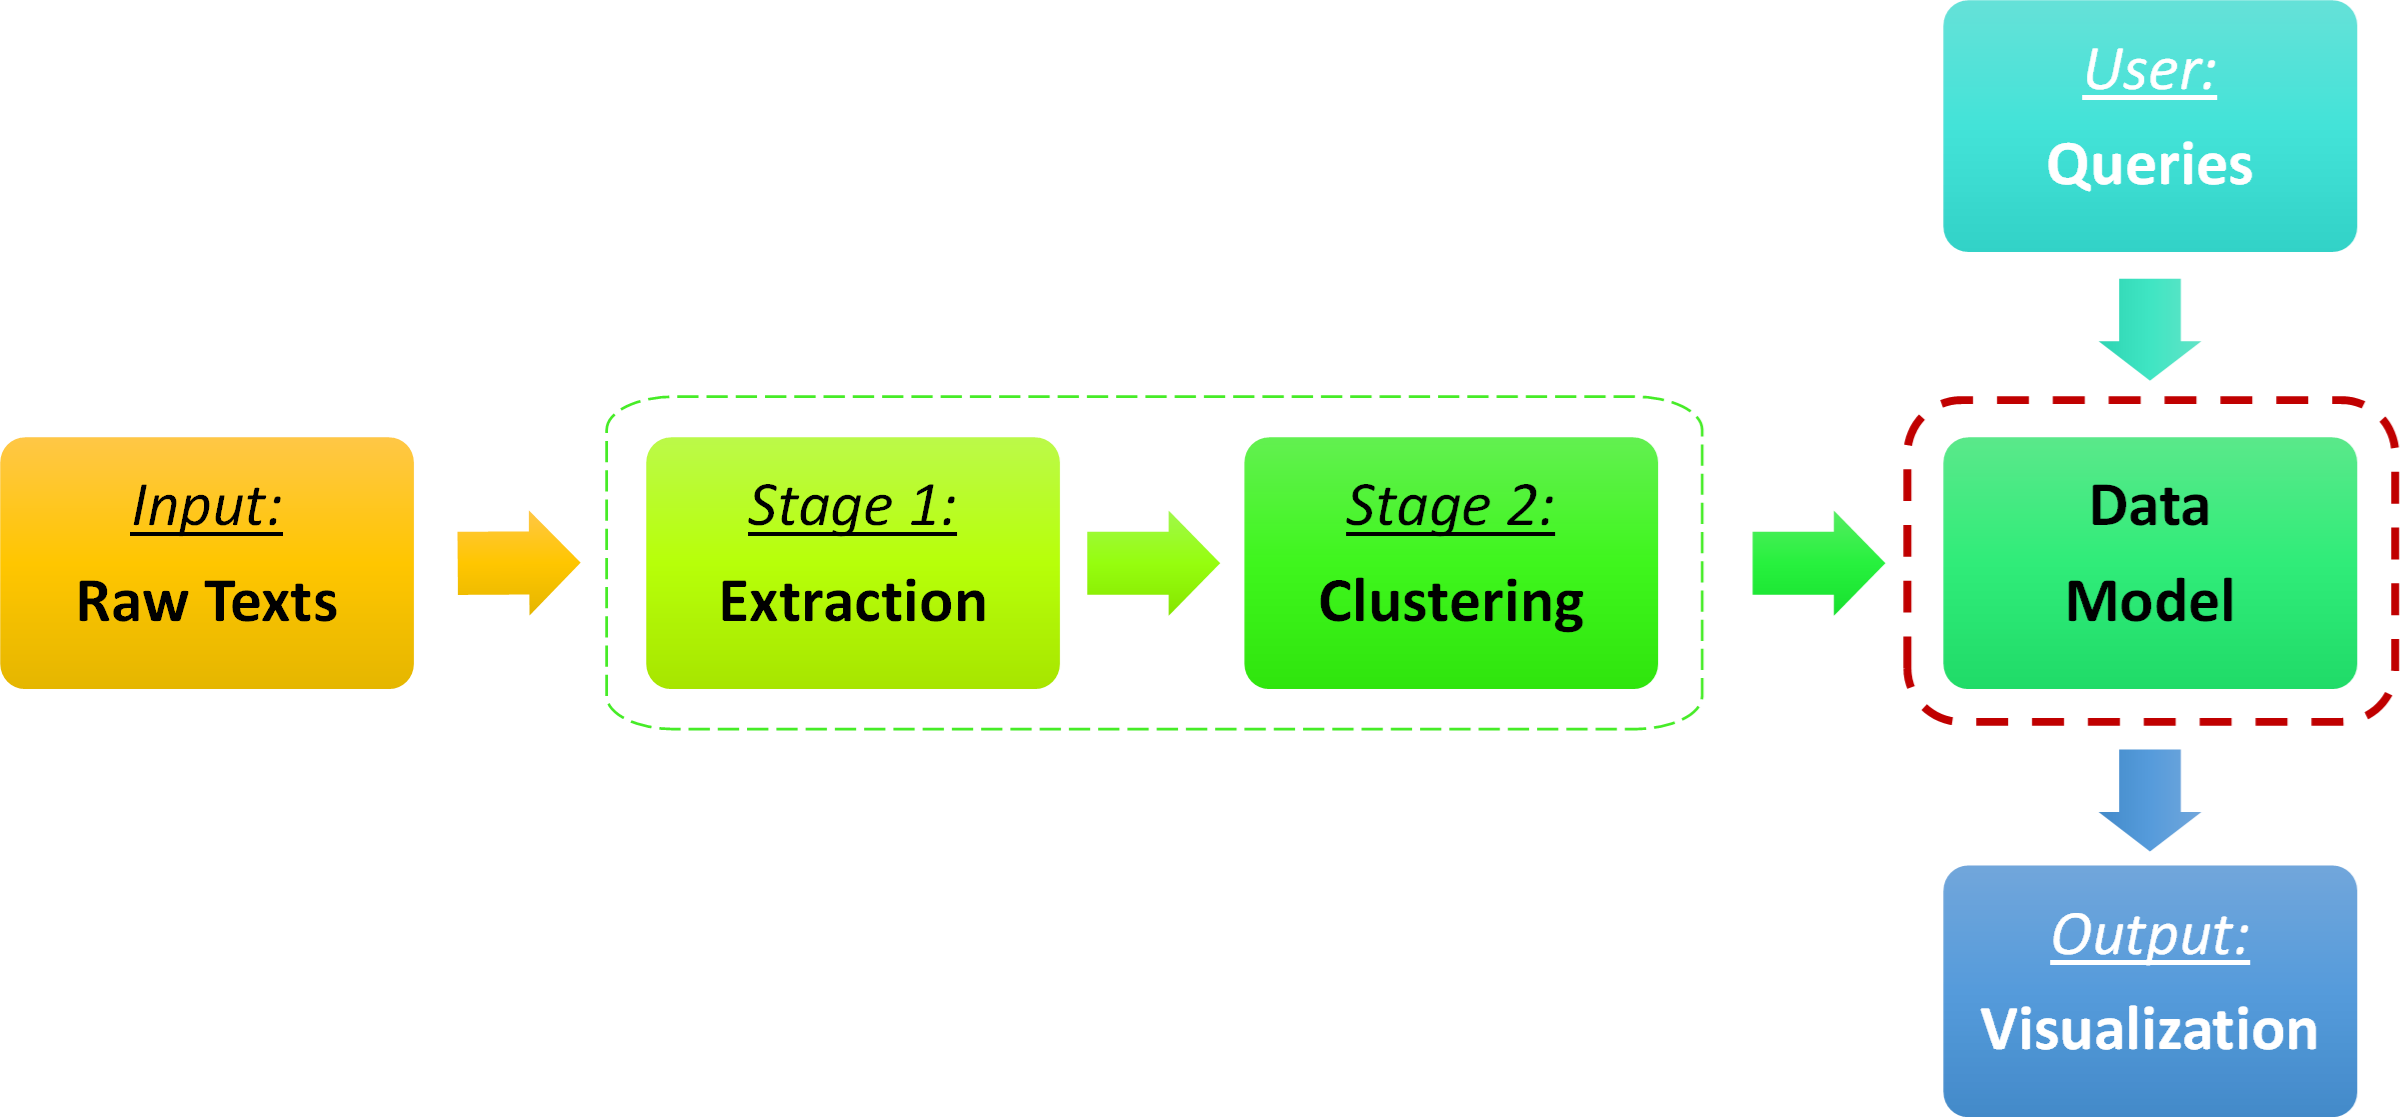
\includegraphics[scale=1.4]{figures/Pipeline_0.png}
  \caption{Illustration of Data Processing Pipeline}
  \label{fig:pipeline}
\end{figure}


\subsection{Extraction}
The extraction module identifies causal sentences and extracts causal factors in the form of noun phrases from these causal sentences. 

When a raw MD\&A text file is input into our pipeline, it is first split into sentences. Sentences that are too short (less than 50 characters), too long (more than 500 characters) or without any verb in the predicate, are discarded. The purpose of this preprocessing step is to filter off headings, section titles, bullet points, financial tables, and other text fragments, so that only proper, complete sentences are processed in this module.

As discussed in Section 3.3, only sentences containing causal explanations are regarded as relevant to our system's downstream processing. To extract these causal sentences, our system implements a linguistic pattern-based framework. The most commonly used causal markers from the MD\&A sections are manually identified. The current list includes the following causal connectives: 

\begin{itemize}
\item	verbs: \emph{result, affect, impact, cause, contribute, attribute, drive, relate, associate, reflect}
\item	non-verbs: \emph{due to, because, attributable to, as a result of, in connection with}
\end{itemize}

After the preprocessing step, each sentence is checked for the presence of causal connectives specified in the two lists above. For the sentences classified as causal, the system further process them to extract the cause and effect chunks. For example, in the sentence \emph{"For the quarter ended June 30, 2020, our advertising revenues declined due to the continued impacts of COVID-19 and the related reductions in global economic activity"}, the causal connective, \emph{"due to"}, qualifies the sentence as as a causal sentence. Accordingly, the template "\textbf{[effect chunk]} \emph{due to} \textbf{[cause chunk]}" is evoked. The sentence is parsed into the cause chunk, i.e., \emph{"the continued impacts of COVID-19 and the related reductions in global economic activity"} and the effective chunk, i.e., \emph{"For the quarter ended June 30, 2020, our advertising revenues"}, respectively. 

The system further extracts useful information from the cause and effect chunks. A topic of interest, e.g., \emph{"revenue"}, is identified from the effect chunk in the example sentence above. In addition,  noun phrases are extracted from the cause chunk with the help of SpaCy's default dependency parser, where noun phrases are defined as the \emph{"flat phrases that have a noun as their head"}\footnote{ https://spacy.io/usage/linguistic-features\#noun-chunks}. In laymen's term, it means that a noun plus the words describing the noun. In the example sentence quoted above, \emph{"The continued impacts", "the related reductions"} and \emph{"global economic activity"} are the noun phrases extracted from the cause chunk. 

Figure \ref{fig:chunks} provides a graphical illustration of the various parts of the example sentence identified by the extraction module. A total of 1,003,152 causal sentences are collected with a pre-defined list of topics, including the following terms: \emph{revenue, sale, cost, expense, margin, profit, earning, income,} and \emph{loss}. These causal sentences have an average length of 246 characters. From these causal sentence, a total of 5,069,900 noun phrases are extracted, of which 455,538 are unique. These unique noun phrases are to fed into the clustering module at the next stage of the pipeline for further processing.  

\begin{figure}[h!]
\centering
  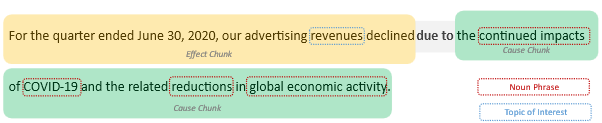
\includegraphics[width=\textwidth]{figures/CEchunks.png}
  \caption{Illustration of an example causal sentence and its cause and effect chunks with the identified topics of interest as well as noun phrases}
  \label{fig:chunks}
\end{figure}


The primary reasons for choosing a simple linguistic pattern-based system for causality extraction over the state-of-the-art deep neural models are three-fold. Firstly, training a deep neural model such as Bi-LSTM \cite{Li21BiLSTMCRF,Chen20} or BERT-CRF \cite {NTUNLPL20}, requires an annotated dataset of a reasonably large size, which we do not have. To commission such an annotation task based on our dataset is not only time-consuming but also costly. To leverage the existing datasets such as FinCaual \cite{FinCausal20} and SemEval \cite{SemEval07Task4, SemEval10Task8} is also not a viable option, because the tagging schemes are conceivably different from what this pipeline requires. 

Secondly, we recognize that interpretability and explainability are both very important for financial decision-making. Deep neural networks are black-box solutions inherently lacking interpretability. Their improved predictive accuracy has often been achieved through increased model complexity \cite{explainableAI2021}. In contrast, a rule-based system gives users the complete control over the causal sentence specification. It is not only transparent and accountable, but also computationally more efficient than deep neural models.  

Last but not least, we know from experience that the language style and sentence structures in these financial reports tend to conform to certain patterns, which can be exploited using rule-based heuristics. Our system may not generalize well in a domain agnostic scenario, however, it performs at a reasonable level of satisfaction for the domain-specific causal sentence extraction task at hand (see evaluation results in Section \ref{sec:evaluate}. In essence, our system is built based on the practicality of solving a problem using a minimal and frugal design.


\subsection{Clustering}
The clustering module of the pipeline processes the unique noun phrases collected from the preceding extraction module and group them into clusters according to their semantic similarity. These noun phrase clusters are referred to as concept clusters, as defined in Section 3.3.

For pretrained word embedding, our system uses the 'glove-wiki-gigaword-50' model \cite{glove2014}, downloaded from the Gensim-data repository\footnote{https://github.com/RaRe-Technologies/gensim-data}. The model has been trained on a combination of the Wikipedia 2014 dump and the Gigaword 5 corpus, with six billion uncased tokens, of which 400,000 are unique tokens\footnote{https://nlp.stanford.edu/projects/glove/}. Each word vector has 50 dimensions. To represent a noun phrase, our system takes the simple average of all word embeddings in the noun phrase and normalizes to a range of [-1,1] before feeding into the clustering algorithm.

For clustering, our system implements the SOM algorithm using the miniSOM library\footnote{ https://pypi.org/project/MiniSom/}. The number of neurons is decided based on the rule of the thumb \cite{SOM2019, SOM2014} that the total number of neurons should be $5\times \sqrt{N}$ where $N$ is the number of data points in the training set. In our case, $N = 455,539$, which is the number of unique noun phrases. Accordingly, a SOM with $3,364$ neurons arranged in a grid size of $58 \times 58$ is chosen. This particular topology is also chosen for the convenience of facilitating the final data visualization on a 2D map.

The network of the neurons are initialized with random weights and the neighborhood function is set to Gaussian. The optimal sigma and learning rate are determined through experimentation. The quantization error and topographic error (see Section 2.2.3) are used as the evaluation metrics for the SOM model performance. As illustrated in Figure \ref{fig:sig} and \ref{fig:lr}, we choose sigma = 2.5 and learning rate = 0.25 for our model. Furthermore, as illustrated in Figure \ref{fig:epoch}, we find that increasing the number of epochs (i.e. number of times that the SOM is trained on the entire dataset) does not affect the quantization error and the topographic error after the first pass. 

\begin{figure}
     \centering
     \begin{subfigure}[b]{0.3\textwidth}
         \centering
         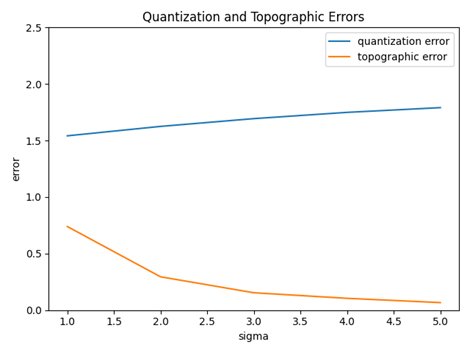
\includegraphics[width=\textwidth]{figures/SOM_sigmas.png}
         \caption{Sigma}
         \label{fig:sig}
     \end{subfigure}
     \hfill
     \begin{subfigure}[b]{0.3\textwidth}
         \centering
         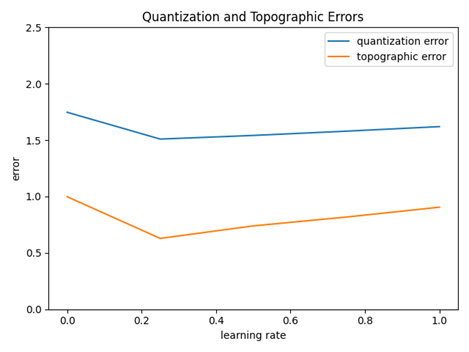
\includegraphics[width=\textwidth]{figures/SOM_learningrates.png}
         \caption{Learning Rate}
         \label{fig:lr}
     \end{subfigure}
     \hfill
     \begin{subfigure}[b]{0.3\textwidth}
         \centering
         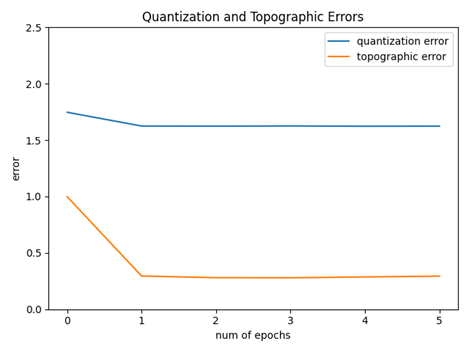
\includegraphics[width=\textwidth]{figures/SOM_epochs.png}
         \caption{Epoch}
         \label{fig:epoch}
     \end{subfigure}
        \caption{Quantization and Topographic Errors}
        \label{fig:experiments}
\end{figure}


Figure \ref{fig:distanceMap} shows the distance map of neuron weights of the SOM after training is complete. The color of each cell corresponds to the normalized sum of the Euclidean distances of that underlying neuron's weight to all its neighboring neurons'. It is effectively a visualization of how similar each neuron is to its neighbors and provides some indication for merging similar neurons into a larger clusters, i.e., the lighter regions on the map separated by darker boundaries.  

Figure \ref{fig:activationMap} shows the activation map of the SOM after training. The activation map is a matrix representation of the neurons network where the color intensity corresponds to the number of times that underlying neuron have been the winner during the competitive learning (see Chapter 2). In another words, the darker the cell is, the more data points has it seen during the training which have updated its weight. Therefore, it is also an indication of how many data points are associated with the underlying neuron.  


\begin{figure}
     \centering
     \begin{subfigure}[b]{0.45\textwidth}
         \centering
         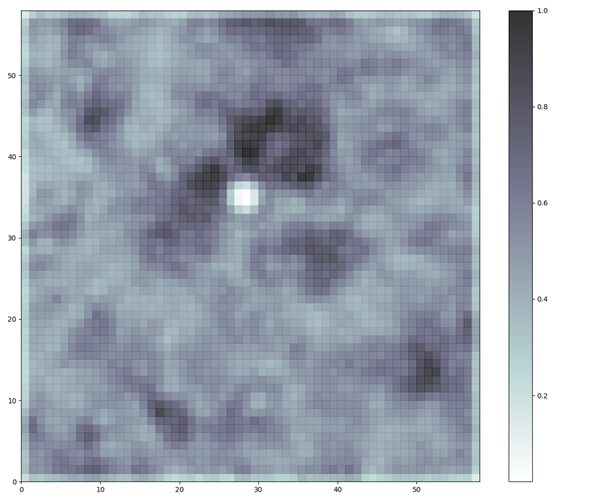
\includegraphics[width=\textwidth]{figures/SOM_distance.png}
         \caption{Distance Map}
         \label{fig:distanceMap}
     \end{subfigure}
     \hfill
     \begin{subfigure}[b]{0.45\textwidth}
         \centering
         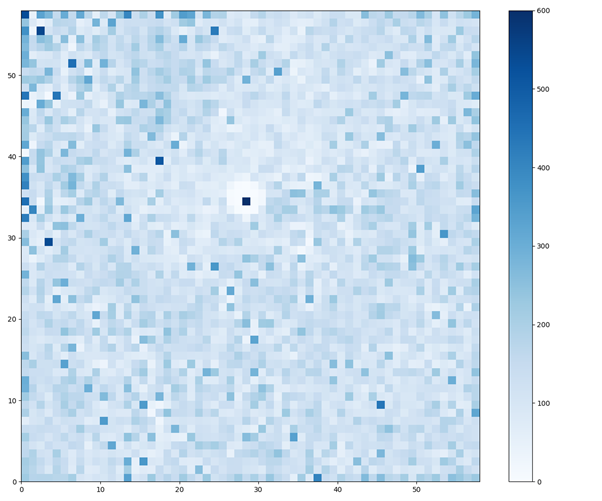
\includegraphics[width=\textwidth]{figures/SOM_activation.png}
         \caption{Activation Map}
         \label{fig:activationMap}
     \end{subfigure}
        \caption{2D map representations of the SOM after training. Distance Map is a visualization of how similar each neuron is to its neighbors. The Activation Map is a matrix representation of the neurons network where the color intensity corresponds to the number of times that underlying neuron have been the winner.}

\end{figure}

For the clustering module in our system, we choose SOM instead of K-means, as we do not know the optimal number of clusters, which is required as a hyper-parameters in the latter. In theory, we could use the Elbow's method \cite{elbow2020} to determine the optimal number of clusters, however, it does not provide a direct visual output illustrating the distances between the clusters. Some post-processing is needed in order to represent the clusters in a 2D map as the SOM output. 

Furthermore, due to the size of the dataset ($N=455,538$), hierarchical clustering is not suitable in terms of computation time and memory space required. The space complexity for hierarchical clustering is $O(N^2)$ with the storage of the similarity matrix in the RAM. In addition, the most naive implementation of the hierarchical clustering has a time complexity of $O(N^2 log N)$ \cite{clustering1999}. In contrast, both the SOM and the k-means algorithm have a linear time complexity of $O(NM)$, where M is the number of pre-specified clusters in K-means and the number of neurons in SOM, respectively. In terms of space complexity, K-means has $O(N+M)$ \cite{clustering1999} and SOM has $O(M^2)$ \cite{complexity2017}.  

[TODO: perform hierarchical clustering on the SOM output to reduce the number of clusters.] 

[TODO: to repeat the experiments with W2V 300 embeddings and check the quality of clustering]


\subsection{Data Model Implementation}

To implement the data model, we use Neo4j Community Edition 4.0.4 \footnote {https://neo4j.com/}, which is designed to handle graph data natively. We create different types of nodes and the corresponding edges according to the data model described in Chapter 3. 
More specifically, company nodes are created with the following properties: \emph{ticker, company name, sector classification}. Document nodes are created only for those that the MD\&A sections are identified. The document nodes have properties such as \emph{ticker, file name, file type (10-K or 10-Q)}. Edges are established between the company nodes and the document nodes where they share the same tickers. The edges are labeled with a property that specified the year of the document's publication.

For causal sentences identified by the causality extraction module of our system, causal sentence nodes are created with the following properties: \emph{raw text of the causal sentence, previous sentence, next sentence} (to provide some context). Edges are established between each causal sentence and the document it belongs to with a property that is labeled as \emph{topic}.

Noun phrase nodes are created for all the noun phrases extracted from the cause chunks of the causal sentences. Each node has the raw text of the noun phrase as a node property. Each noun phrase is linked with the causal sentence node where the noun phrase originates from. 

Finally, Concept cluster nodes are created based on the output from the clustering module of the system. Links are established between each concept cluster node and its constituent noun phrase nodes.
  
The resulting graph consists of $500$ company nodes, $32,807$ document nodes, $1,003,152$ causal sentence nodes, $455,538$ noun phrase nodes and $3,359$ concept cluster nodes. 



\section{Evaluation} \label{sec:evaluate}

\paragraph{Extraction Module:} To evaluate the performance of the causality extraction module, we take MD\&A sections from 3 documents and manually annotate the sentences which express causality. The performance statistics are shown in Table \ref{table:eval}.

The performance of the linguistic pattern based causality extraction module in our system is satisfactory with an overall precision of 90\%, recall of 89\% and F1-score of 90\%. Although it is slightly below the state-of-the-art deep neural models such as the Bi-LSTMs in \cite{Chen20} with a precision 92\% and recall 93\%, and the BERT-CRF model in \cite{NTUNLPL20} with F1 score of 95\%, our system is much simpler in design and requires much less processing. 


\begin{table} 
\small
\centering
\begin{tabular} {| m{2em} | m{5em} |m{5em} | m{3em} |m{3em} | m{3em} |m{3em} | m{3em} | m{3em} |}


\hline
 Doc & \#Casual Sentences Manually Identified & \#Causal Sentences Extracted by Model & \#TP & \#FP & \#FN & P\% & R\% & F1\%\\ 
\hline
\hline
1	& 98	& 94	& 88	& 6	& 10	& 94\%	 &90\%	 &92\% \\
\hline
2	&80    &	80	&74	&6	&6	&93\%	&93\%	&93\% \\
\hline
3	&74	&76	&63	&13	&11	&83\%	&85\%	&84\%\\
\hline
\textbf{All}	&\textbf{252}	&\textbf{250}	&\textbf{225}	&\textbf{25}	&\textbf{27}	&\textbf{90\%}	&\textbf{89\%}	&\textbf{90\%}\\
\hline
\hline
\end{tabular}
\caption{Performance statistics of the Extraction Module in our model, benchmarked against a small set of manually annotated sentences.}
\label{table:eval}
\end{table}



\paragraph{Clustering Module:} Since there is no ground truth for the clustering of noun phrases into concept clusters, we need to judge the quality of the concept clusters using common sense. We select 100 concept clusters at random and take 20 samples of noun phrases from each selected cluster. We inspect these clusters manually and conduct a sanity check to see if there is a semantic commonality among these in-cluster noun phrases. If more than half of these noun phrases in a cluster are semantically related to a common concept, then we mark this sample cluster as valid. Figure \ref{fig:cluster_samples} shows a few example clusters and the identified common concepts.

\begin{figure}[h!]
\centering
  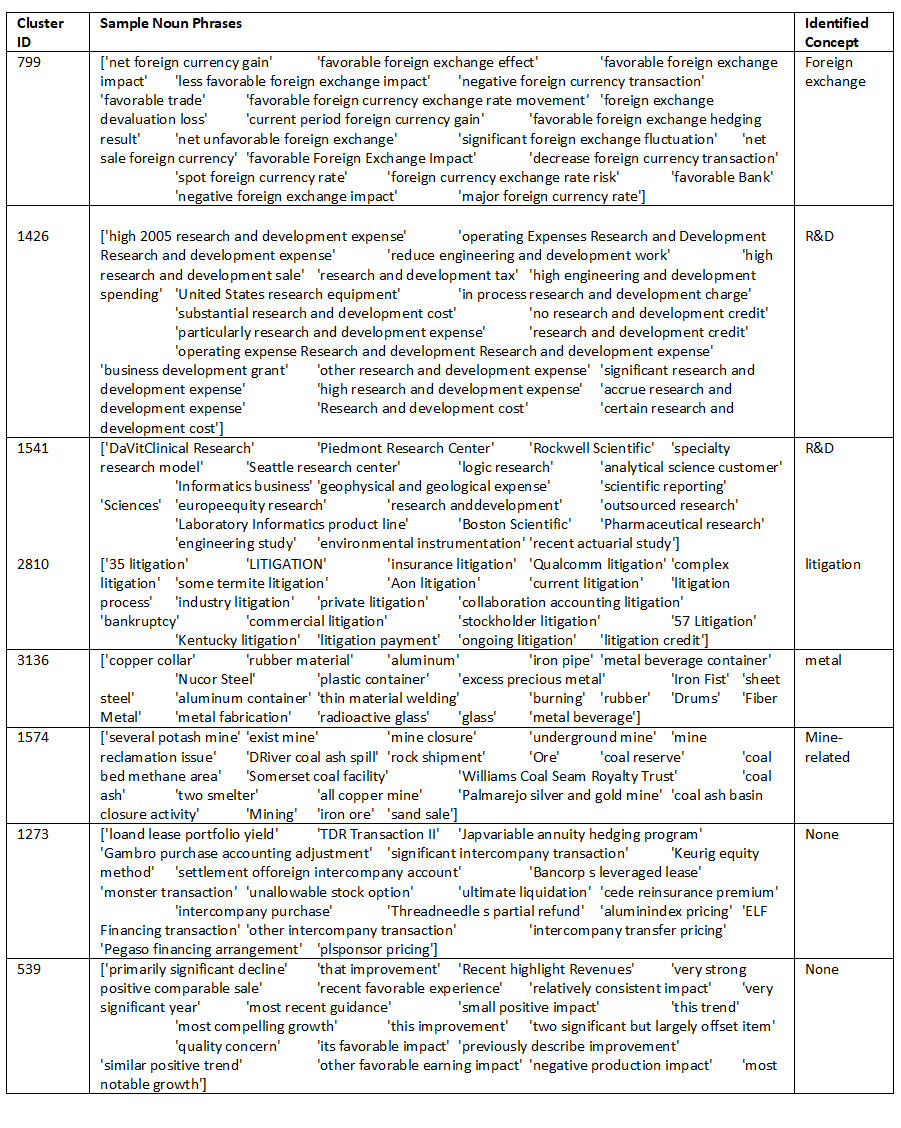
\includegraphics[width=\textwidth]{figures/cluster_samples.png}
  \caption{Examples of the concept clusters sampled from the clustering module output, with the manual identification of 'concepts' from the in-cluster noun phrase samples.}
  \label{fig:cluster_samples}
\end{figure}


This evaluation method is inherently subjective and is limited to the data points sampled from the training set. In the absence of objective ground truths, this evaluation method provides some preliminary indication of the clusters quality. Ultimately, the quality of the clusters is determined by the effectiveness and usefulness of the entire pipeline, which should be judged from the outputs of user queries. Section 4.4 demonstrates a few of such cases.



\section{Use Cases} 

This section demonstrates a few possible applications of the data model in helping to answer the specific investment research questions in Section 3.1. [Add more...]

\subsection{Company's Snapshot and Timeline Evolution}

We can represent the factors affecting a particular company's financial performance by the associated concept clusters distribution on the 2D map based on the SOM grid. When a company's ticker and a time period are specified, we create a query in the data model to collect all the relevant the noun phrases and their respective concept cluster indices, which are then mapped on the SOM grid as a visualization. For example, Figure \ref{fig:netflixlast4} illustrates four snapshots of Netflix in year 2018, 2019, 2020 and 2021, respectively. This way, we can trace the evolution of these factors over time. Moreover, we could also aggregate data at different granularity levels, as illustrated in Figure \ref{fig:netflix5yrs}, where each snapshot corresponds to a successive 5-year period. 

\begin{figure}
     \centering
     \begin{subfigure}[b]{0.45\textwidth}
         \centering
         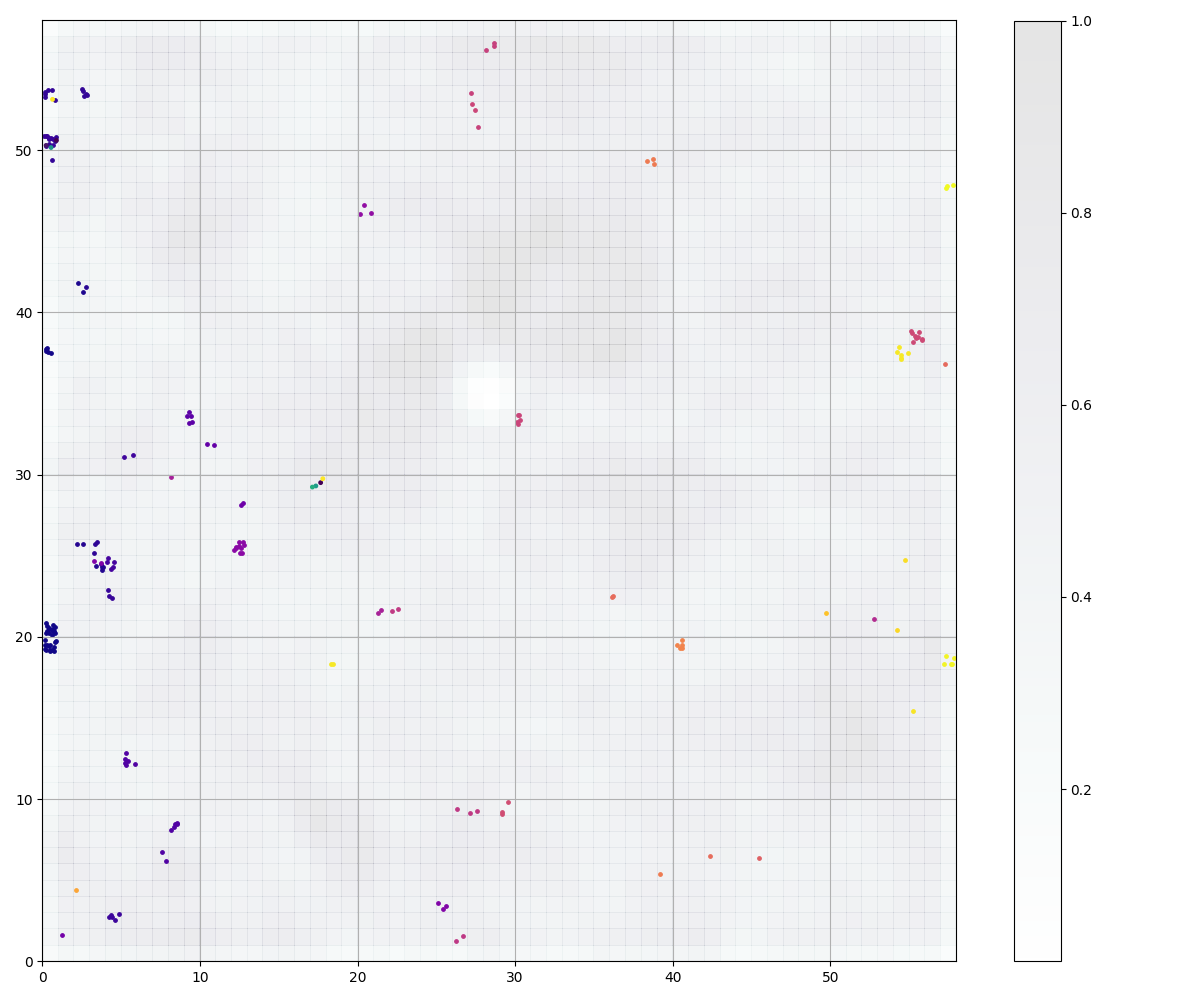
\includegraphics[width=\textwidth]{figures/NFLX_18.png}
         \caption{2018}
     \end{subfigure}
     \hfill
     \begin{subfigure}[b]{0.45\textwidth}
         \centering
         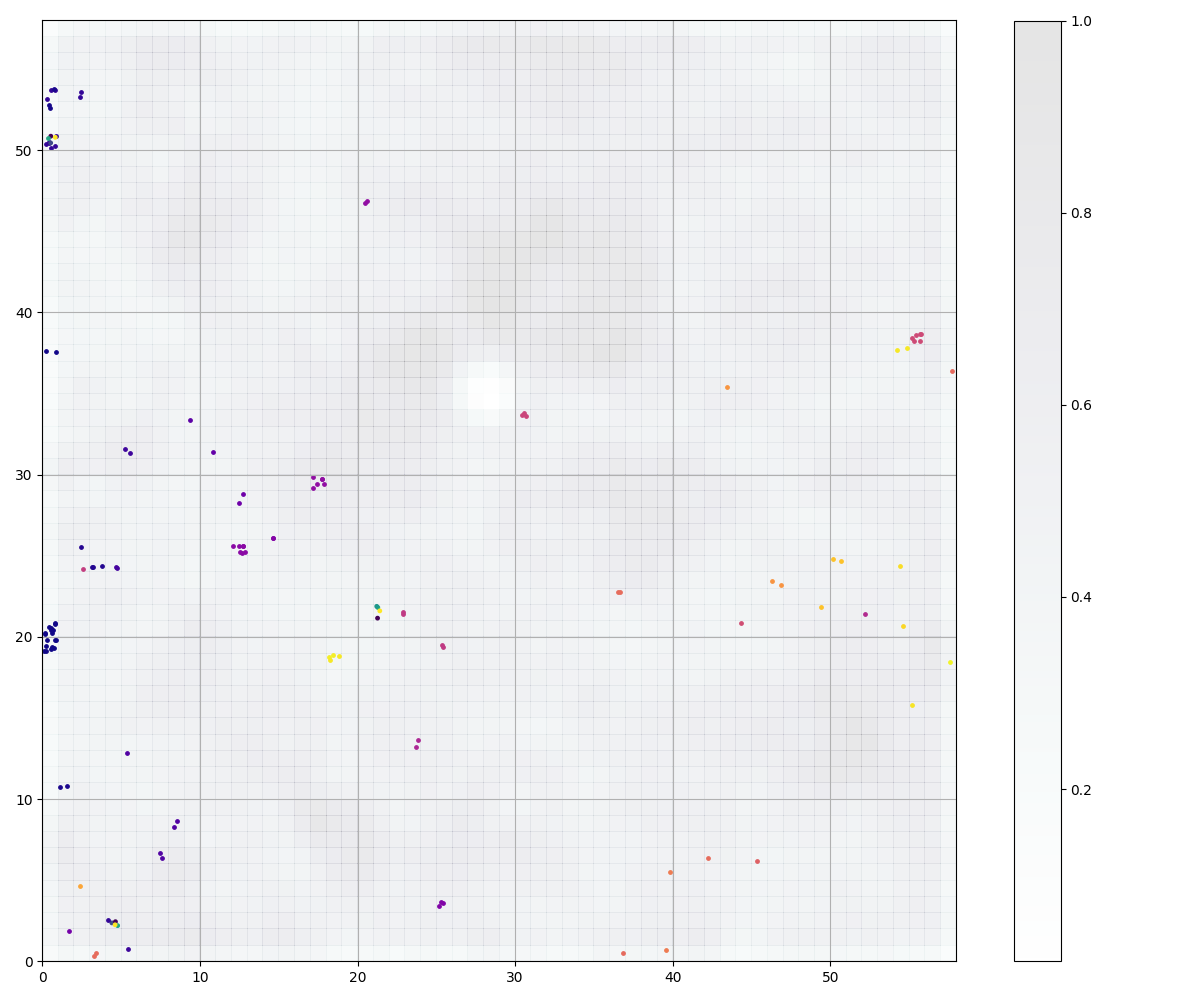
\includegraphics[width=\textwidth]{figures/NFLX_19.png}
         \caption{2019}
     \end{subfigure}
     \hfill
     \begin{subfigure}[b]{0.45\textwidth}
         \centering
         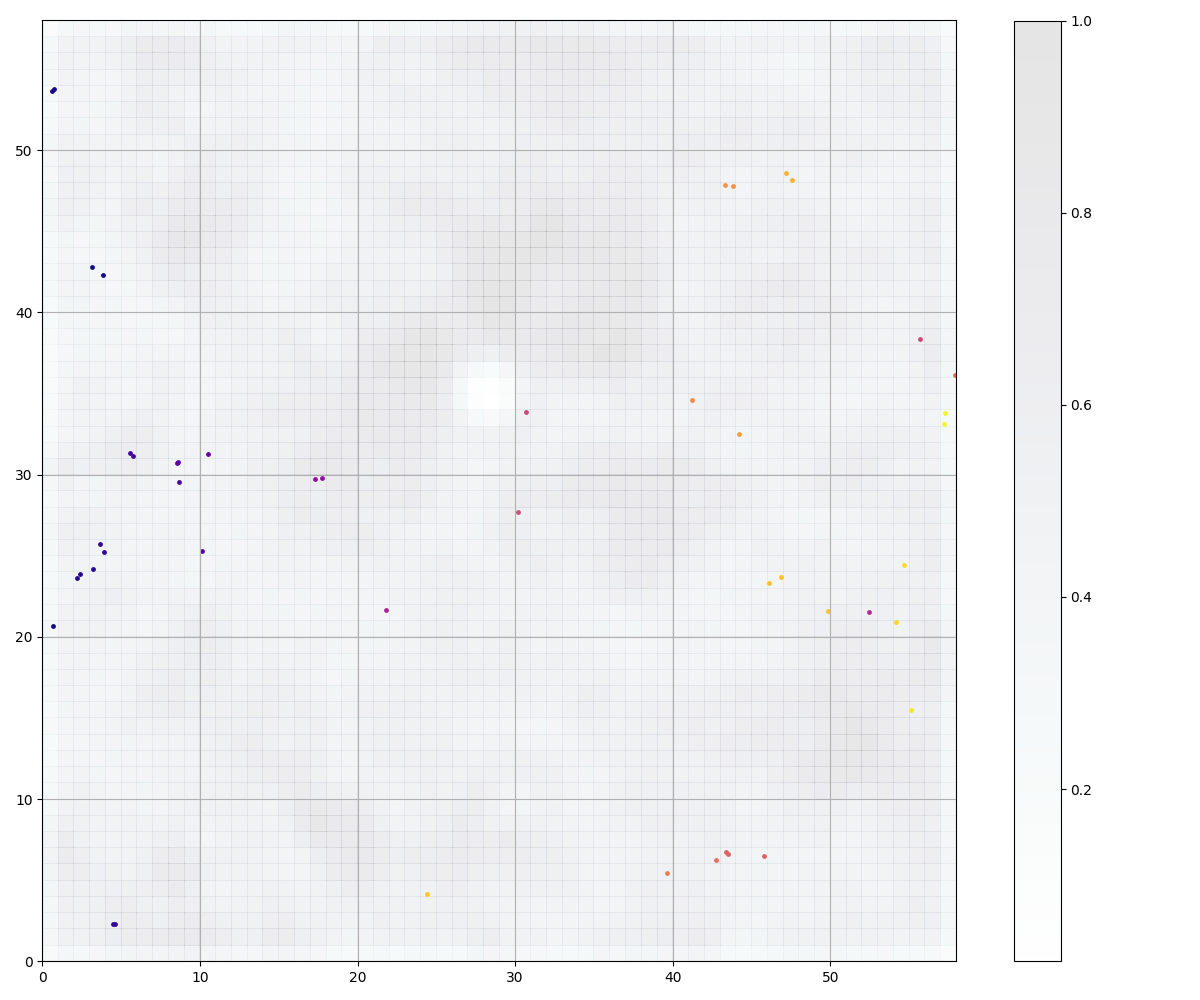
\includegraphics[width=\textwidth]{figures/NFLX_20.png}
         \caption{2020}
     \end{subfigure}
     \hfill
     \begin{subfigure}[b]{0.45\textwidth}
         \centering
         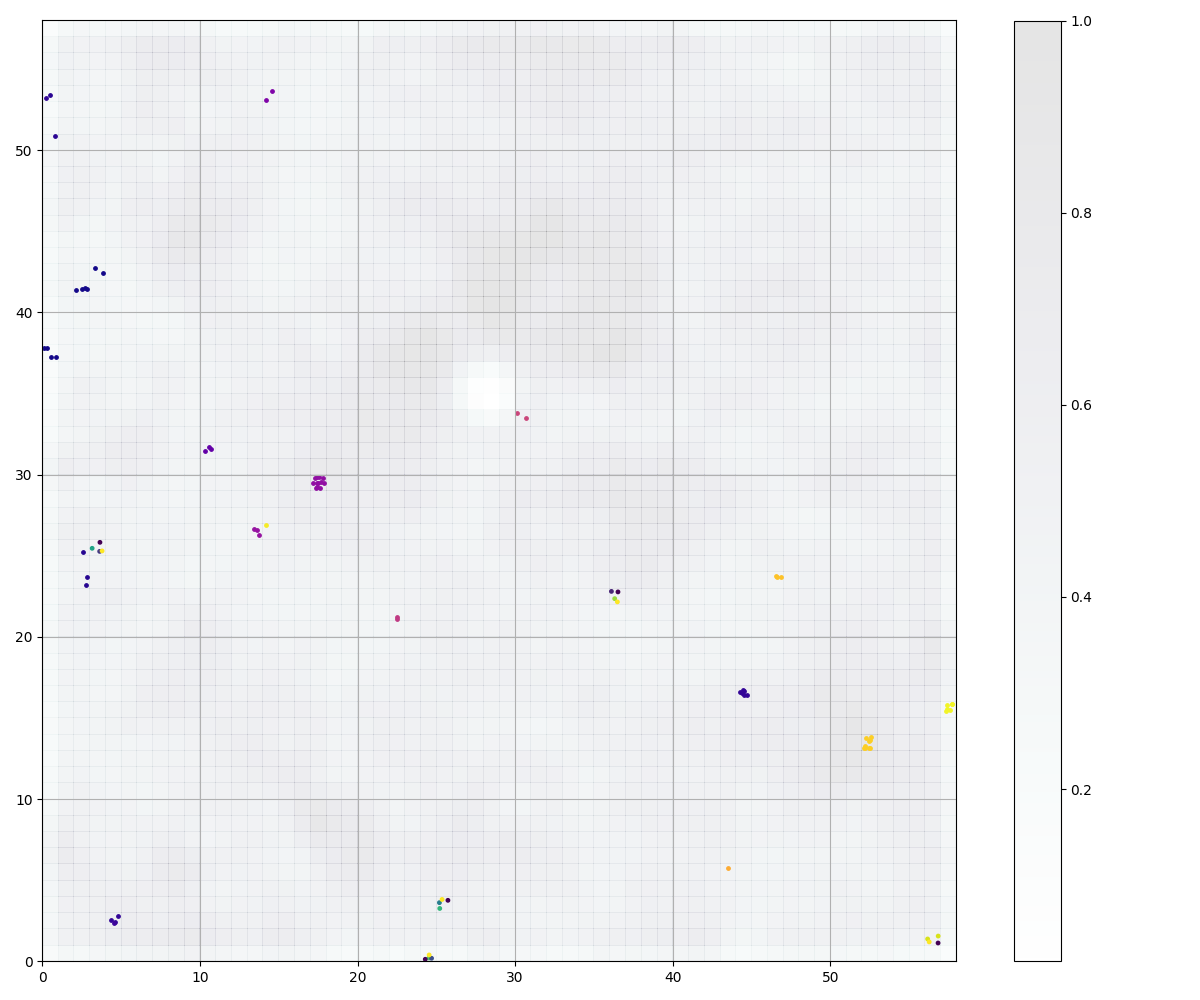
\includegraphics[width=\textwidth]{figures/NFLX_21.png}
         \caption{2021}
     \end{subfigure}
        \caption{Four annual snapshots of Netflix's causal factor map evolution from 2018 to 2021}
        \label{fig:netflixlast4}

\end{figure}




\begin{figure}
     \centering
     \begin{subfigure}[b]{0.45\textwidth}
         \centering
         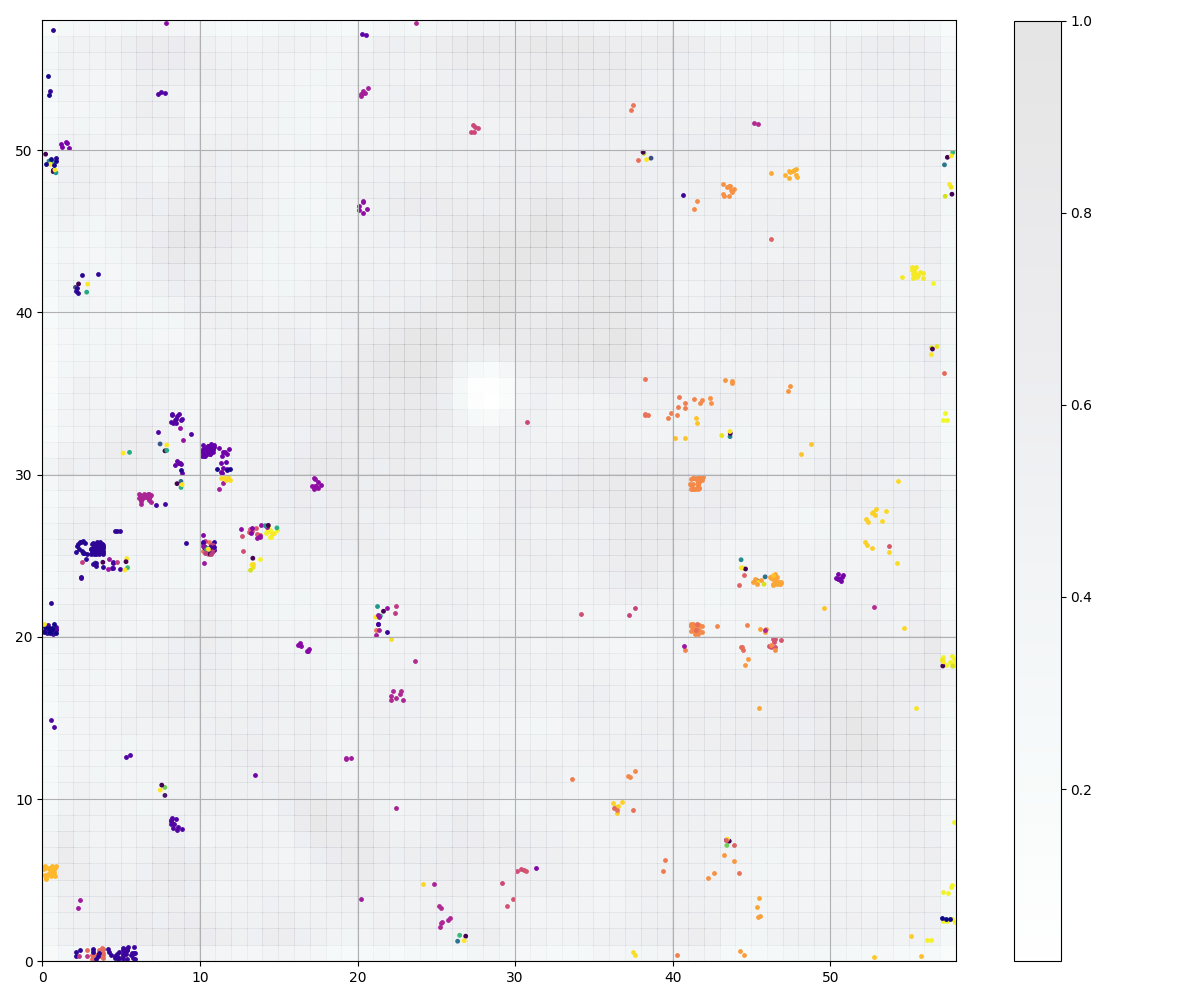
\includegraphics[width=\textwidth]{figures/NFLX_0205.png}
         \caption{2002-2005}
     \end{subfigure}
     \hfill
     \begin{subfigure}[b]{0.45\textwidth}
         \centering
         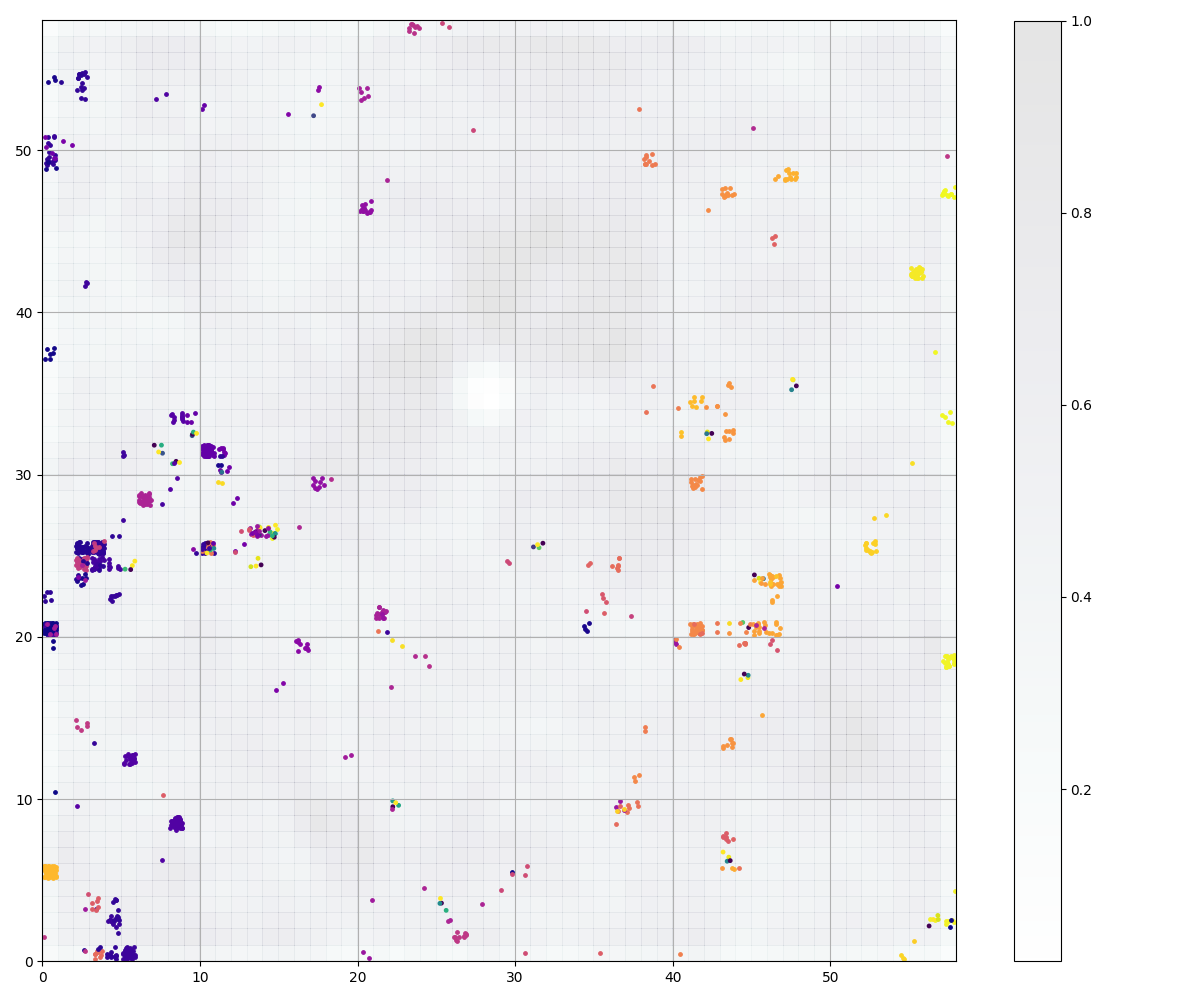
\includegraphics[width=\textwidth]{figures/NFLX_0510.png}
         \caption{2006-2010}
     \end{subfigure}
     \hfill
     \begin{subfigure}[b]{0.45\textwidth}
         \centering
         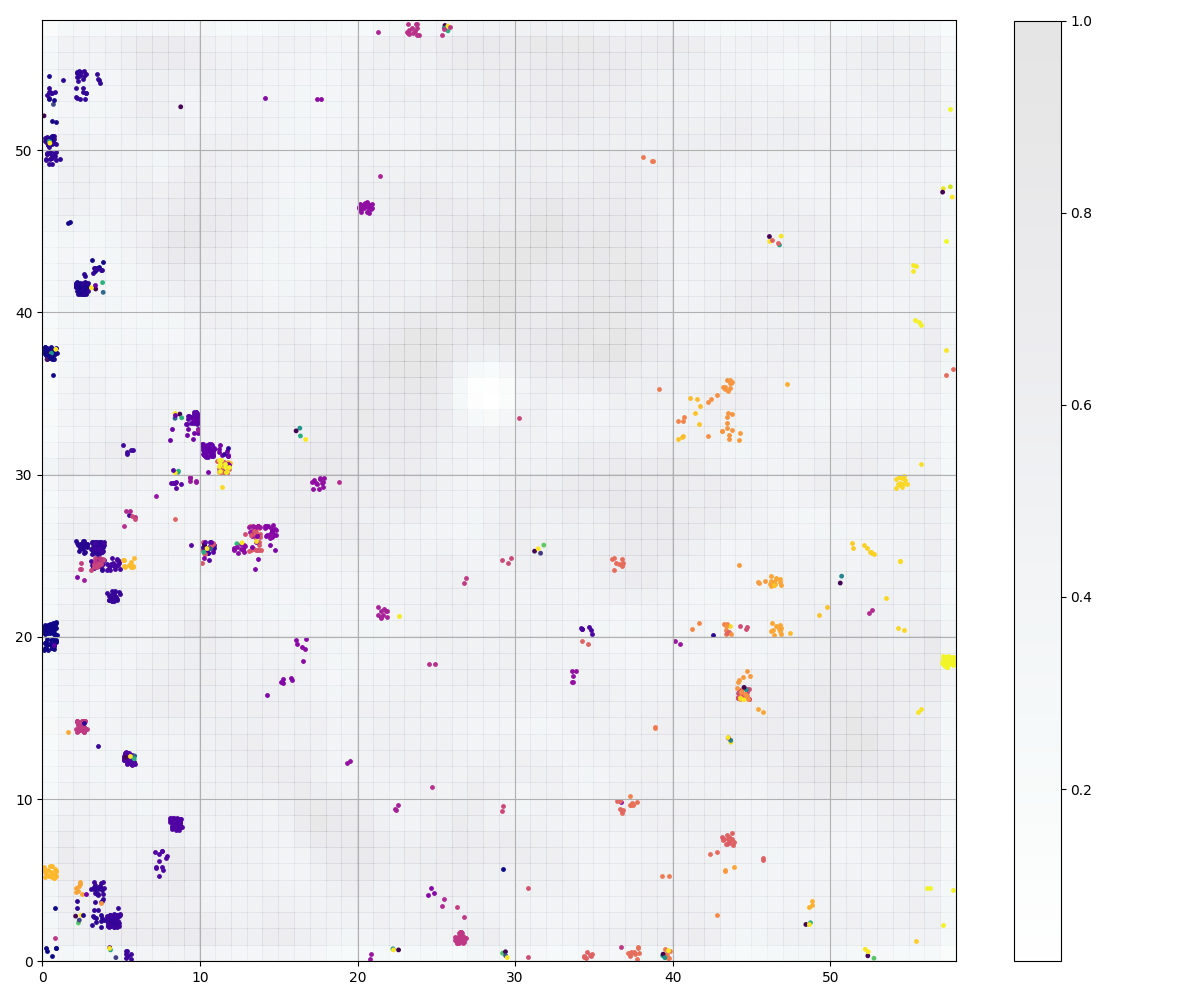
\includegraphics[width=\textwidth]{figures/NFLX_1015.png}
         \caption{2011-2015}
     \end{subfigure}
     \hfill
     \begin{subfigure}[b]{0.45\textwidth}
         \centering
         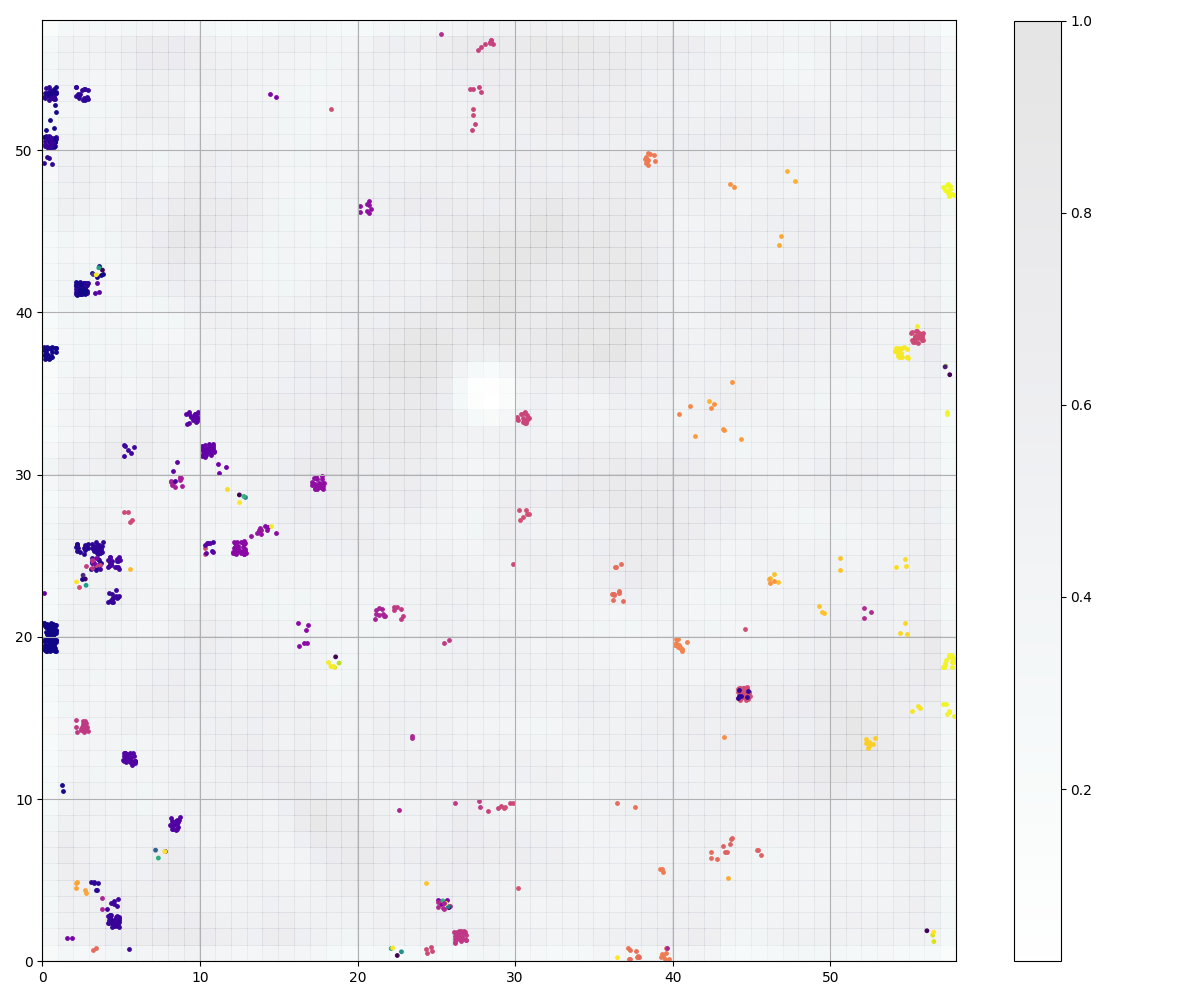
\includegraphics[width=\textwidth]{figures/NFLX_1521.png}
         \caption{2016-2021}
     \end{subfigure}

        \caption{Multi-year aggregated snapshots of Netflix's causal factor map in the last two decades.}
        \label{fig:netflix5yrs}

\end{figure}

By treating these snapshots as a company's signature, we can visually compare maps of two different companies and recognize their distinct patterns. Figure \ref{fig:nflx_ba} shows a side-by-side comparison of Netflix's and Boeing's signature maps aggregated over the last 20 years.  
[add comments on recognizable patterns]

\begin{figure}
     \centering
     \begin{subfigure}[b]{0.45\textwidth}
         \centering
         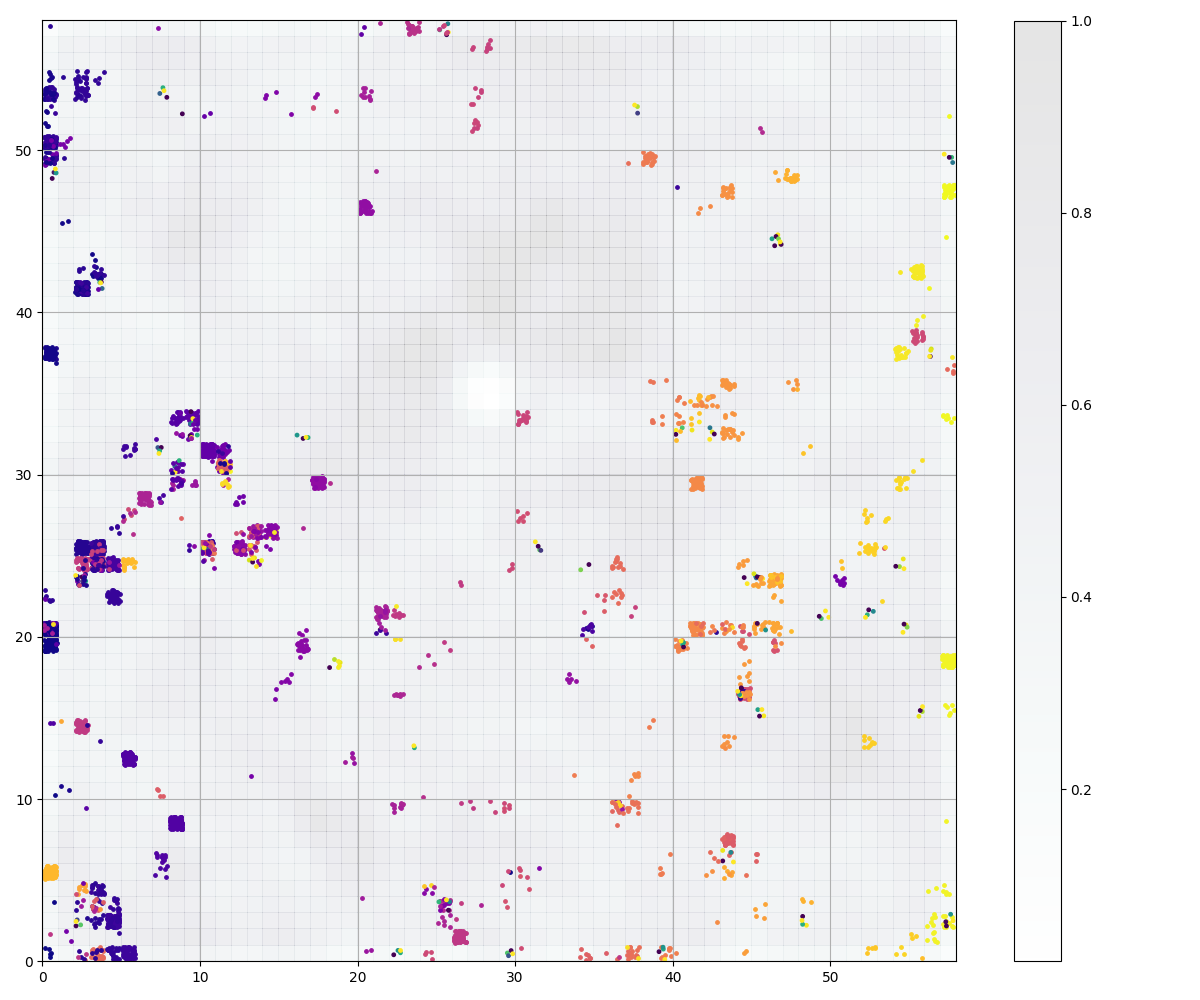
\includegraphics[width=\textwidth]{figures/NFLX_all.png}
         \caption{Netflix}
     \end{subfigure}
     \hfill
     \begin{subfigure}[b]{0.45\textwidth}
         \centering
         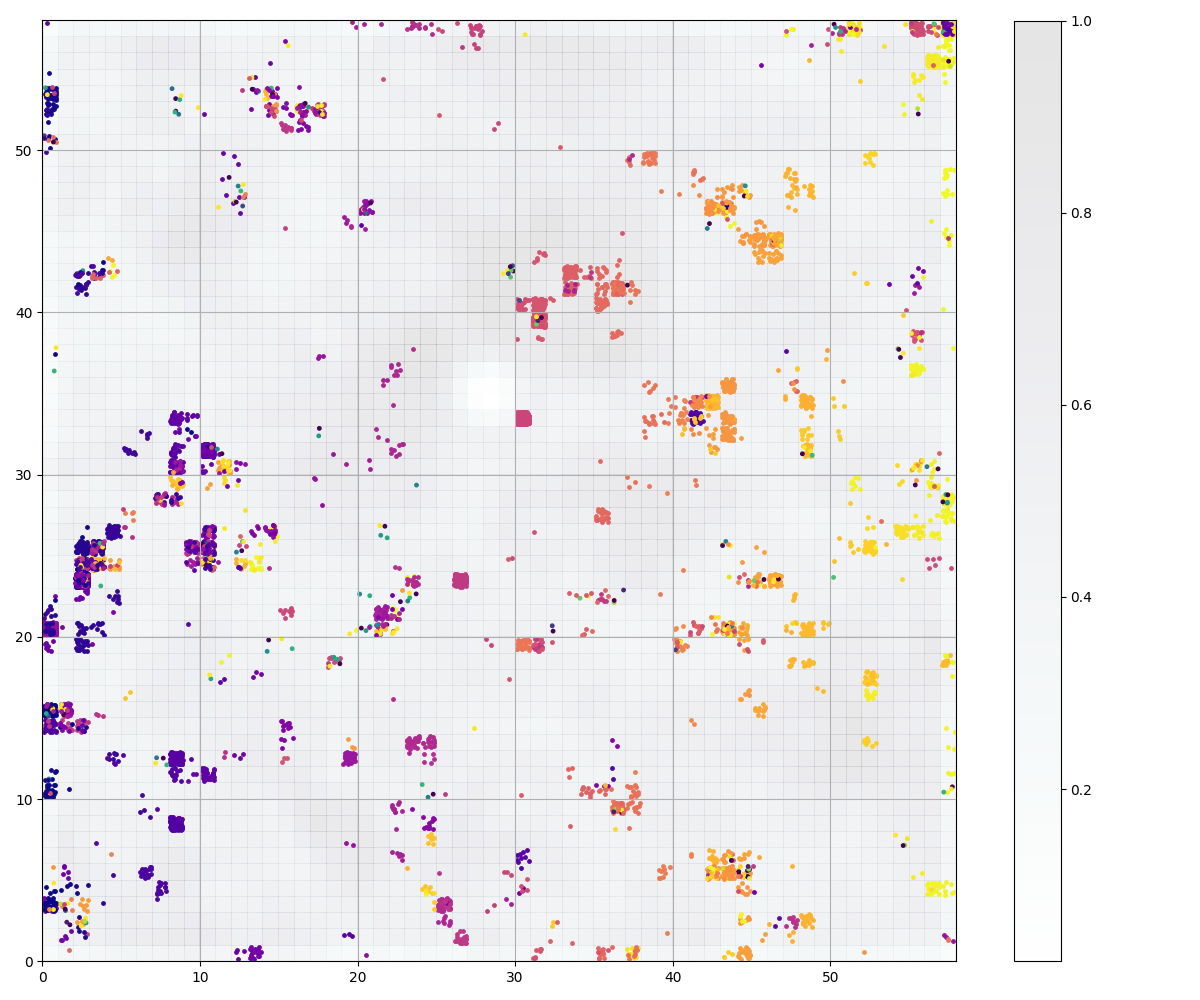
\includegraphics[width=\textwidth]{figures/BA_all.png}
         \caption{Boeing}
     \end{subfigure}

        \caption{Snapshots of Netflix vs. Boeing over the period 2001-2021}
        \label{fig:nflx_ba}
\end{figure}



\subsection{Comparable Companies}

Our data graph also enable users to find the most comparable peers for a target company. Each company can be represented by a vector where each dimension corresponding to a concept cluster. When the time period and topics of interest are specified, the number of links from a particular company to each concept cluster are counted. We calculate the cosine similarity between the target company and a set of potential candidates. These candidate companies can be ranked according to the similarity to the target company. As an illustration, Figure \ref{fig:simMatrix} shows the pairwise cosine similarity matrix of 50 companies. 

For the target company, JP Morgan Chase, for example, the top 5 most similar companies are:
\begin{itemize}
	\item 1. Wells Fargo \& Company (cosine similarity = 0.611)
	\item 2. At\&T (cosine similarity = 0.577)
	\item 3. Citigroup (cosine similarity = 0.531)
	\item 4. Chubb Ltd (cosine similarity = 0.501)
	\item 5. Marsh \& McLennan Companies (cosine similarity = 0.500)
\end{itemize}

[TO DO: discuss how it can be further improved by merging similar concept clusters together]

\begin{figure}
     \centering
     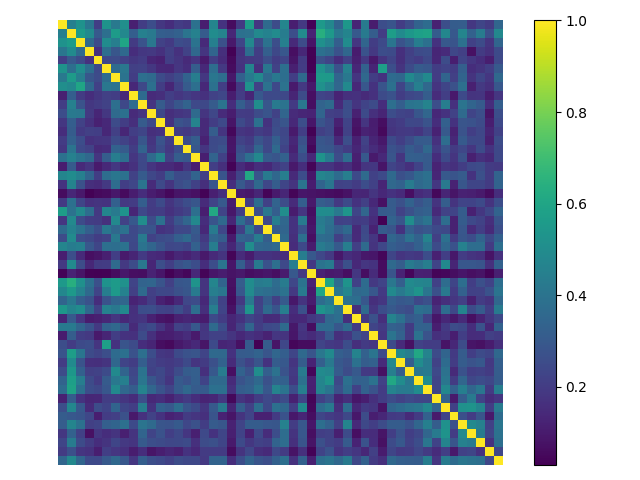
\includegraphics[width=0.7\textwidth]{figures/SimilarityMatrix.png}
     \caption{Cosine Similarity Matrix of 50 Companies}
	\label{fig:simMatrix}
\end{figure}




\subsection{Keyword Search for the Most Relevant Companies}
Another use case that can be envisaged is for the user to input a few key words and search for the most relevant companies. For instance, a user might be interested to find out which companies are most likely to be affected by price fluctuations in agriculture commodities with the specified input keywords: \emph{"wheat", "corn", "soybean"} and \emph{"meat"}. 

Our system first converts these keywords into word embeddings, which are fed into the clustering module one by one to find the most relevant set of concept clusters associated with these keywords. In the sample above, the set of concept clusters identified by our system are demonstrated in Table \ref{table:kwsearch}. Next, we define a query in Cypher to traverse the graph data model and collect all the companies that are connected to these identified concept clusters. We rank the companies by aggregating the total number of links to the set of concept clusters. 

\begin{table} 
\small
\centering
\begin{tabular} {| m{5em} | m{4em} |m{26em} |}
\hline
Keyword & \ Concept Cluster Index & \ Sample Noun Phrases from the Cluster\\ 
\hline
wheat & 2435 & \emph{rise dairy, acreage sale, Crop Protection, improved corn processing, seasonal purchasing, seasonal hog supply, weak harvest, cattle supply, lower plant acreage}\\ 
\hline
corn &2377 & \emph{new acreage, large harvest, concentrated phosphate crop, seasonal crop, grower activity, primarily cotton, less bountiful harvest, low hog harvest, Harvest} \\
\hline
soybean & 2435 & \emph{poor crop, potential sorghum duty deposit, oat supply, reduce crop production, increase cereal acre, reduce corn sale, wheat product, rise cattle, pork supply shortage}\\ 
\hline
meat & 2203 &\emph{pizza, Habit Burger Grill, deli item, taco, Premium Chicken Sandwiches, frozen pizza, meat ingredient, Chicken, Chipotle restaurant} \\ 
\hline
\end{tabular}
\caption{Concept Clusters identified by the clustering}
\label{table:kwsearch}
\end{table}


In the above example, our system outputs the following companies as the most relevant to the input search terms:

\begin{itemize}
	\item 1. General Mills: manufacturer and marketer of branded consumer foods (234 links)
	\item 2. Tyson Foods: meat processor and marketer (203 links)
	\item 3. Campbell Soup: processed food and snack company (151 links)
	\item 4. Zoetis: a global animal health company (109 links)
	\item 5. Archer-Daniels-Midland: food processing and commodities trading corporation (104 links)
\end{itemize}


Table \ref{table:searchexamples} shows a few other examples in keyword search. Note that the output of this search is only meant for providing a rough indication ... [add comments]

\begin{table} 
\small
\centering
\begin{tabular} {| m{15em} |m{25em} |}
\hline
Keywords & \ Top 5 Most Relevant Companies \\ 
\hline

aircrafts, flights, fuel price & Alaska Air Group, Southern, American Airlines Group,  
United Parcel Service, Southwest Airlines \\
\hline
cloud computing, business analytics, cloud storage, data management &
Amazon, Akamai Technologies, CF Industries Holdings, Northrop Grumman, Equinix \\
\hline
global supply chain disruption, inflation, pandemic, Covid-19 & Prudential Financial, Metlife, Sysco, United Parcel Service, Cognizant Technology Solutions\\
\hline
\end{tabular}
\caption{Further examples in keyword search}
\label{table:searchexamples}
\end{table}







\newpage

%%%%%%%%%%%%%%%%%%%%%%%%%%%%%%%%%%%%%%%%%%%%%%%%%%%%%%%%%%%%

\chapter {Conclusion} \label{conclusion}


% \chapter {Conclusion} \label{conclusion}

\section{Discussion}  

%(1 page) The most important results and findings of the work are summarised (not simply a repetition of the structure of the previous chapters!), which new concepts, methods and tools have been developed, which problems can now be solved (more efficiently),

% key contributions
In this thesis, we have presented a text mining tool to extract causality from financial documents. We have also designed a heterogeneous graph-based data model to store the extracted information and to faciliate data exploration. Furthermore, we have demonstrated how this model can be used to assists financial analysts to solve specific, practical problems in investment research.

% causality extraction and practical considerations
After a comprehensive survey of causality extraction techniques, we have decided to adopt a linguistic pattern-based approach, rather than using the latest deep learning models with supervised training. This design choice is based on practical limitations such as avaialblity of training data, cost of annotation, model intepretability, etc. Also taking into consideration is the structure of financial reports and the language styles [TODO] making the linguistic approach possible. Indeed, the causality extraction module has achieved a satisfactory performance level with an overall F1-score of 90\%, albeit the benchmarking dataset is relatively small. This shows that for domain-specific problems, the simpler method might work as well as the most advanced sophisciated methods but with the added practical advantage of saving cost and time.


% clustering
To mimic In order to translate the ... into ... 

To facilitate 


% data exploration and visualization


By systematically extracting causal factors from financial text, and storing them in a graph database, time and cost reduction can be achieved. 

\section{Future Work} 
% (1 page) an outlook on what is to come (e.g. ~What would you do if you had 6 months more time).


\newpage

%%%%%%%%%%%%%%%%%%%%%%%%%%%%%%%%%%%%%%%%%%%%%%%%%%%%%%%%%%%%

\appendix 

\chapter{Appendix}

\section{Papers on Causality Extraction}
\label{appendix:CEpapers}

\begin{figure}[h!]
\centering
  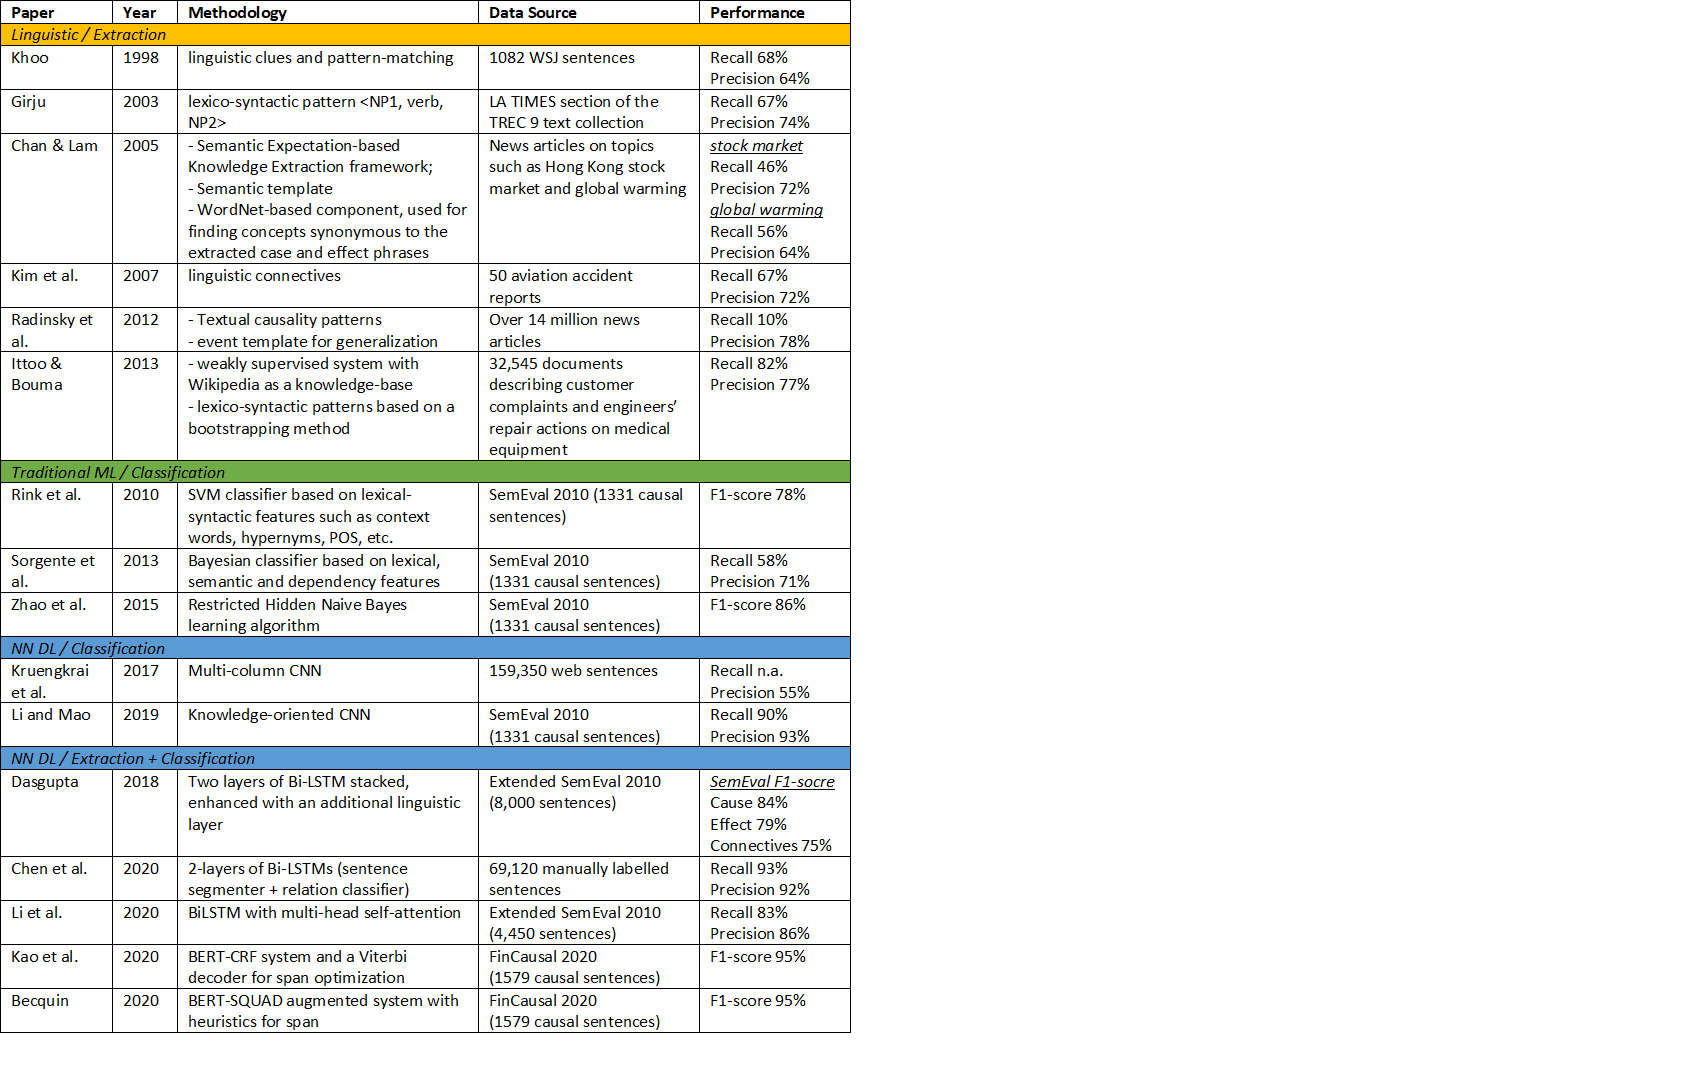
\includegraphics[scale=0.9]{figures/CE_papers.png}
  \caption{a summary table of all the papers relevant to causality extraction reviewed for this thesis.}
\end{figure}


\section{Exploratory Data Analysis on Raw MD\&A Texts} \label{appendix:EDA}

\begin{figure}
    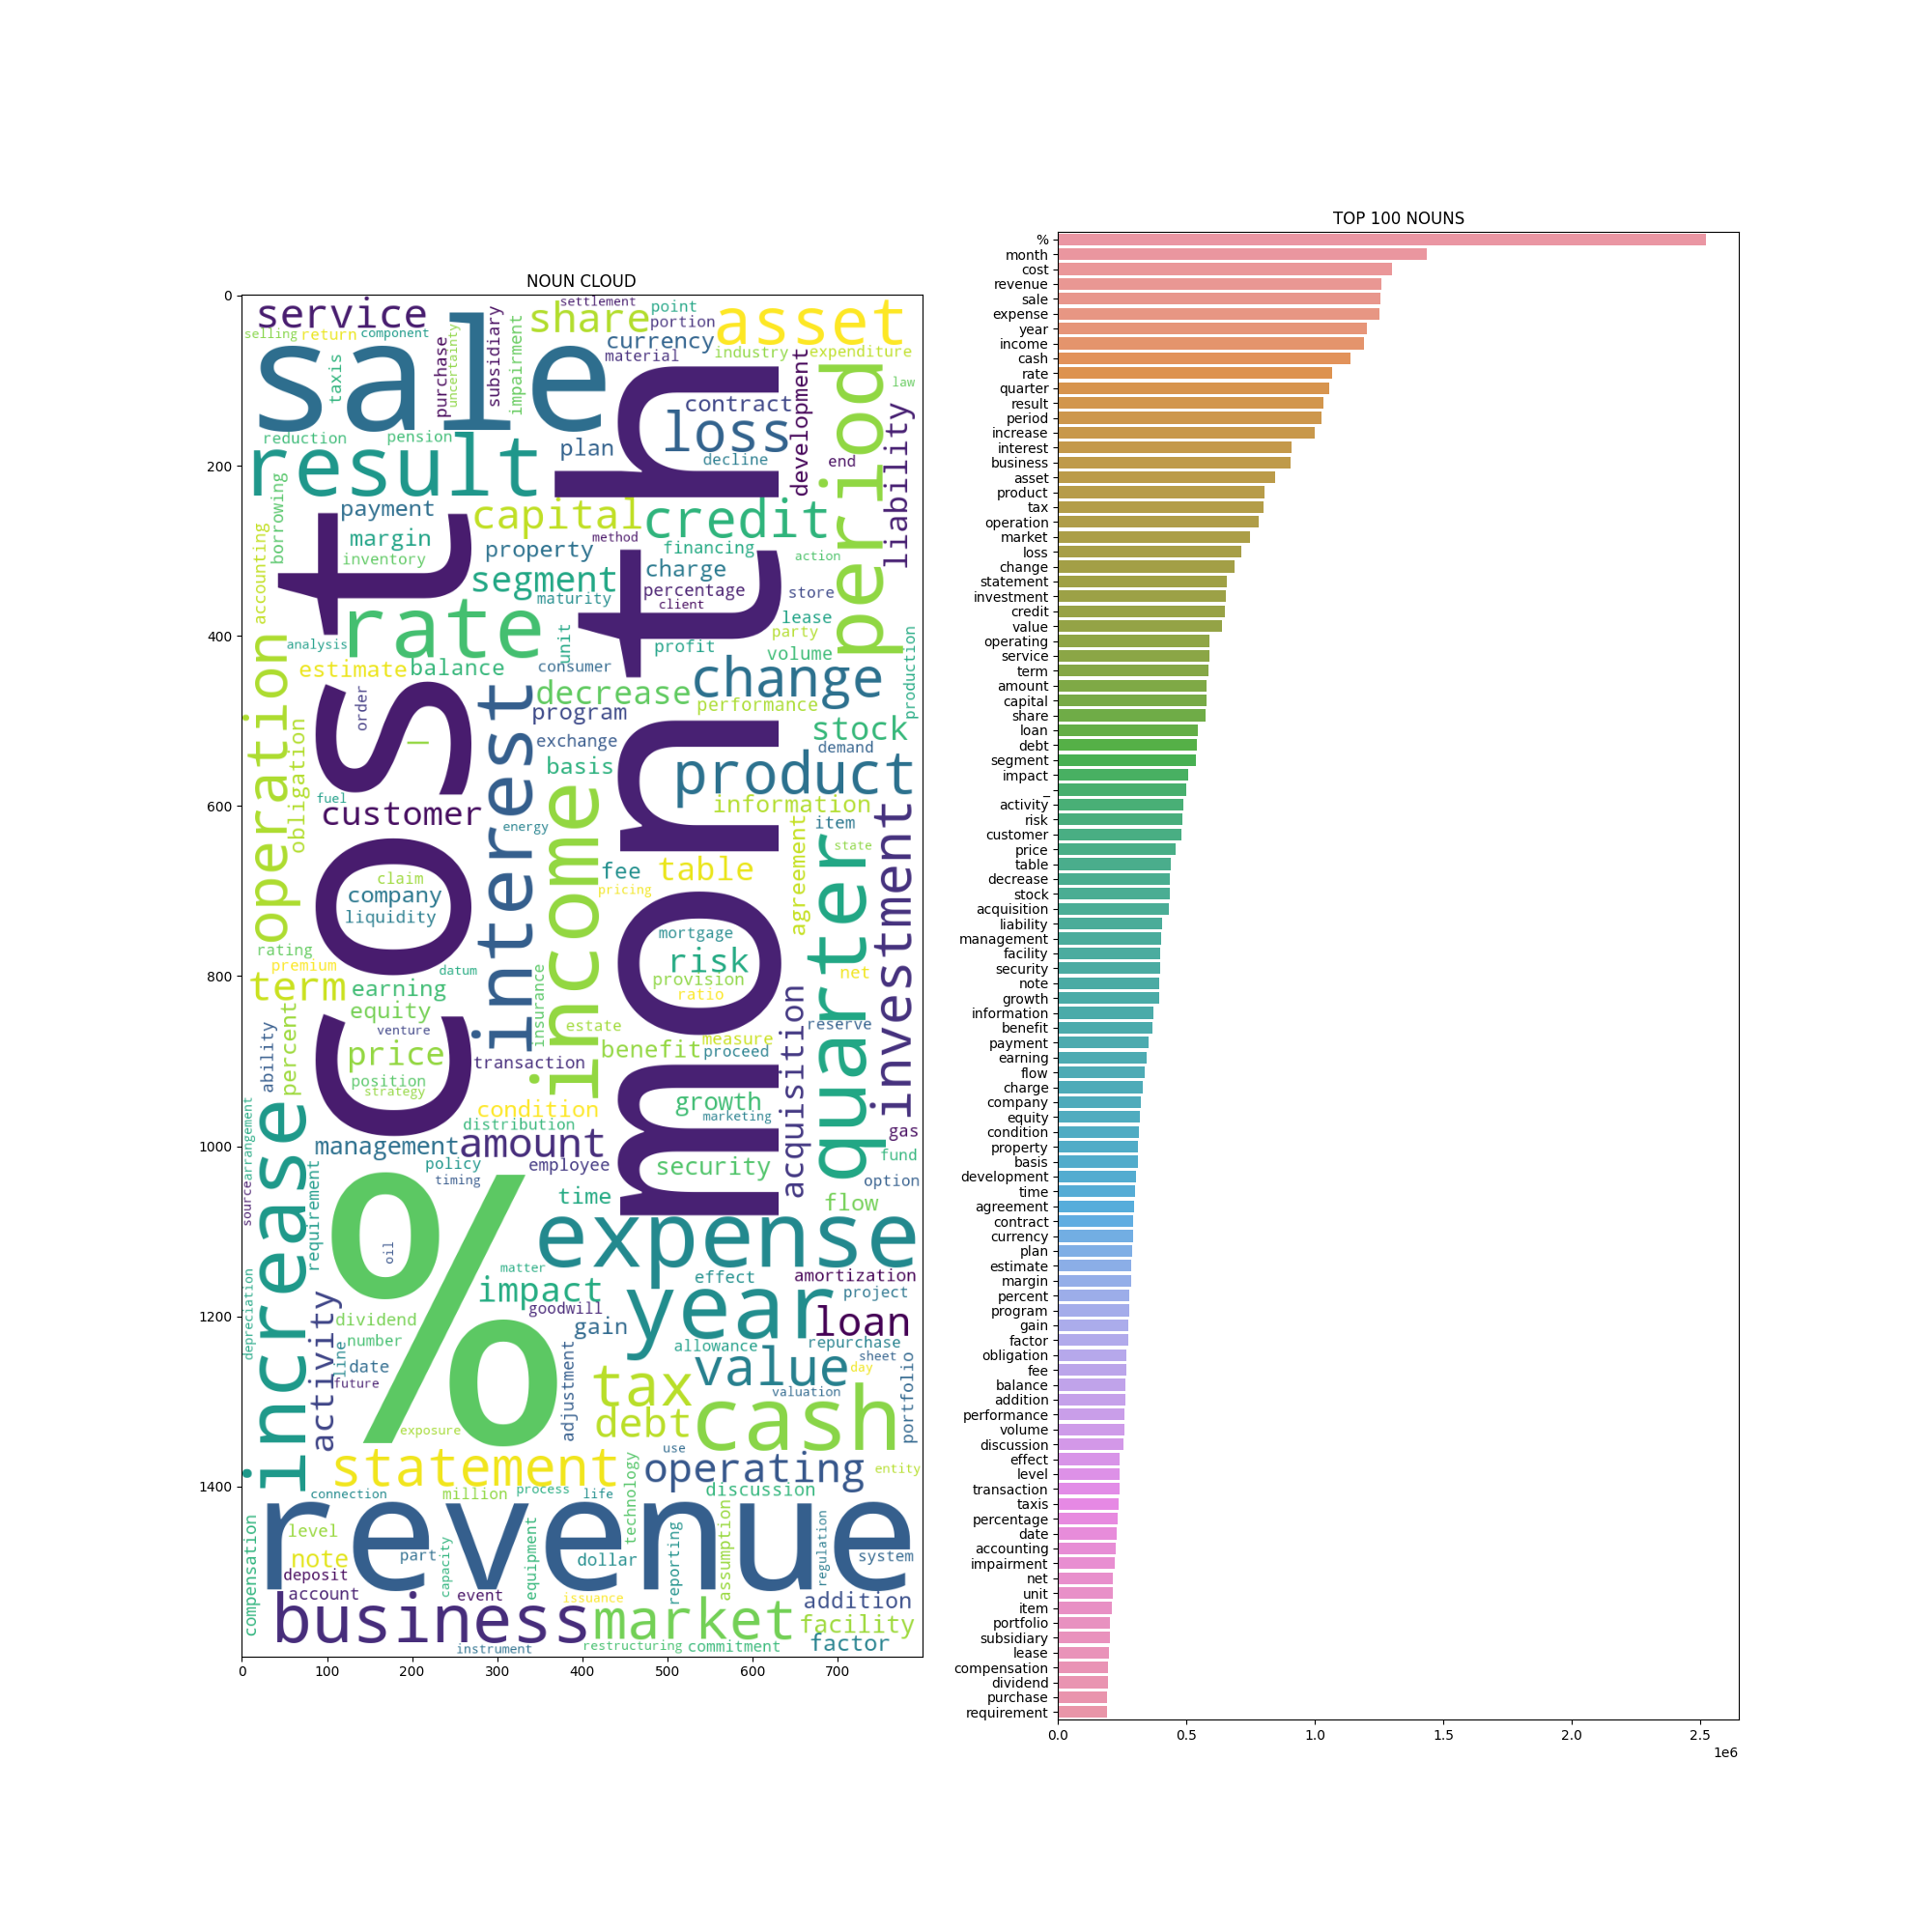
\includegraphics[width=\textwidth] {figures/NOUN_top100_figure.png}
    \caption{Word Cloud of Top 100 Nouns}
    \label{fig:NOUN}
\end{figure}

\begin{figure}[!tbp]
    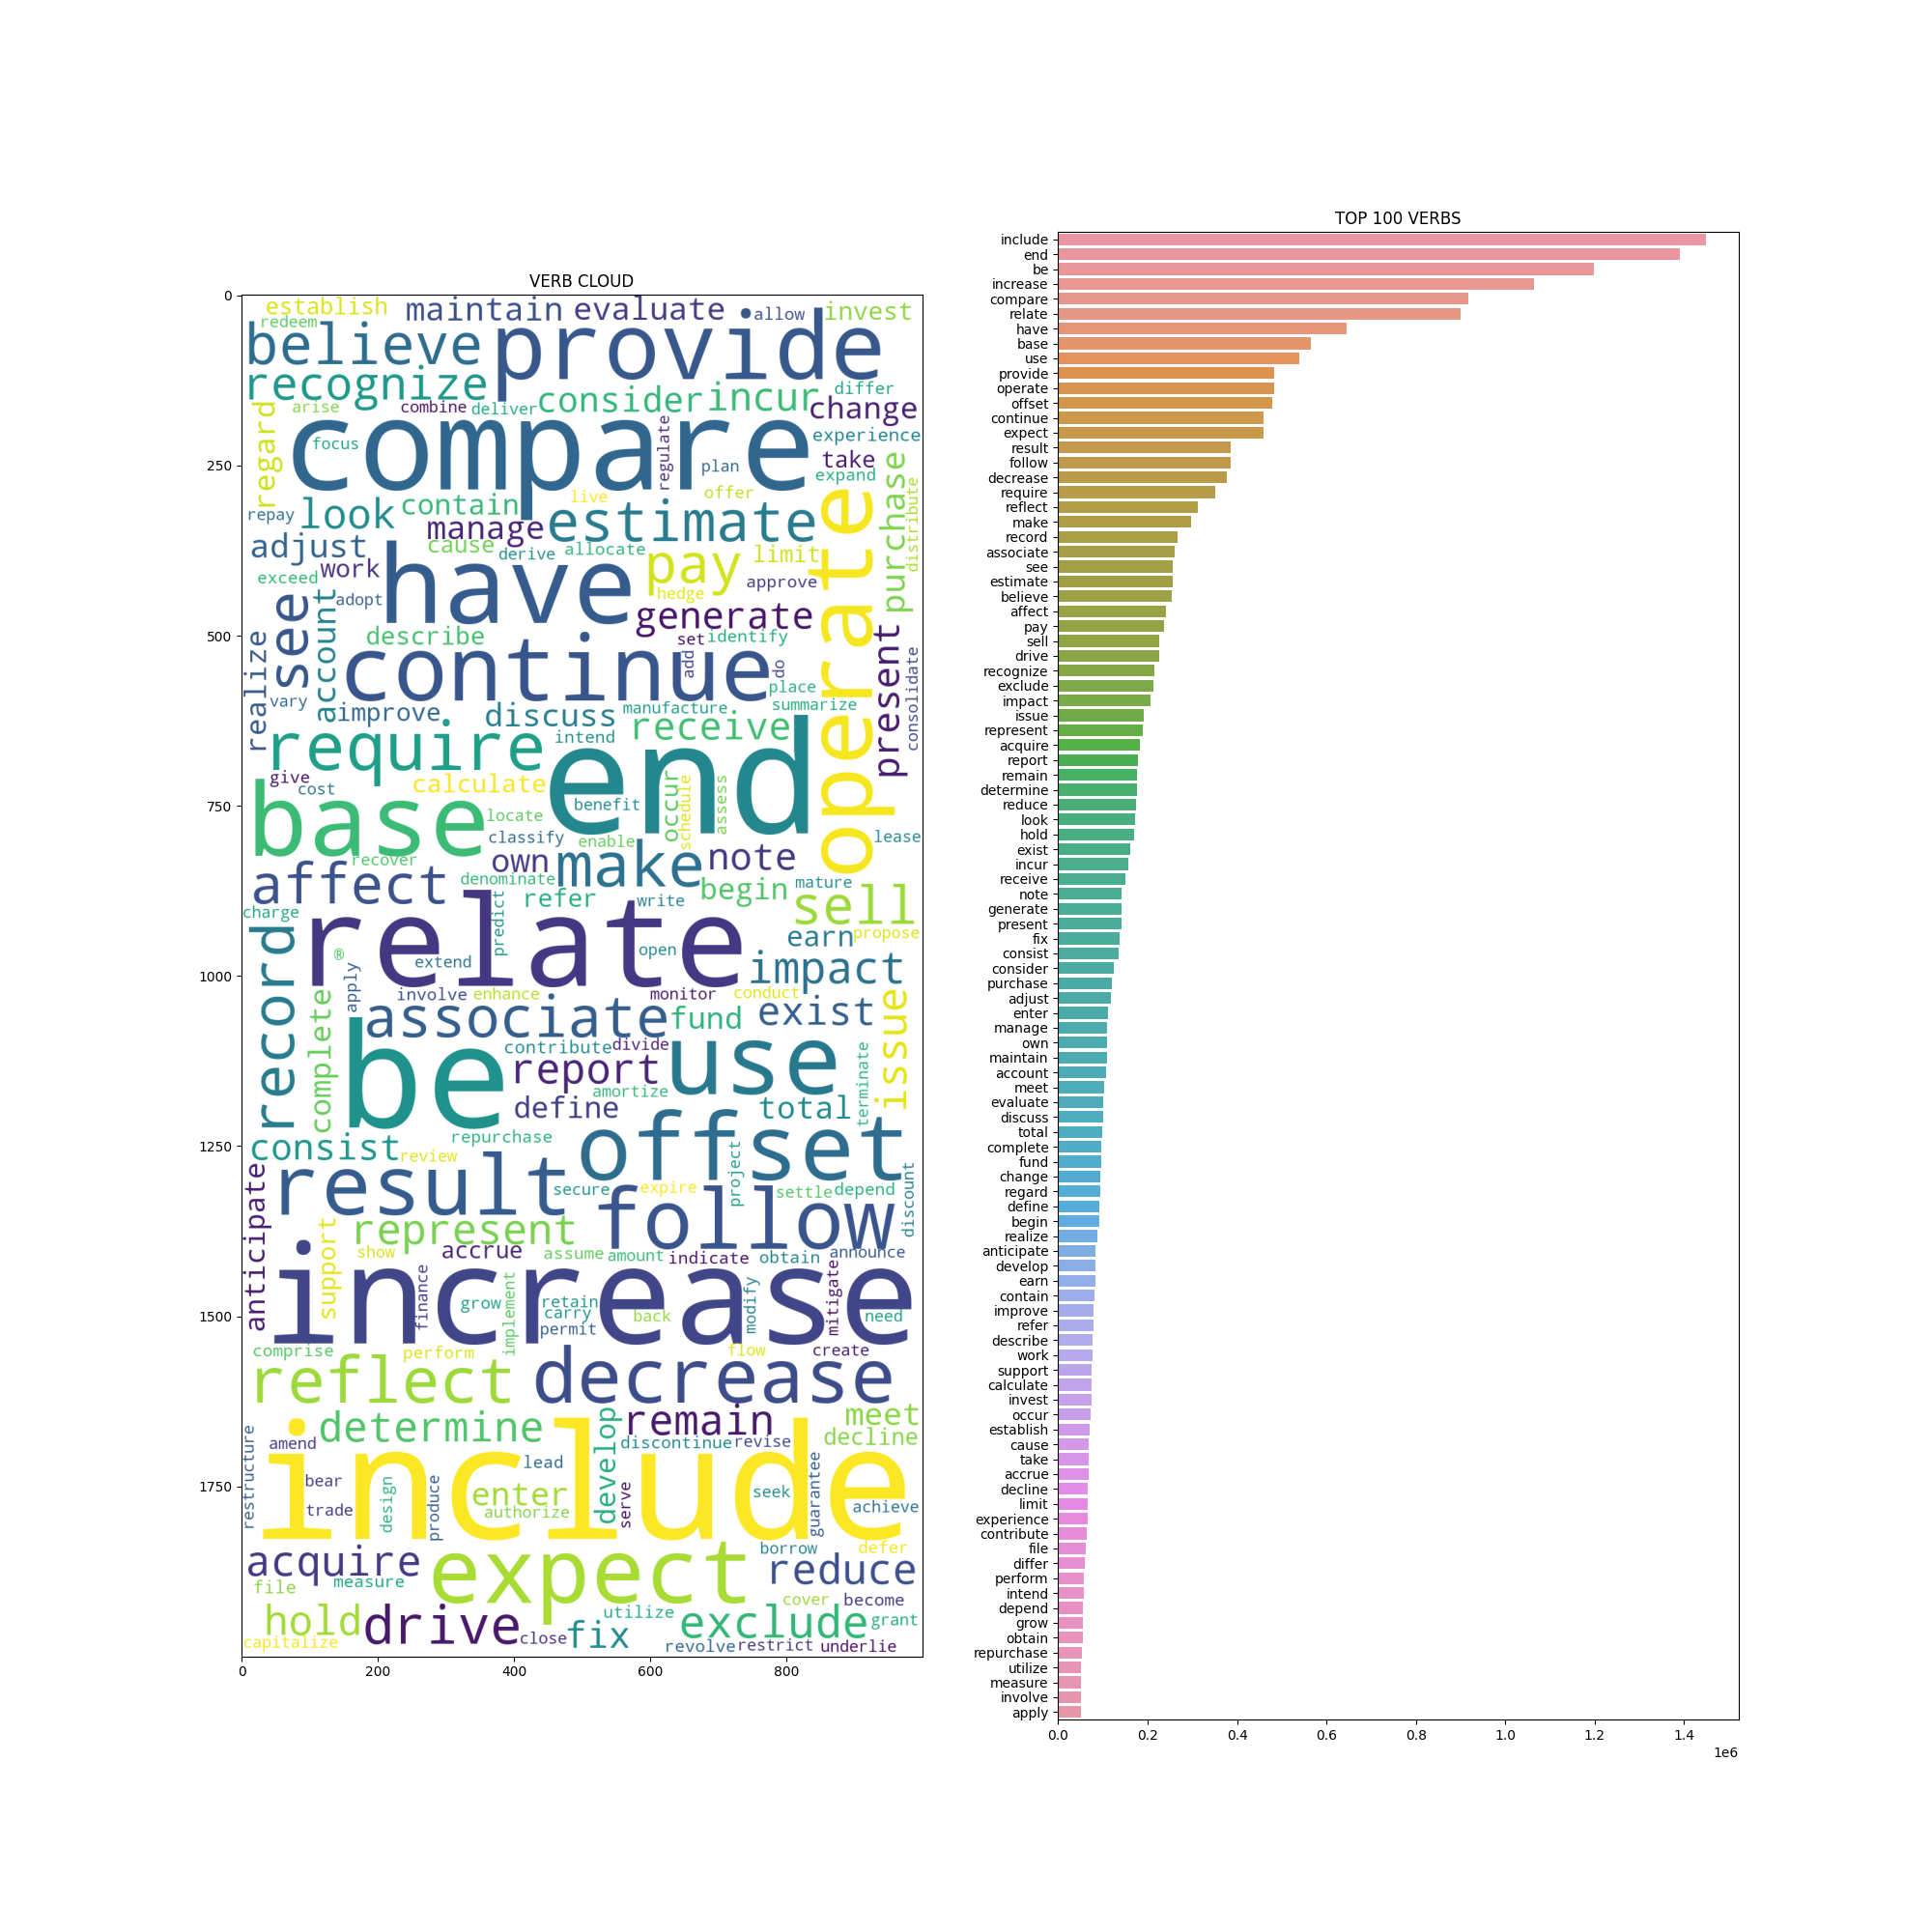
\includegraphics[width=\textwidth]{figures/VERB_top100_figure.png}
    \caption{Woud Cloud of Top 100 Verbs}
    \label{fig:VERB}
\end{figure}



\newpage

% References (Literaturverzeichnis):
% a) Style (with abbreviations: use alpha):
% see https://de.wikibooks.org/wiki/LaTeX-W%C3%B6rterbuch:_bibliographystyle
% for the different formats and styles
\bibliographystyle{ieeetr} %{apalike}

% b) The File:
\bibliography{references}

\end{document}
